\chapter{Survey of existing practice}\label{sec:survey-existing-practice}

%\protect\hypertarget{h.2hcxkn16a7yd}{}{}

Statewide modeling is becoming
mainstream in the U.S. In 2005, 20 of the 50 U.S. states had implemented operational statewide models \citep{horowitz06}. The survey conducted in 2016 for this synthesis report revealed that 34 states (out of 46 states that responded in 2016) operate statewide models, an increase of 70 percent over 11 years.

\section{Survey findings}

The survey of state agencies was a key source of information about the state of practice in statewide modeling in the U.S. However, as with any survey, the results reflect how the respondents understood the question, which in some cases may not have perfectly matched its intent. There are likely to be some important nuances and elements of context in all the responses that are impossible to fully capture in a standardized survey. While the discussion in this section represents the state of practice in the U.S. at large, individual responses may have been imprecise due to misunderstanding or limited familiarity with the topic of a question. The difficulties found when summarizing results will be discussed in more detail in \S\ref{sec:survey-critical-review}. Nevertheless, the overall state of practice in statewide modeling is presumed to be represented accurately in this section.

The survey conducted for this synthesis report was divided into eight parts. One of these parts, Scenarios, was already discussed in \S\ref{sec:scenario-analysis} (page \pageref{sec:scenario-analysis}). The following detailed description of survey results follows the structure of the remaining seven principal parts, namely person travel demand model, person long-distance model, freight model, economic model, land use model, environmental impact model, and resources. The chapter will end with some summarizing remarks on survey findings.

\section{Person travel demand modeling}\label{sec:person-demand-modeling}

The survey started with a question about the type of person travel demand model implemented or under development. For the states that distinguish between short and long-distance travel this initial part of the survey referred to short-distance travel only. Many states, however, do not operate a separate long-distance model. For those states, the following answers refer to both short and long-distance travel. The traditional four-step modeling paradigm is applied in 26 states, as shown in Figure \ref{fig:person-model-frequency}. This includes some states that model auto travel only and skip the mode choice step (making it essentially a three-step model with trip generation, trip distribution, and assignment). This category also includes states that split traffic into various periods of time, making it a five-step model. It should be noted, however, that many states apply this four-step concept to short-distance travel only, using a different modeling approach for long-distance travel. Five states are in the process of developing a four-step transportation model. Four other states have an operational activity-based model, with two more states developing such models.

\begin{figure}
\centering
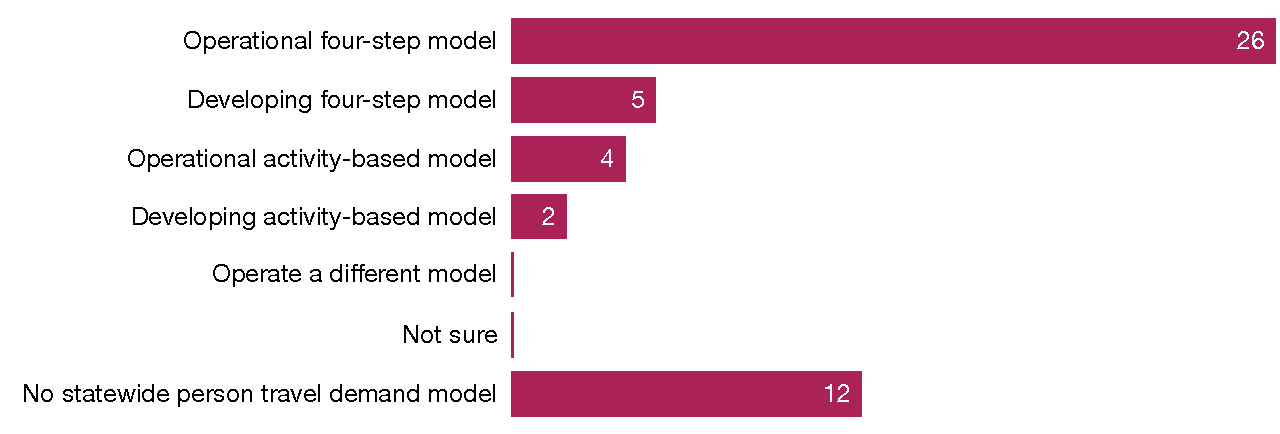
\includegraphics[scale=0.65]{graphics/05-person-demand-model-types}
\caption[Frequency of travel demand model types for person travel]{Frequency of travel demand model types for person travel (multiple answers allowed)}
\label{fig:person-model-frequency}
\end{figure}

The spatial distribution of different model types across the nation is shown in Figure \ref{fig:statewide-modeling-status}. Activity-based models are more common in the Western part of the U.S., with Ohio and soon Maryland being the only two states in the eastern part of the country using them.

\begin{figure}   % 6
\centering
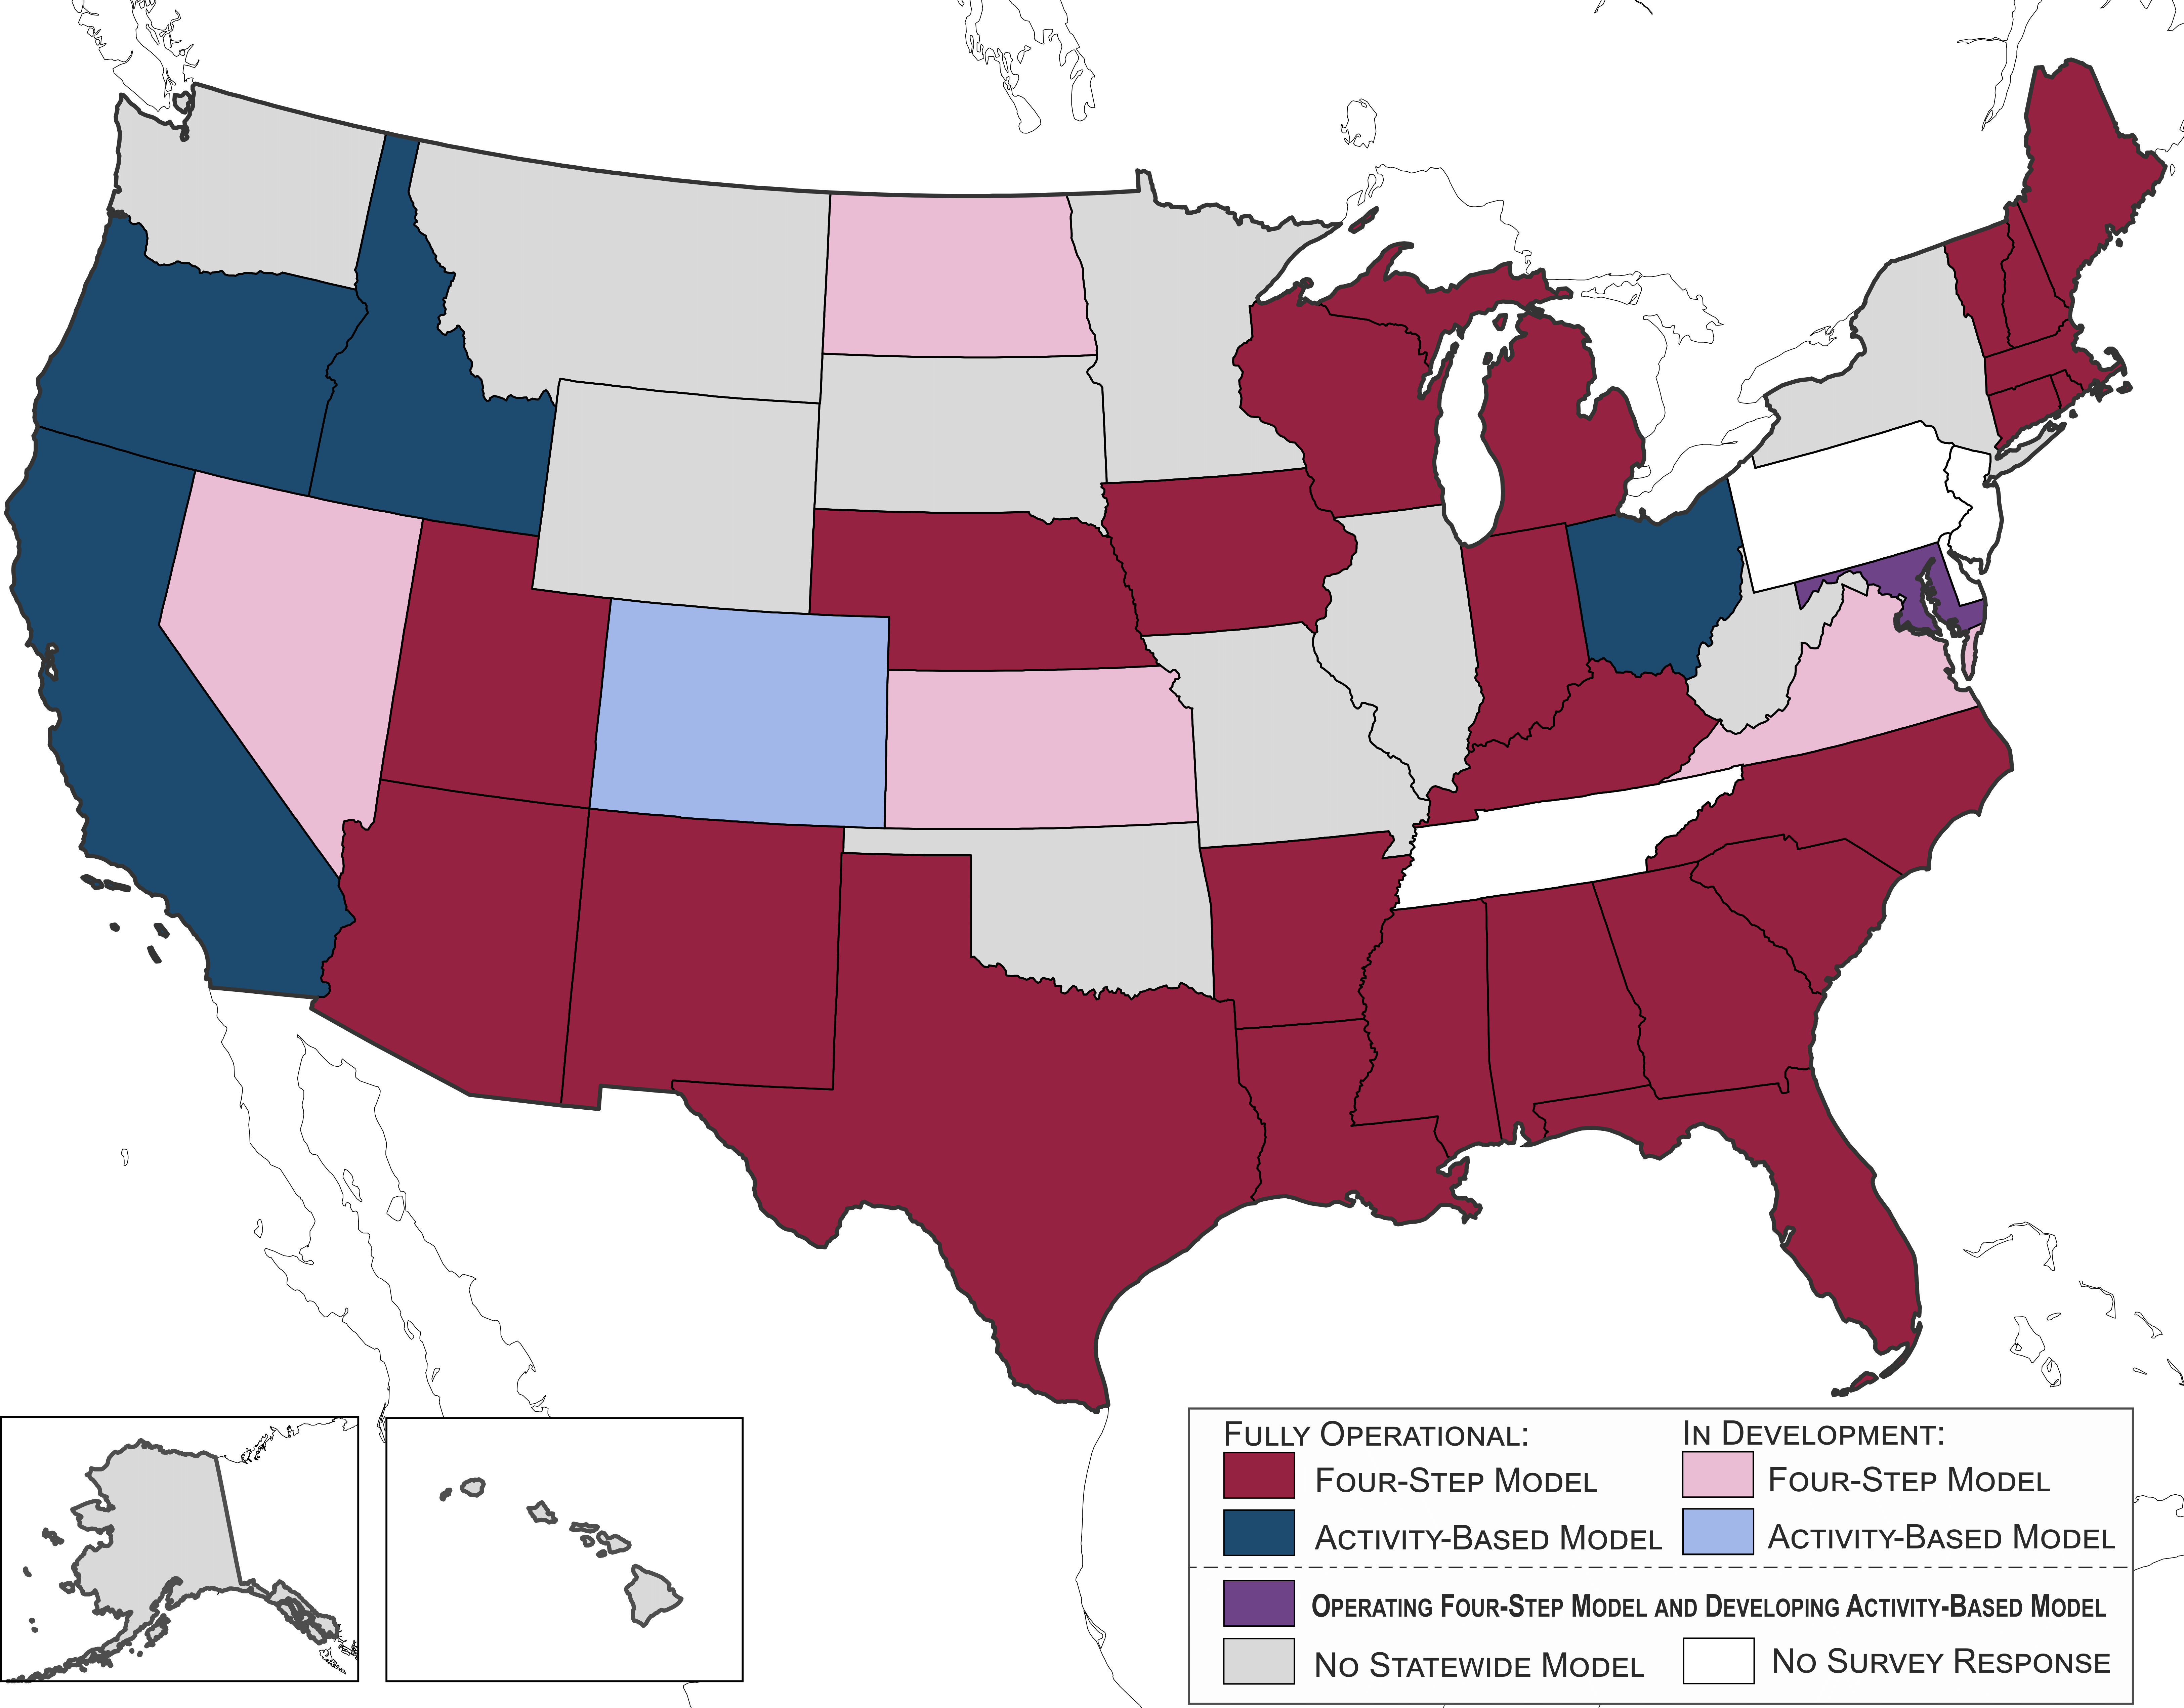
\includegraphics[width=6.5in]{graphics/06-statewide-modeling-status}
\caption{Status of statewide modeling across the U.S.}
\label{fig:statewide-modeling-status}
\end{figure}

Hawaii as an island state does not operate a statewide model. Individual models are implemented for the islands of Kauai, Maui, Oahu and Hawaii, covering over 99 percent of the state's population. Other states without statewide models tend to be clustered towards the northern part of the country in regions with lower population densities and less severe levels of congestion, which probably has affected the need and desire for developing statewide models.

The frequency of trip and tour generation methods is shown in Figure \ref{fig:person-generation-methods}. As expected, using trip rates based on cross-classification is the most common approach. In the early years of travel demand modeling, multiple regression was the dominant approach for generating trips. In multiple regression models, trip rates are treated as continuous rather than discrete variables, which may lead to unrealistically high (or sometimes even negative) number of trips in zones with unusual household type compositions. Therefore, the 1970s marked a shift away from aggregate zonal level regression analysis to more disaggregate household cross-classification procedures \citep{ortuzar11}. However, trip rates based on multiple regression have the advantage of allowing the analyst to consider multiple independent variables, and may work well if resulting generated trips are reviewed carefully for inconsistencies. Kansas and Vermont are even using both methods in trip generation.

\begin{figure}  % 7
\centering
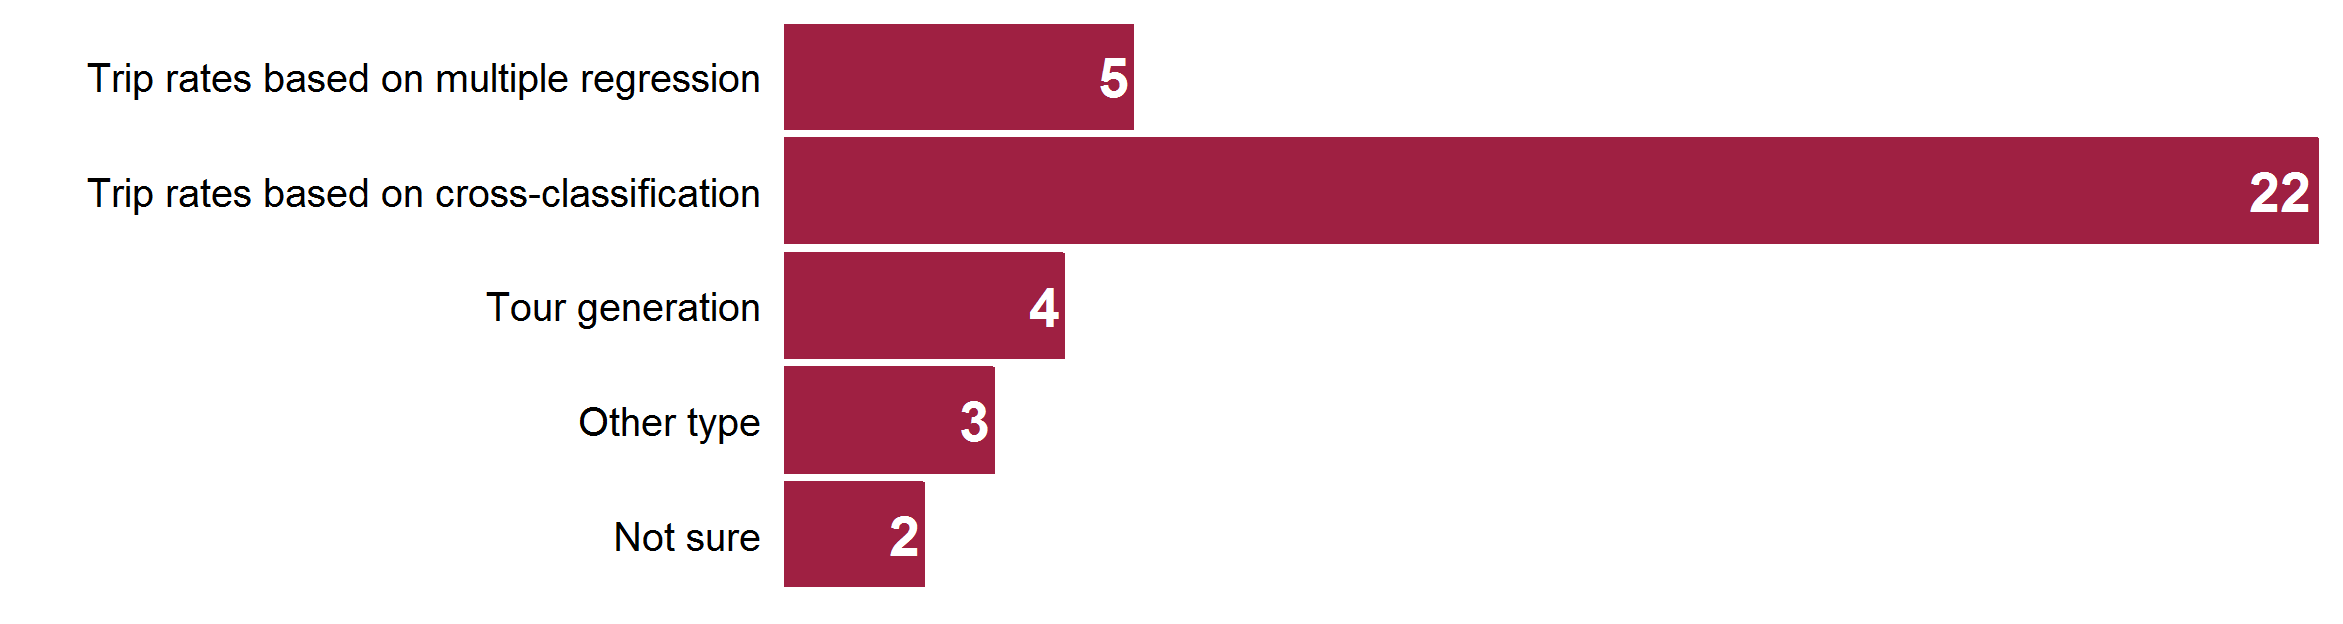
\includegraphics[width=6.4in]{graphics/07-person-generation-methods}
\caption[Frequency of trip and tour generation methods for person travel]{Frequency of trip and tour generation methods for person travel (multiple answers allowed)}
\label{fig:person-generation-methods}
\end{figure}

The fact that cross-classification rates dominate statewide modeling merely reflects the dominance of this approach in the travel demand modeling domain. Colorado models daily activity patterns (as is typically done in activity-based models), and Virginia combines logit models with regression analysis.

Trip distribution shows a strong concentration on gravity models, with 22 states applying this concept (see Figure \ref{fig:person-distribution-models}). This traditional form of trip distribution is borrowed from the physics gravity concept, explaining that the number of trips between two zones is proportional to their size (in terms of population, employment, or the number of trips generated/attracted) and inversely proportional to their distance. This model type is easy to implement and very easy to calibrate, as --- in its simplest form --- only one impedance parameter needs to be adjusted until the observed average trip length is matched by the model. However, if trips with longer distances (such as trips over 50 miles) are included, gravity models become challenging to calibrate because the tail of longer trip lengths cannot be fine-tuned very well in a gravity model with only one impedance parameter. This is less of a concern if a separate long-distance model is used (true for seven states that implemented gravity models for short-distance travel only.

\begin{figure}  % 8
\centering
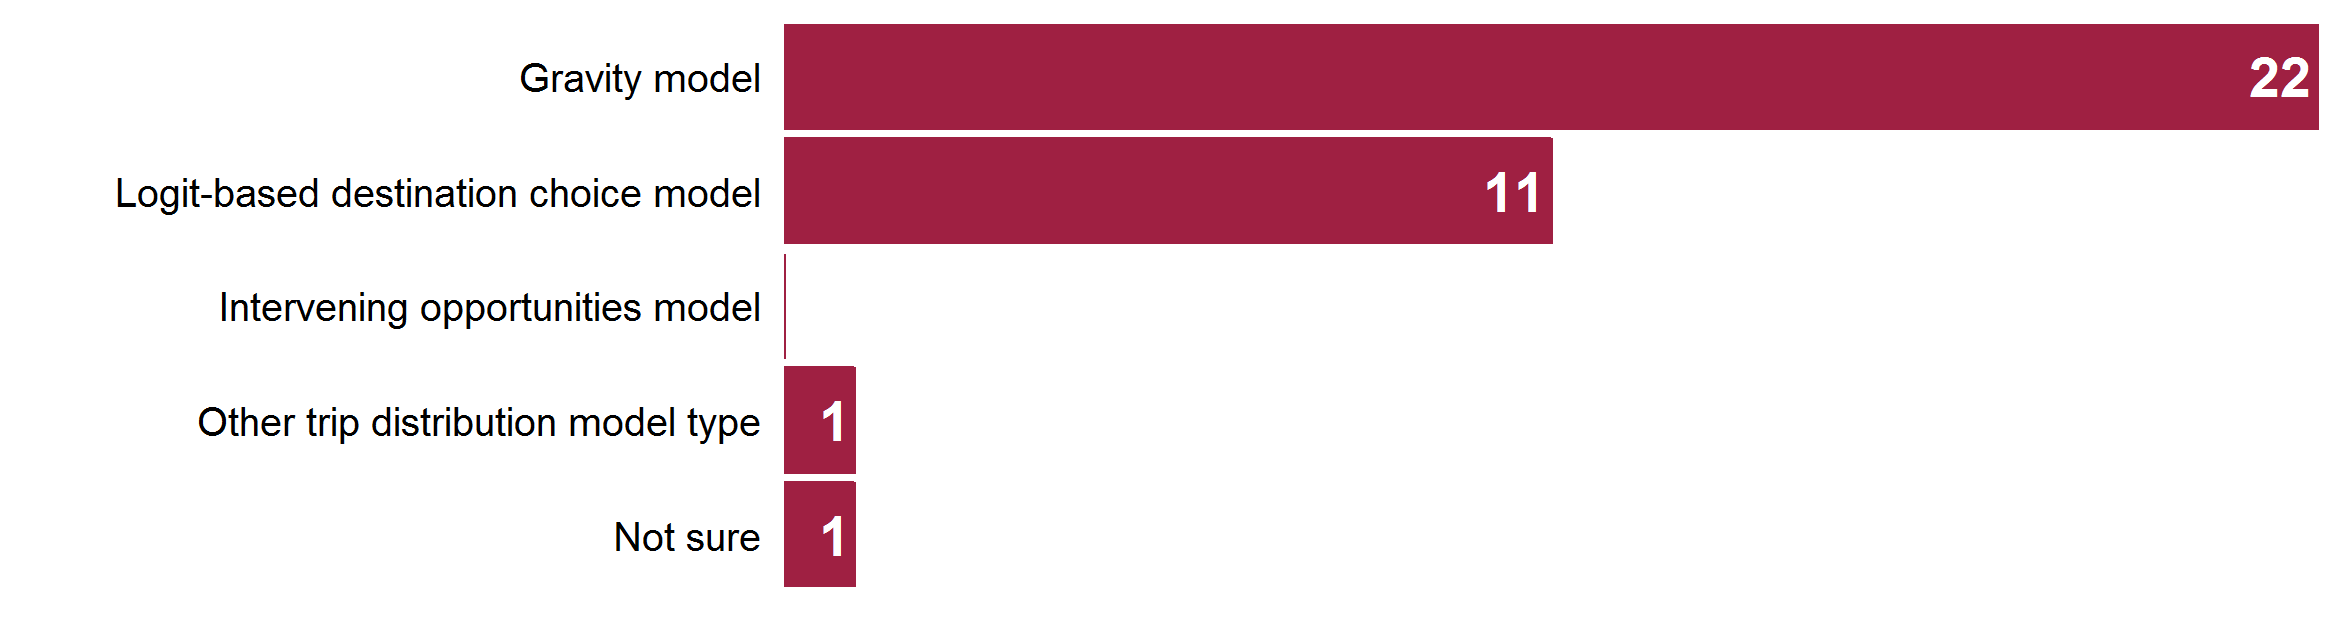
\includegraphics[width=6.4in]{graphics/08-person-distribution-models}
\caption[Frequency of trip distribution models for person travel]{Frequency of trip distribution models for person travel (multiple answers allowed)}
\label{fig:person-distribution-models}
\end{figure}

The logit-based destination choice model, on the other hand, evaluates different destinations against each other, taking into account the attraction in every other zone (measured by socio-economic data or the number of trips attracted), the distance to every other zone, and possibly other factors that may affect destination choice. In the Maryland statewide model, for example, an additional penalty was used to reflect the observed psychological barrier of choosing destinations on the other side of major rivers. 

As shown in Figure \ref{fig:person-distribution-models}, eleven states apply logit-based destination choice models. This includes Ohio, where a logit-based destination choice model is joined with an economic allocation model for work locations. Even though logit-based destination choice models are capable of handling long-distance trips, eight out of eleven states that use logit-based destination choice models have also implemented a separate long-distance travel model. Such a combination commonly ensures the largest model sensitivities for the trip distribution step.

Note that no state is using an intervening opportunities model \citep{stouffer40}, a concept from social sciences that received attention in the 1960s but is no longer common in travel demand modeling.

While early travel demand models ignored mode choice entirely, nowadays about every other statewide model explicitly accounts for mode selection, as shown in Figure \ref{fig:person-mode-choice}. Thirteen states responded that they only generate auto trips, obviating the need for a mode choice model. Furthermore, five states apply static (fixed) modal shares, making it 18 states (or 53 percent) that do not model mode choice. Of the 16 states that do model mode choice, the clear majority use nested logit models, with only two states using simple multinomial formulations. Probit and mixed logit models, sometimes applied in urban travel demand models, are not in use for mode choice modeling in statewide models in the U.S.

\begin{figure}
\centering
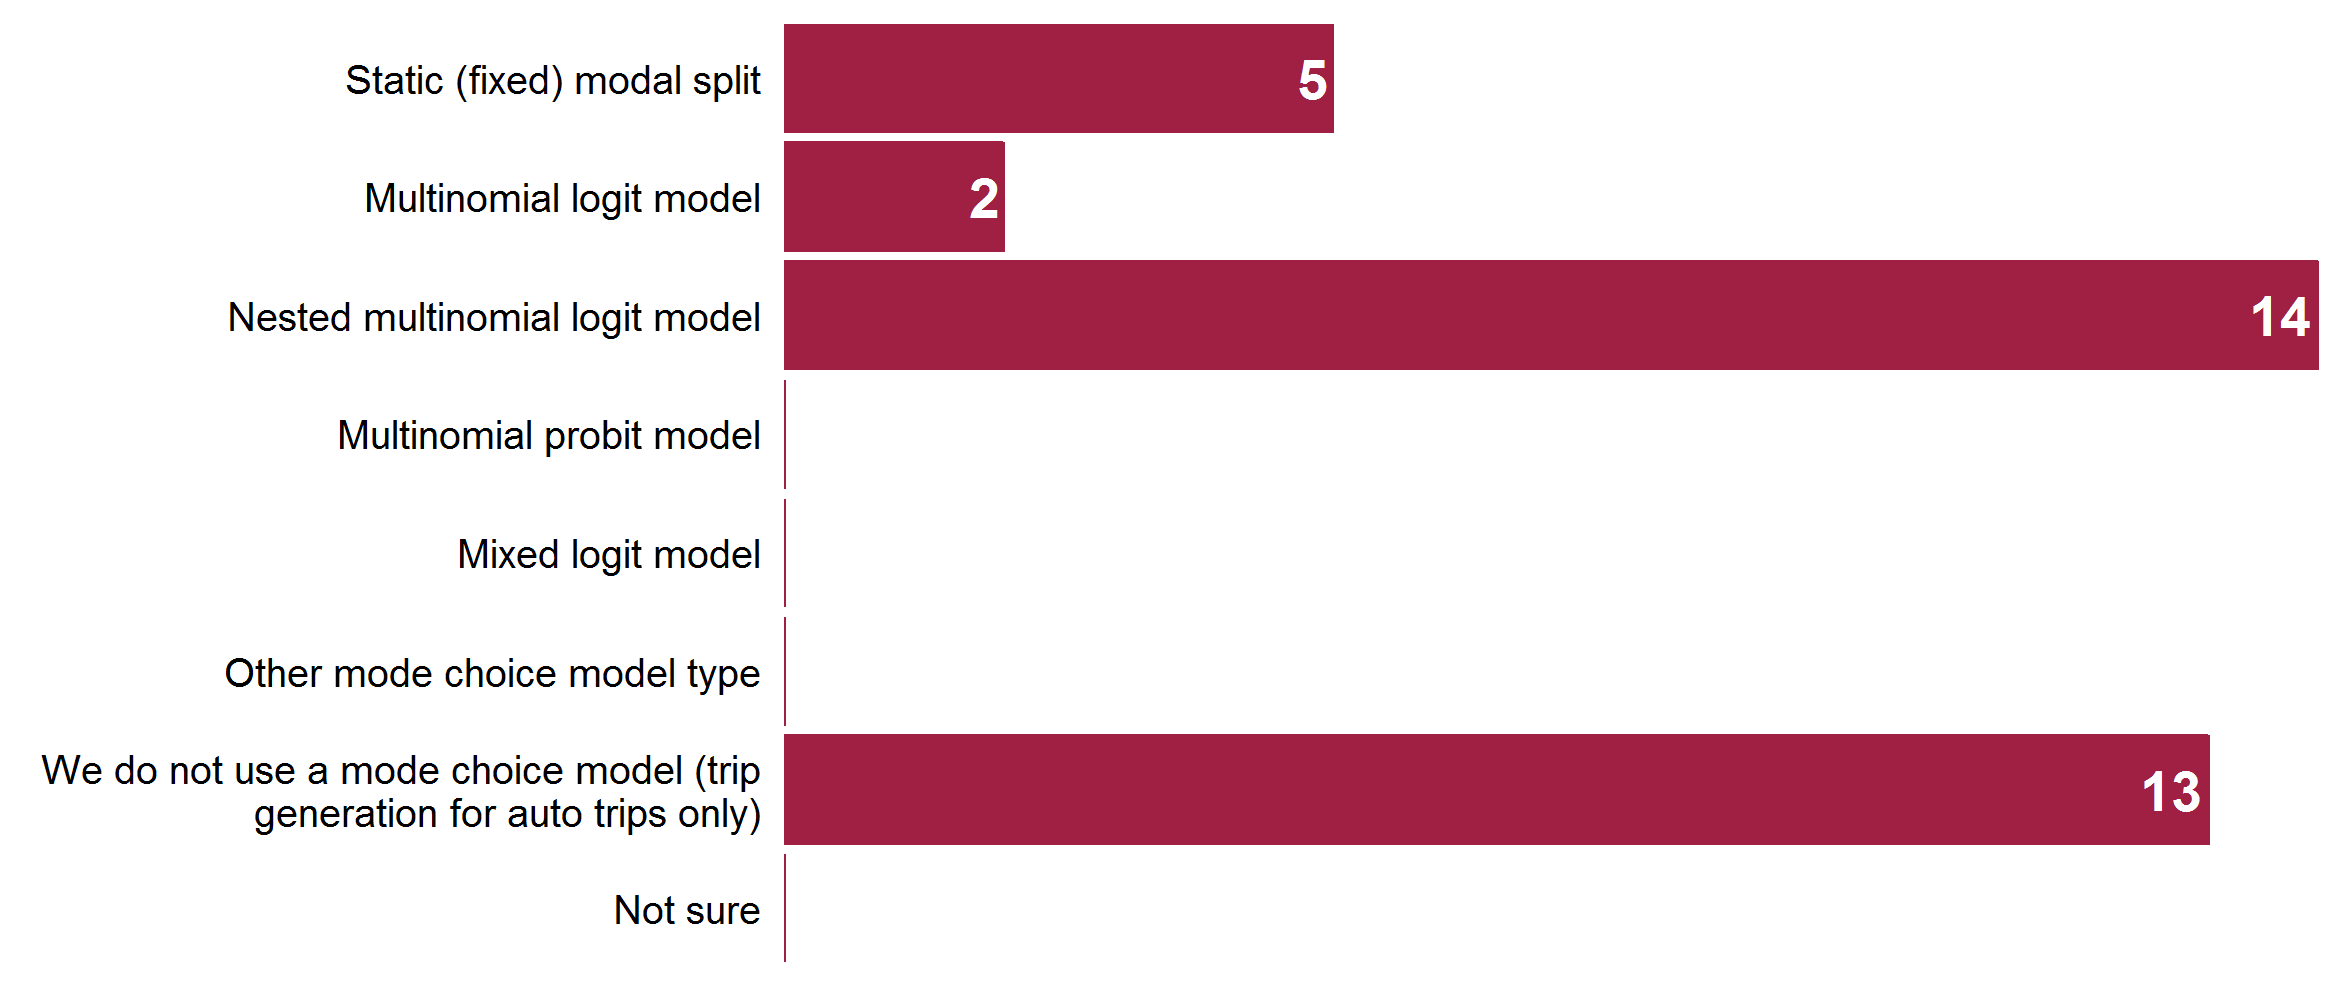
\includegraphics[width=6.4in]{graphics/09-person-mode-choice}
\caption{Frequency of mode choice models for person travel}
\label{fig:person-mode-choice}
\end{figure}

It should be noted that three of the states that do not model mode choice for short-distance travel do so for long-distance trips (North Carolina, Virginia, and Wisconsin). Nevertheless, it is remarkable that many statewide models ignore mode choice. While most scenarios analyzed with statewide models refer to changes of the highway network (see \S\ref{sec:scenario-analysis}), impacts on mode choice may be significant. Increased congestion or higher gas prices are likely to push some travelers from the auto to the transit mode, and vice versa, congestion relief through additional roadway construction may trigger transit riders to switch to the car. This outcome is missed in models without an explicit mode choice model, although possibly less important in non-MPO areas with limited transit options.

The modes of transportation represented in statewide models for person travel are shown in Figure \ref{fig:person-modes-represented}. This graphic includes statewide models that apply static mode shares and mode choice models. All statewide models include auto trips as the dominant mode, analyses of which such models are built for. Thirteen of them distinguish auto occupancy, at least between drive-alone and share-ride. Indiana and Maine split trucks from person travel in the mode choice model, which means (a) that truck trip generation rates were added to person trip generation rates and (b) that the same trip distribution was applied for person travel and trucks. Virginia aggregates all transit modes into one choice for transit. Colorado has a separate mode for school buses.

\begin{figure}  % 10
\centering
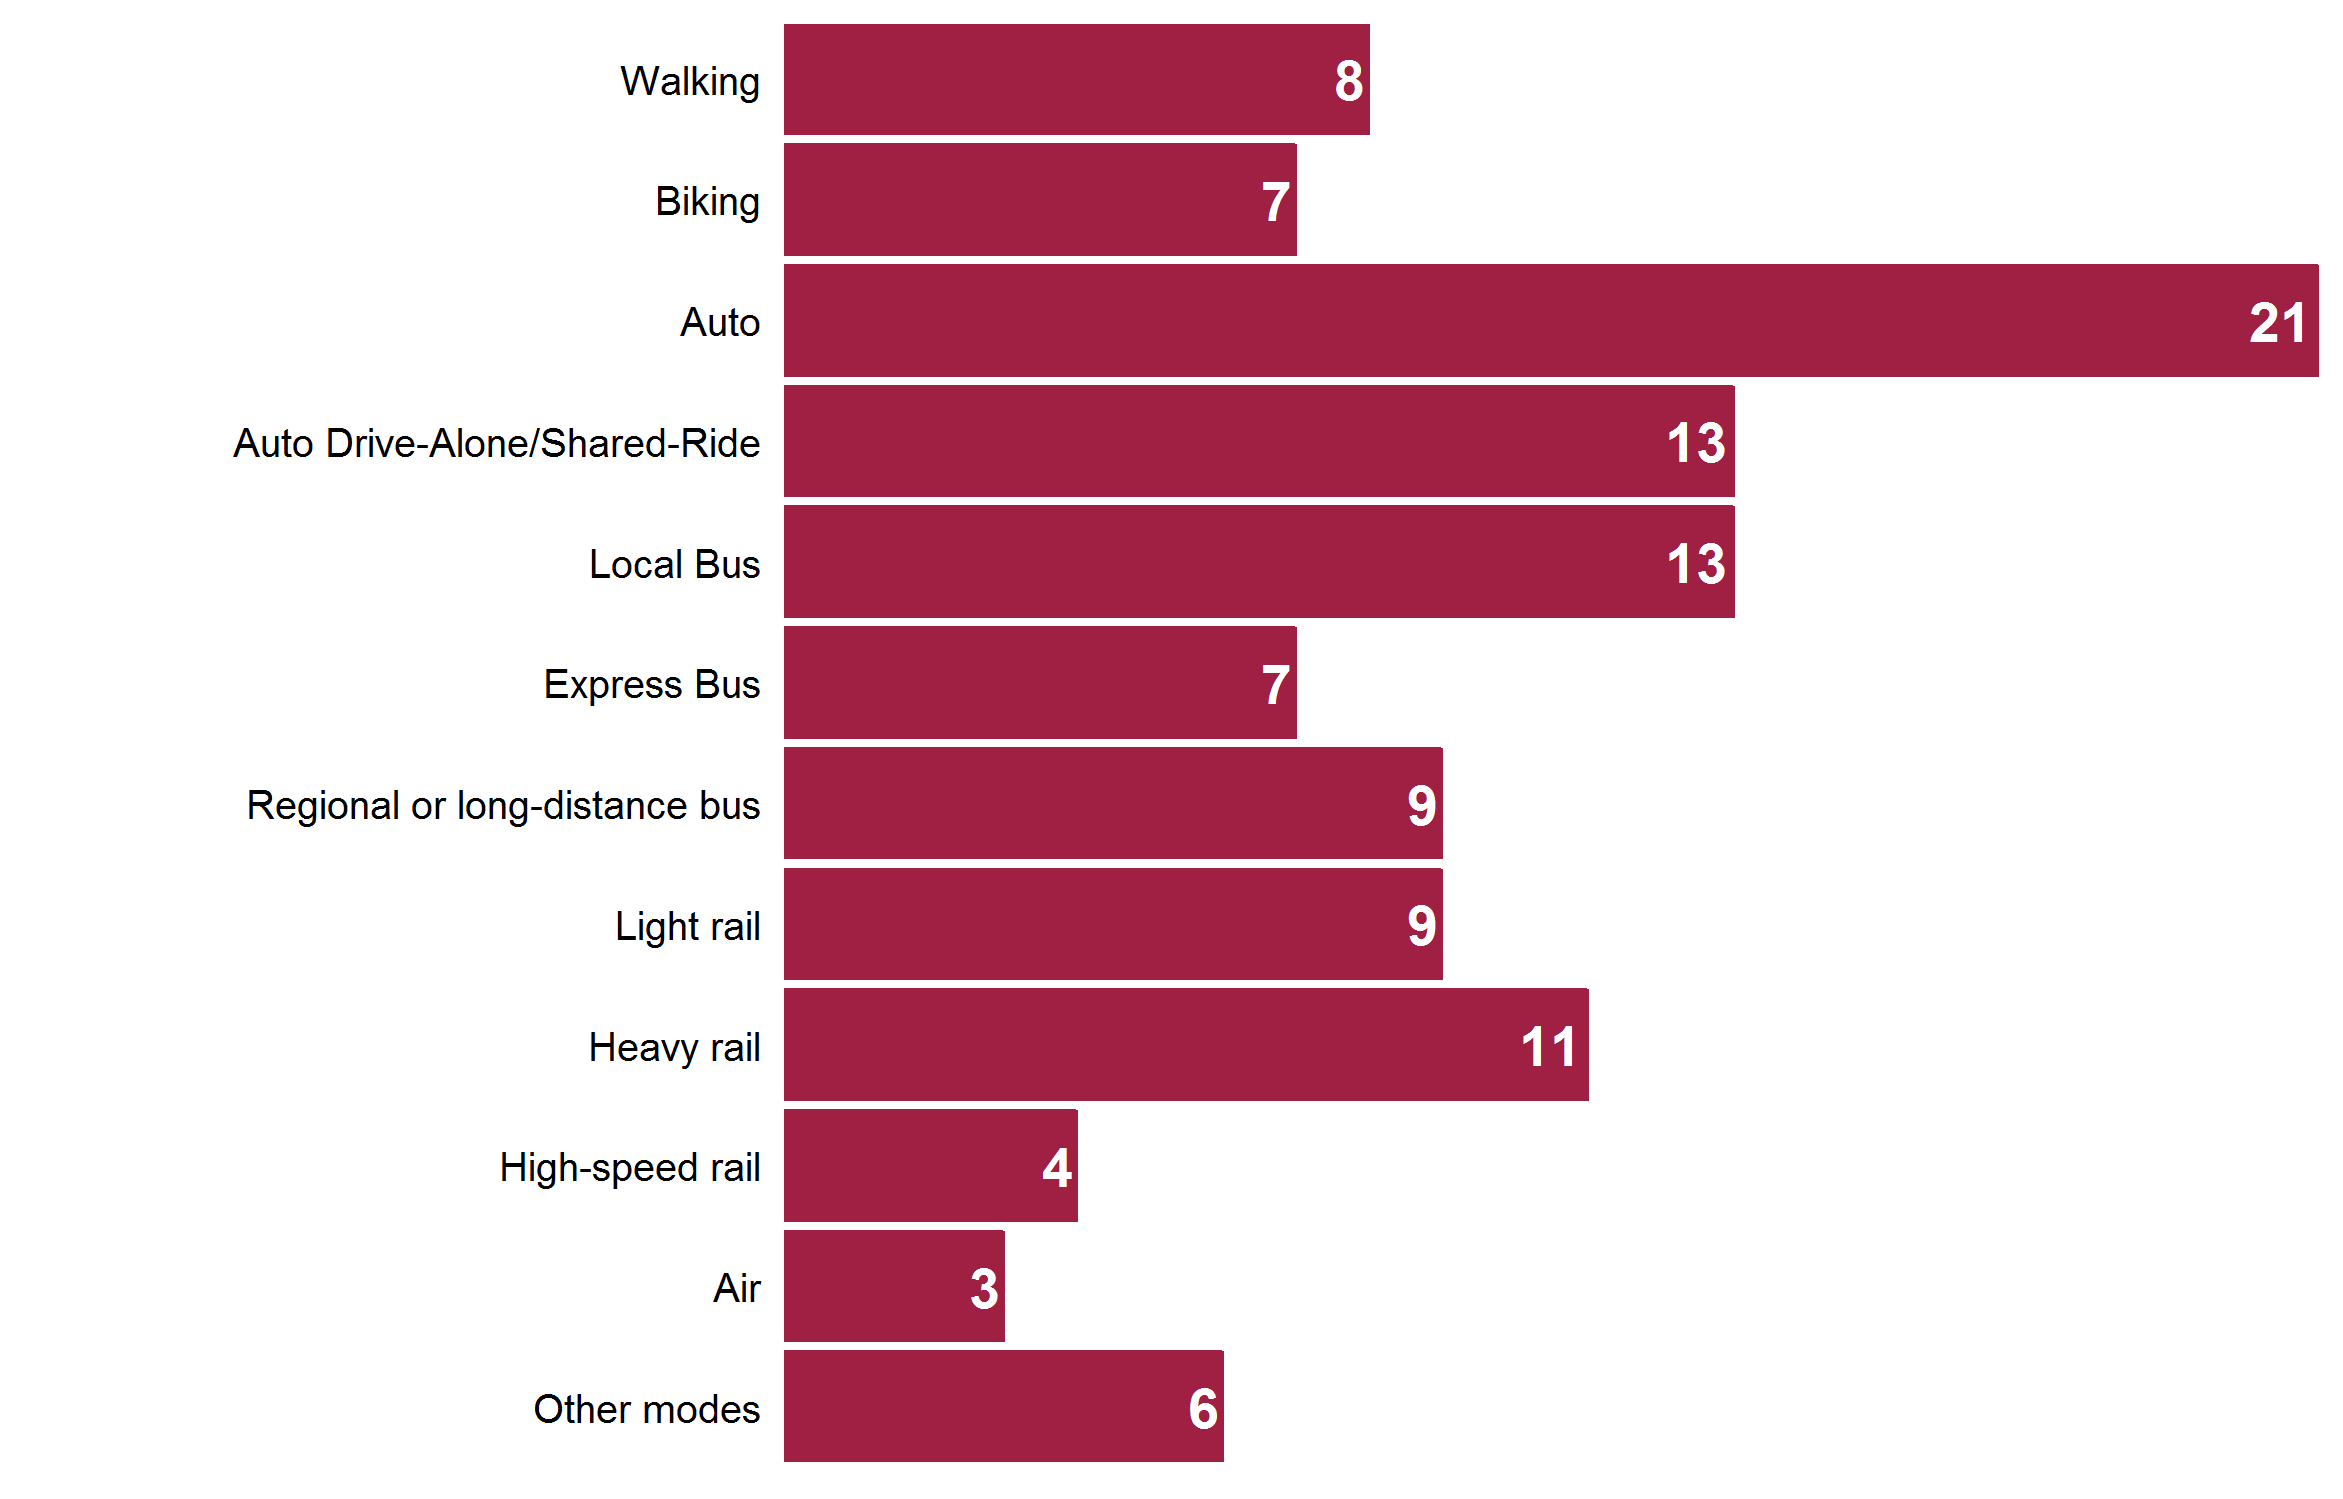
\includegraphics[width=6.4in]{graphics/10-person-modes-represented}
\caption[Modes represented in mode choice models for person travel]{Modes represented in mode choice models for person travel (multiple answers allowed)}
\label{fig:person-modes-represented}
\end{figure}

Eight models account for non-motorized travel as well. Often, the resolution in statewide models is too coarse to reasonably account for this mode. However, given the rising interest in non-motorized modes as an alternative to auto travel and for population health analyses, it is encouraging that almost a quarter of all statewide models account for them.

Local bus is the most frequently modeled transit mode, followed by heavy rail (which commonly includes commuter rail), regional or long-distance buses and light rail. High-speed rail is explicitly accounted for in the statewide models of California, Iowa, Maryland and Texas. Air travel is explicitly represented in the Florida, Oregon, and Texas models. However, the latter two have explicit long-distance models, where these modes most likely are handled.

The period of day that travel occurs within is represented in 12 out of 34 states (35 percent), as shown in Figure \ref{fig:time-of-day}. Note that this time-of-day separation applies to all traffic markets that are assigned to the highway network, including short and long-distance travel as well as person and freight trips. Congestion is found predominantly during peak hours, which is why many four-step models have added a fifth step to split the travel demand into a selected number of time-of-day periods. This way, congestion might be severe in the morning peak hours and cause travelers to switch to transit or choose detours to avoid bottlenecks, while during the mid-day period traffic could be comparatively light. Rural states with very low levels of congestion may omit this step, as travel time will not differ significantly by time of day.

\begin{figure}   % 11
\centering
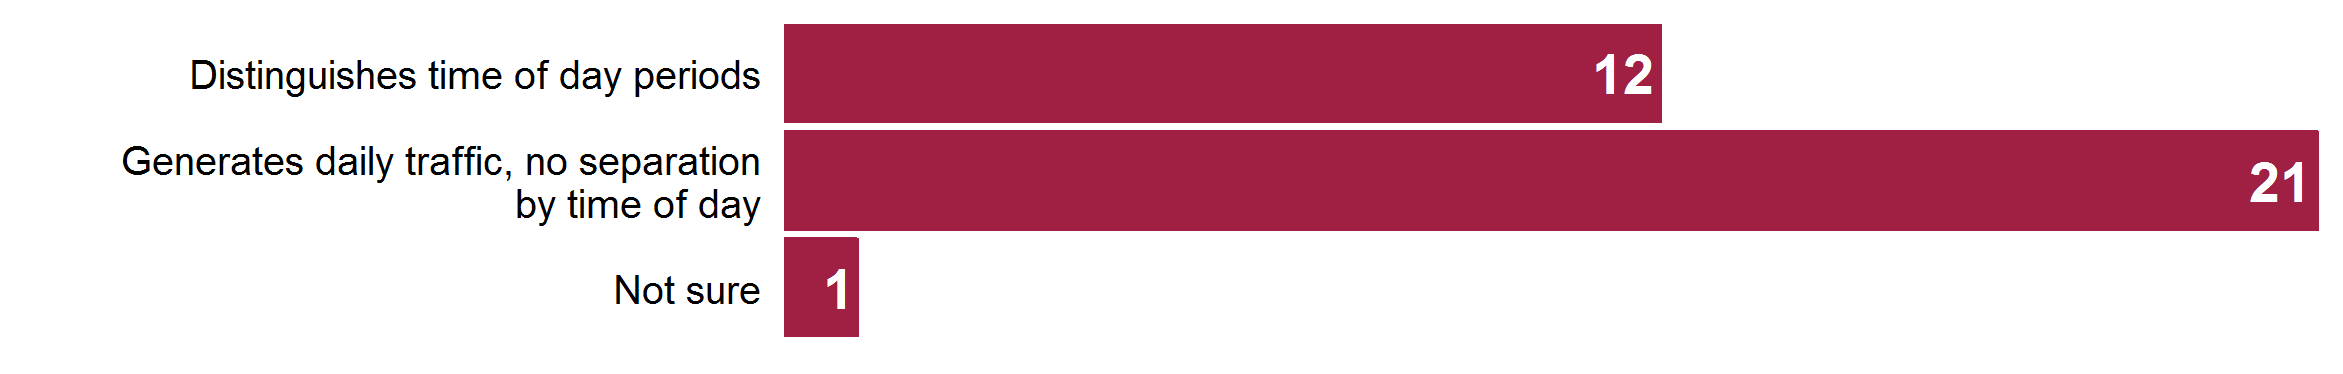
\includegraphics[width=6.4in]{graphics/11-time-of-day}
\caption{Time of day representation in statewide models}
\label{fig:time-of-day}
\end{figure}

The number of time-of-day periods distinguished by individual models is shown in Figure \ref{fig:time-periods-represented}. Most models deal with four time periods, usually defined as AM Peak, Midday, PM Peak and Night. Colorado is developing their model and intends to distinguish 7-10 periods. In general, a more fine-grained resolution of time is desirable. This will enable a model to represent better the time-dependent effects of congestion, which some travelers will attempt to avoid by traveling before or after those periods. However, more time intervals increase the computational burden and the need to model departure time shifts.

\begin{figure}[!bt]   % 12
\centering
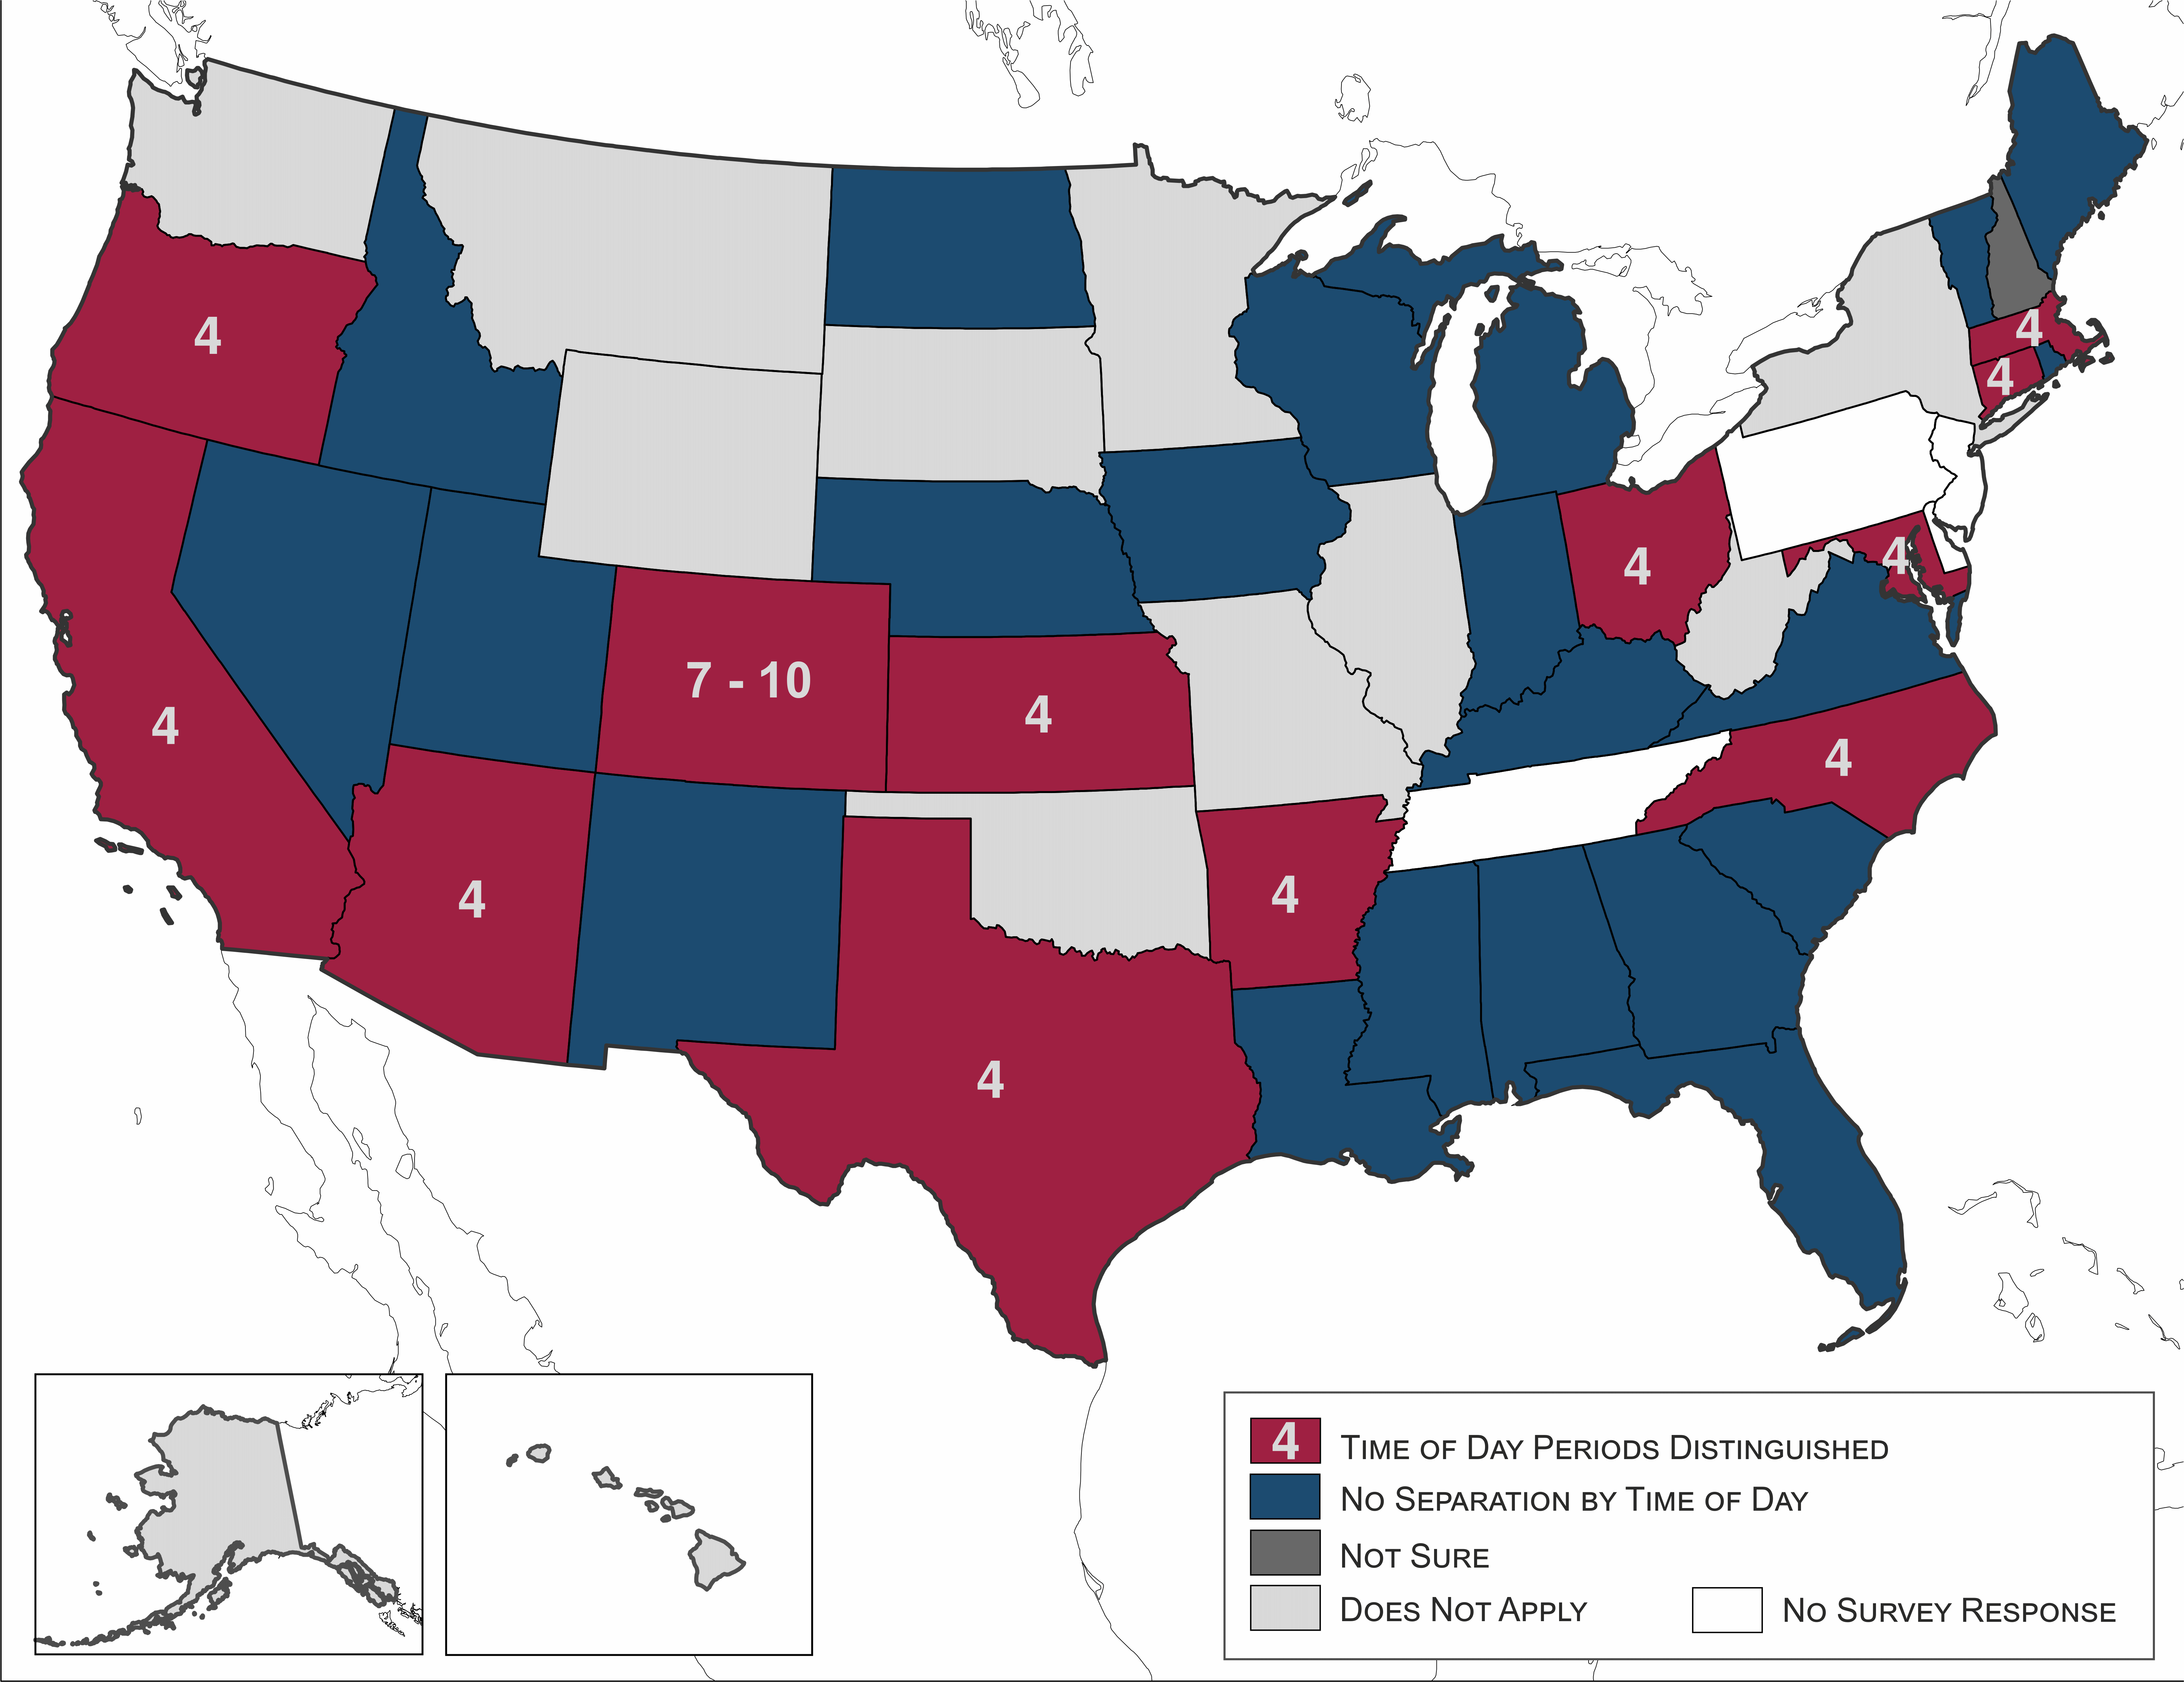
\includegraphics[width=6.5in]{graphics/12-time-periods-represented}
\caption{Number of time periods distinguished by individual statewide models}
\label{fig:time-periods-represented}
\end{figure}

Colorado, Ohio, and Oregon reported that their models generated travel demand in finer increments, representing 24 time-of-day periods in travel demand for Colorado and 19 for Ohio and Oregon. Due to runtime limitations, none of these models assigns all 24 or 19 time-or-day periods to the network (which was asked about in the responses shown in Figure \ref{fig:time-periods-represented}). However, those three models offer the ability to analyze travel demand in finer time intervals.

Four out of five statewide models use the traditional static user equilibrium algorithm for the assignment of highway travel, as shown in Figure \ref{fig:assignment-algorithms}. Alabama, Nebraska, and North Dakota apply the all-or-nothing assignment, presumably because intercity congestion in these states is very light and congested travel times does not differ much from free-flow travel times. Kansas uses a stochastic user equilibrium, and Maine applies an incremental capacity constraint model. Note that the assignment applies to all traffic markets that are assigned to the highway network, including short and long-distance travel as well as person and freight trips.

\begin{figure}   % 13
\centering
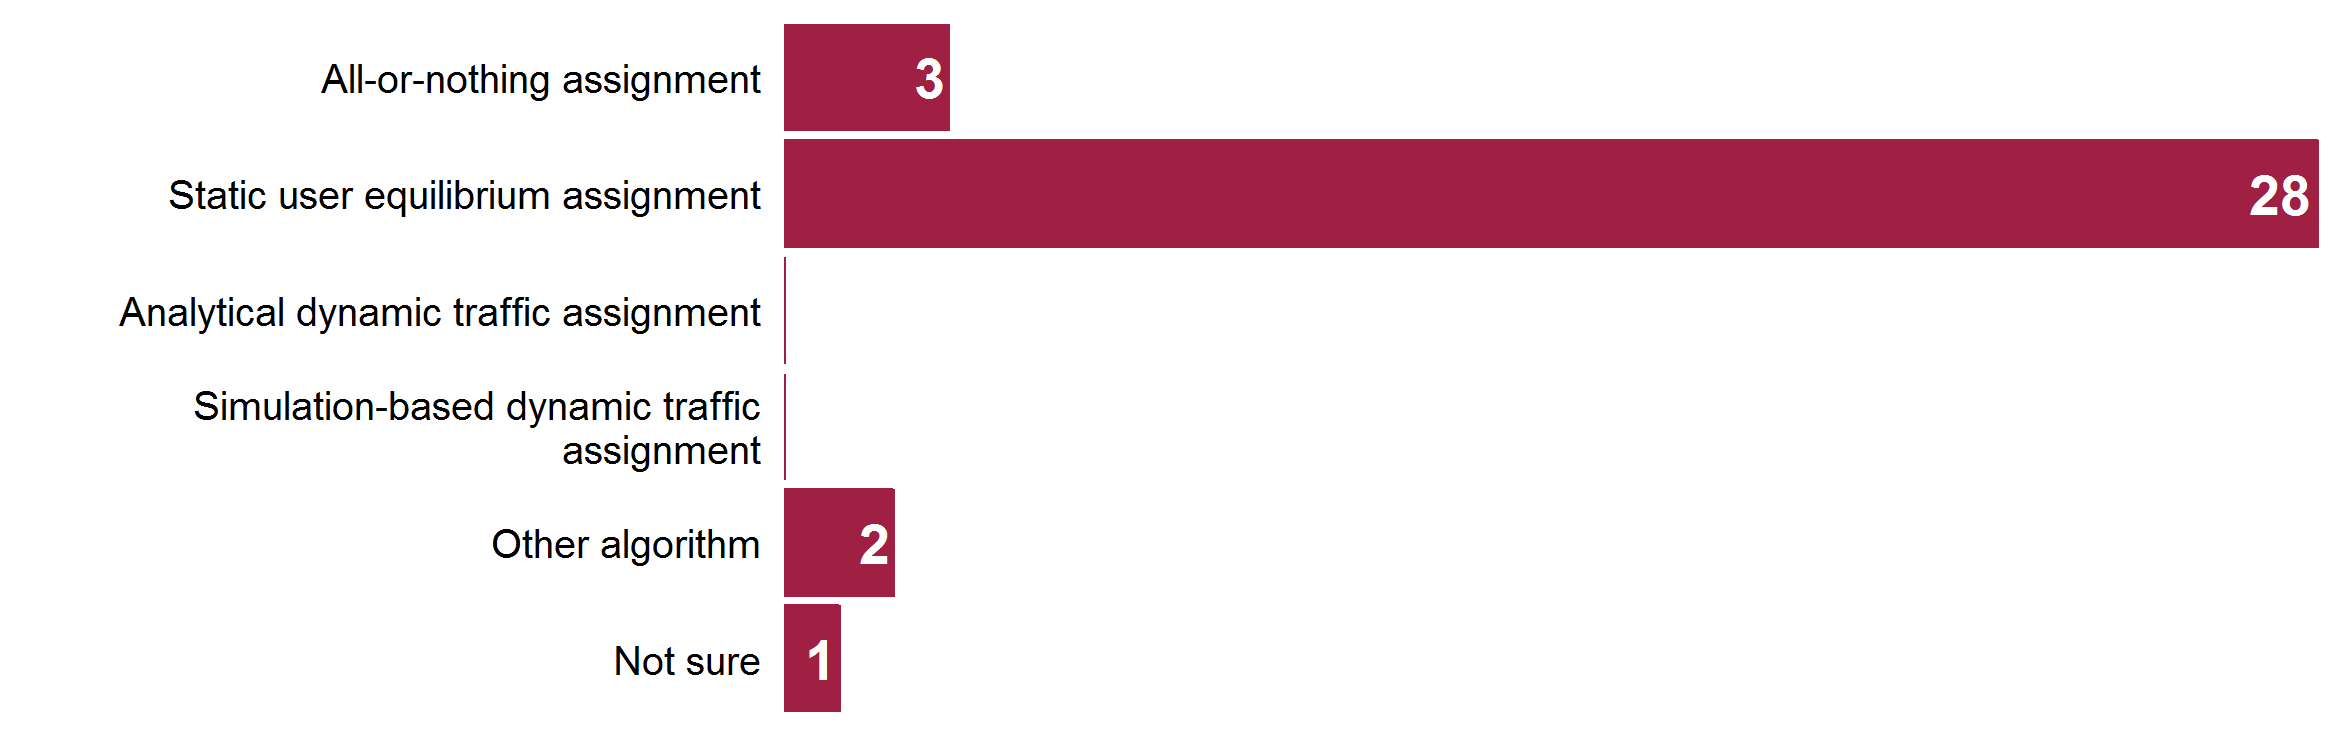
\includegraphics[width=6.4in]{graphics/13-assignment-algorithm}
\caption{Frequency of assignment algorithms in statewide models}
\label{fig:assignment-algorithms}
\end{figure}

Some models provide feedback from the assignment back to previous steps of the model. For example, under congested conditions some travelers may choose other destinations or other modes. By feeding back travel times to previous steps, an equilibrium between different submodules and congested travel times may be reached. The concept is shown for traditional four-step models in Figure \ref{fig:trip-based-feedback}. Feedback of congested travel times may also be provided for person long-distance travel and freight flows.

\begin{figure}   % 14
\centering
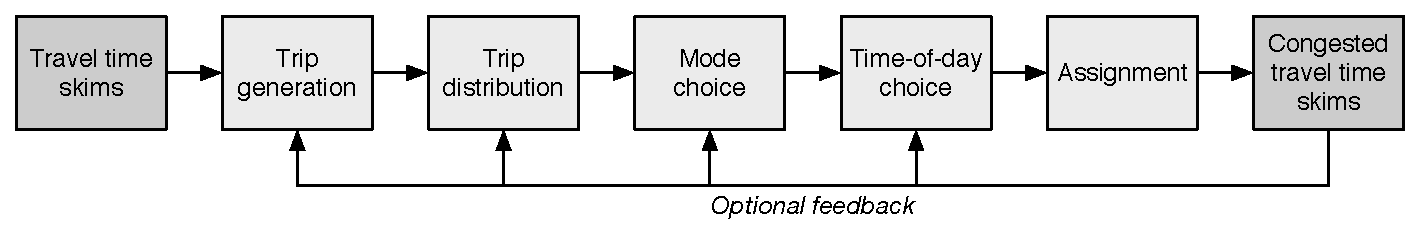
\includegraphics[width=6.4in]{graphics/14-feedback-process}
\caption{Trip-based model feedback process}
\label{fig:trip-based-feedback}
\end{figure}

Figure \ref{fig:feedback-frequency} shows how many statewide models apply feedback. Congested travel times are fed back into the trip distribution step in 20 out of 34 models (59 percent). As the mode choice model is run after the trip distribution model, presumably congested travel times affect mode choice in those models as well. Six models feed congested travel times back to trip generation.

\begin{figure}   % 15
\centering
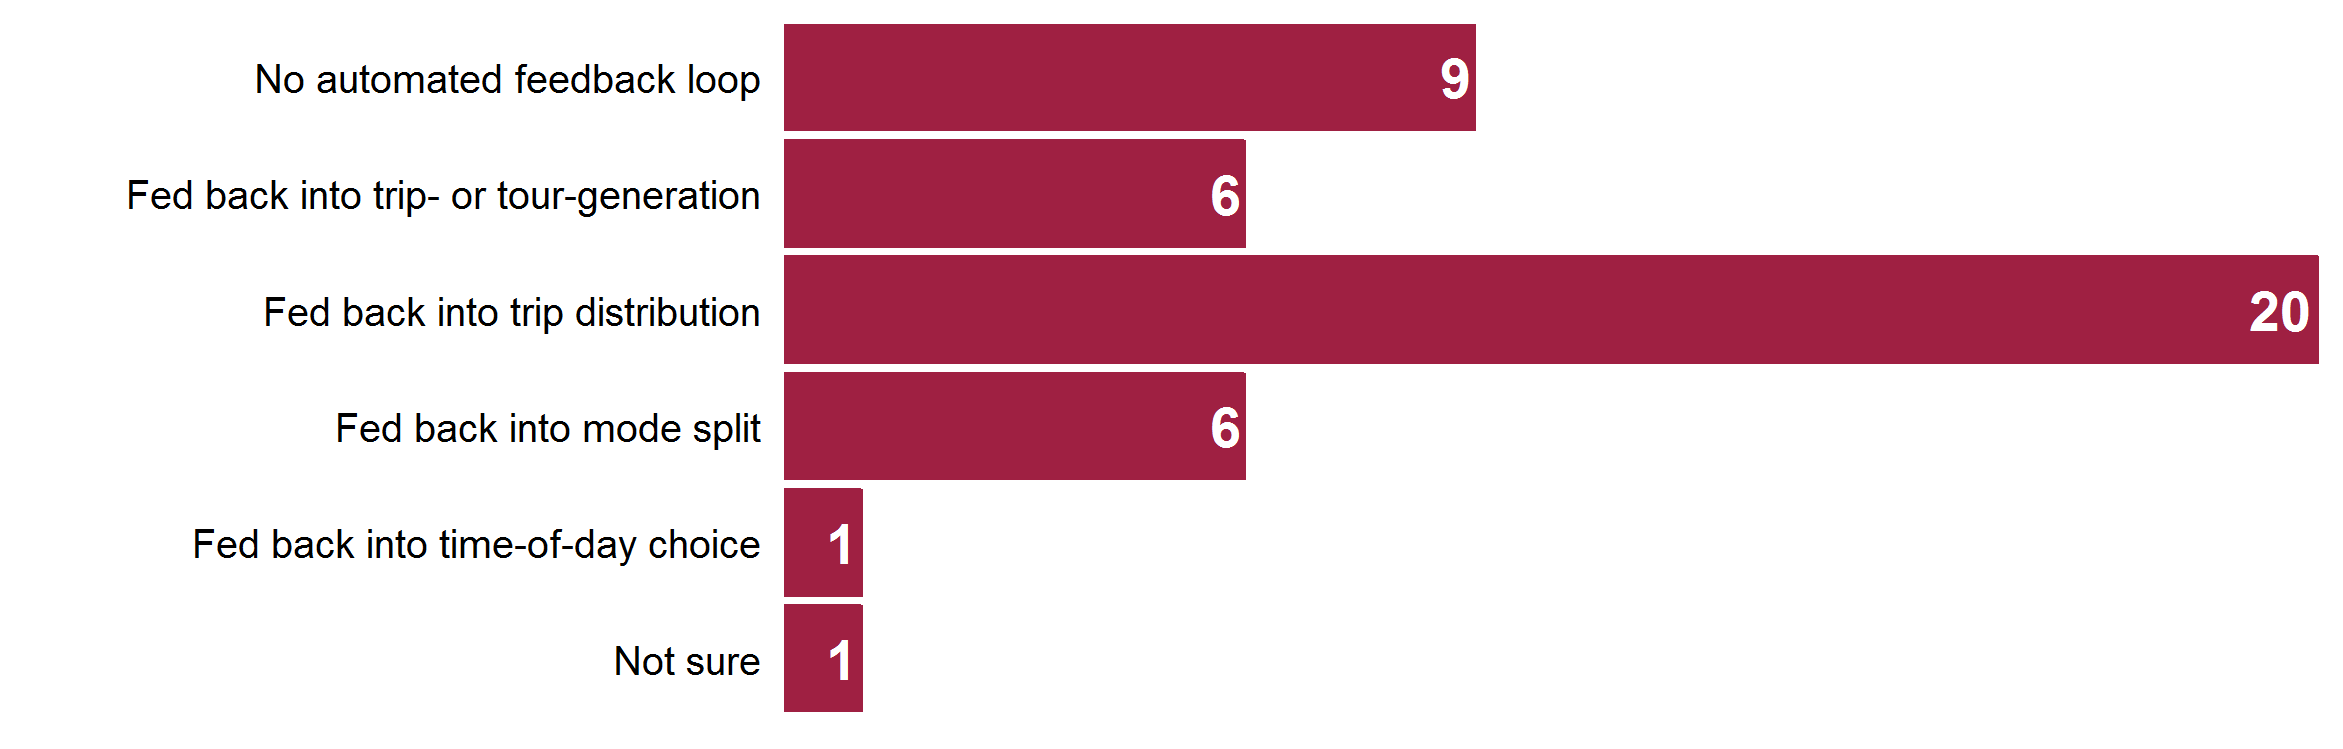
\includegraphics[width=6.4in]{graphics/15-feedback-frequency}
\caption[Frequency of feedback of congested travel times in statewide models]{Frequency of feedback of congested travel times in statewide models (multiple answers allowed)}
\label{fig:feedback-frequency}
\end{figure}

\section{Person long-distance travel}

Fifteen states (or 44 percent) have implemented explicit long-distance person travel demand models (Figure \ref{fig:person-long-distance-frequency}). No consistent definition of a long-distance trip exists, yet most states define long-distance travel as trips greater than 50 miles. This threshold is in line with the long-distance element of the 2001 NHTS survey. For Georgia, long-distance trips have been defined as 75 miles or more, for Nevada the threshold is 80 miles, and for Texas it is 150 miles. Arizona and North Carolina exclude long-distance commute trips (which are handled by the short-distance model because they are unlike most other habitual long-distance trips). For Alabama, long-distance trips are those that either cross the state boundary or travel across more than one MPO boundary, and for Colorado, trips that cross the state boundary are handled separately. Iowa is the only state that defines long-distance trips by travel time, namely greater than 60 minutes.

\begin{figure}   % 16
\centering
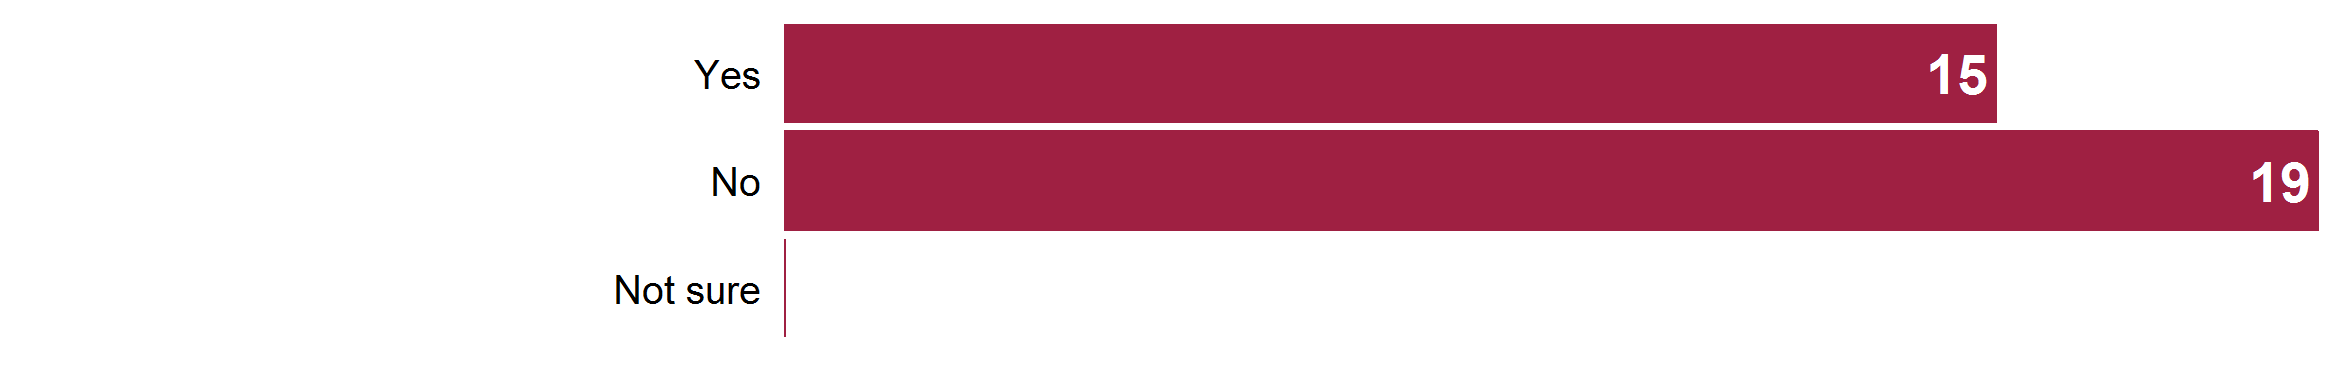
\includegraphics[width=6.4in]{graphics/16-person-long-distance-frequency}
\caption{Frequency of explicit long-distance models for person travel}
\label{fig:person-long-distance-frequency}
\end{figure}

Long-distance models tend to be implemented in larger states by area, as shown in Figure \ref{fig:person-long-distance-states}. However, some large states, such as California or Florida, do not operate long-distance models, while other smaller states, like Maryland, run long-distance models. Some states, such as Georgia, capture long-distance travel with a separate trip purpose in the short-distance travel model.

\begin{figure}   %  17
\centering
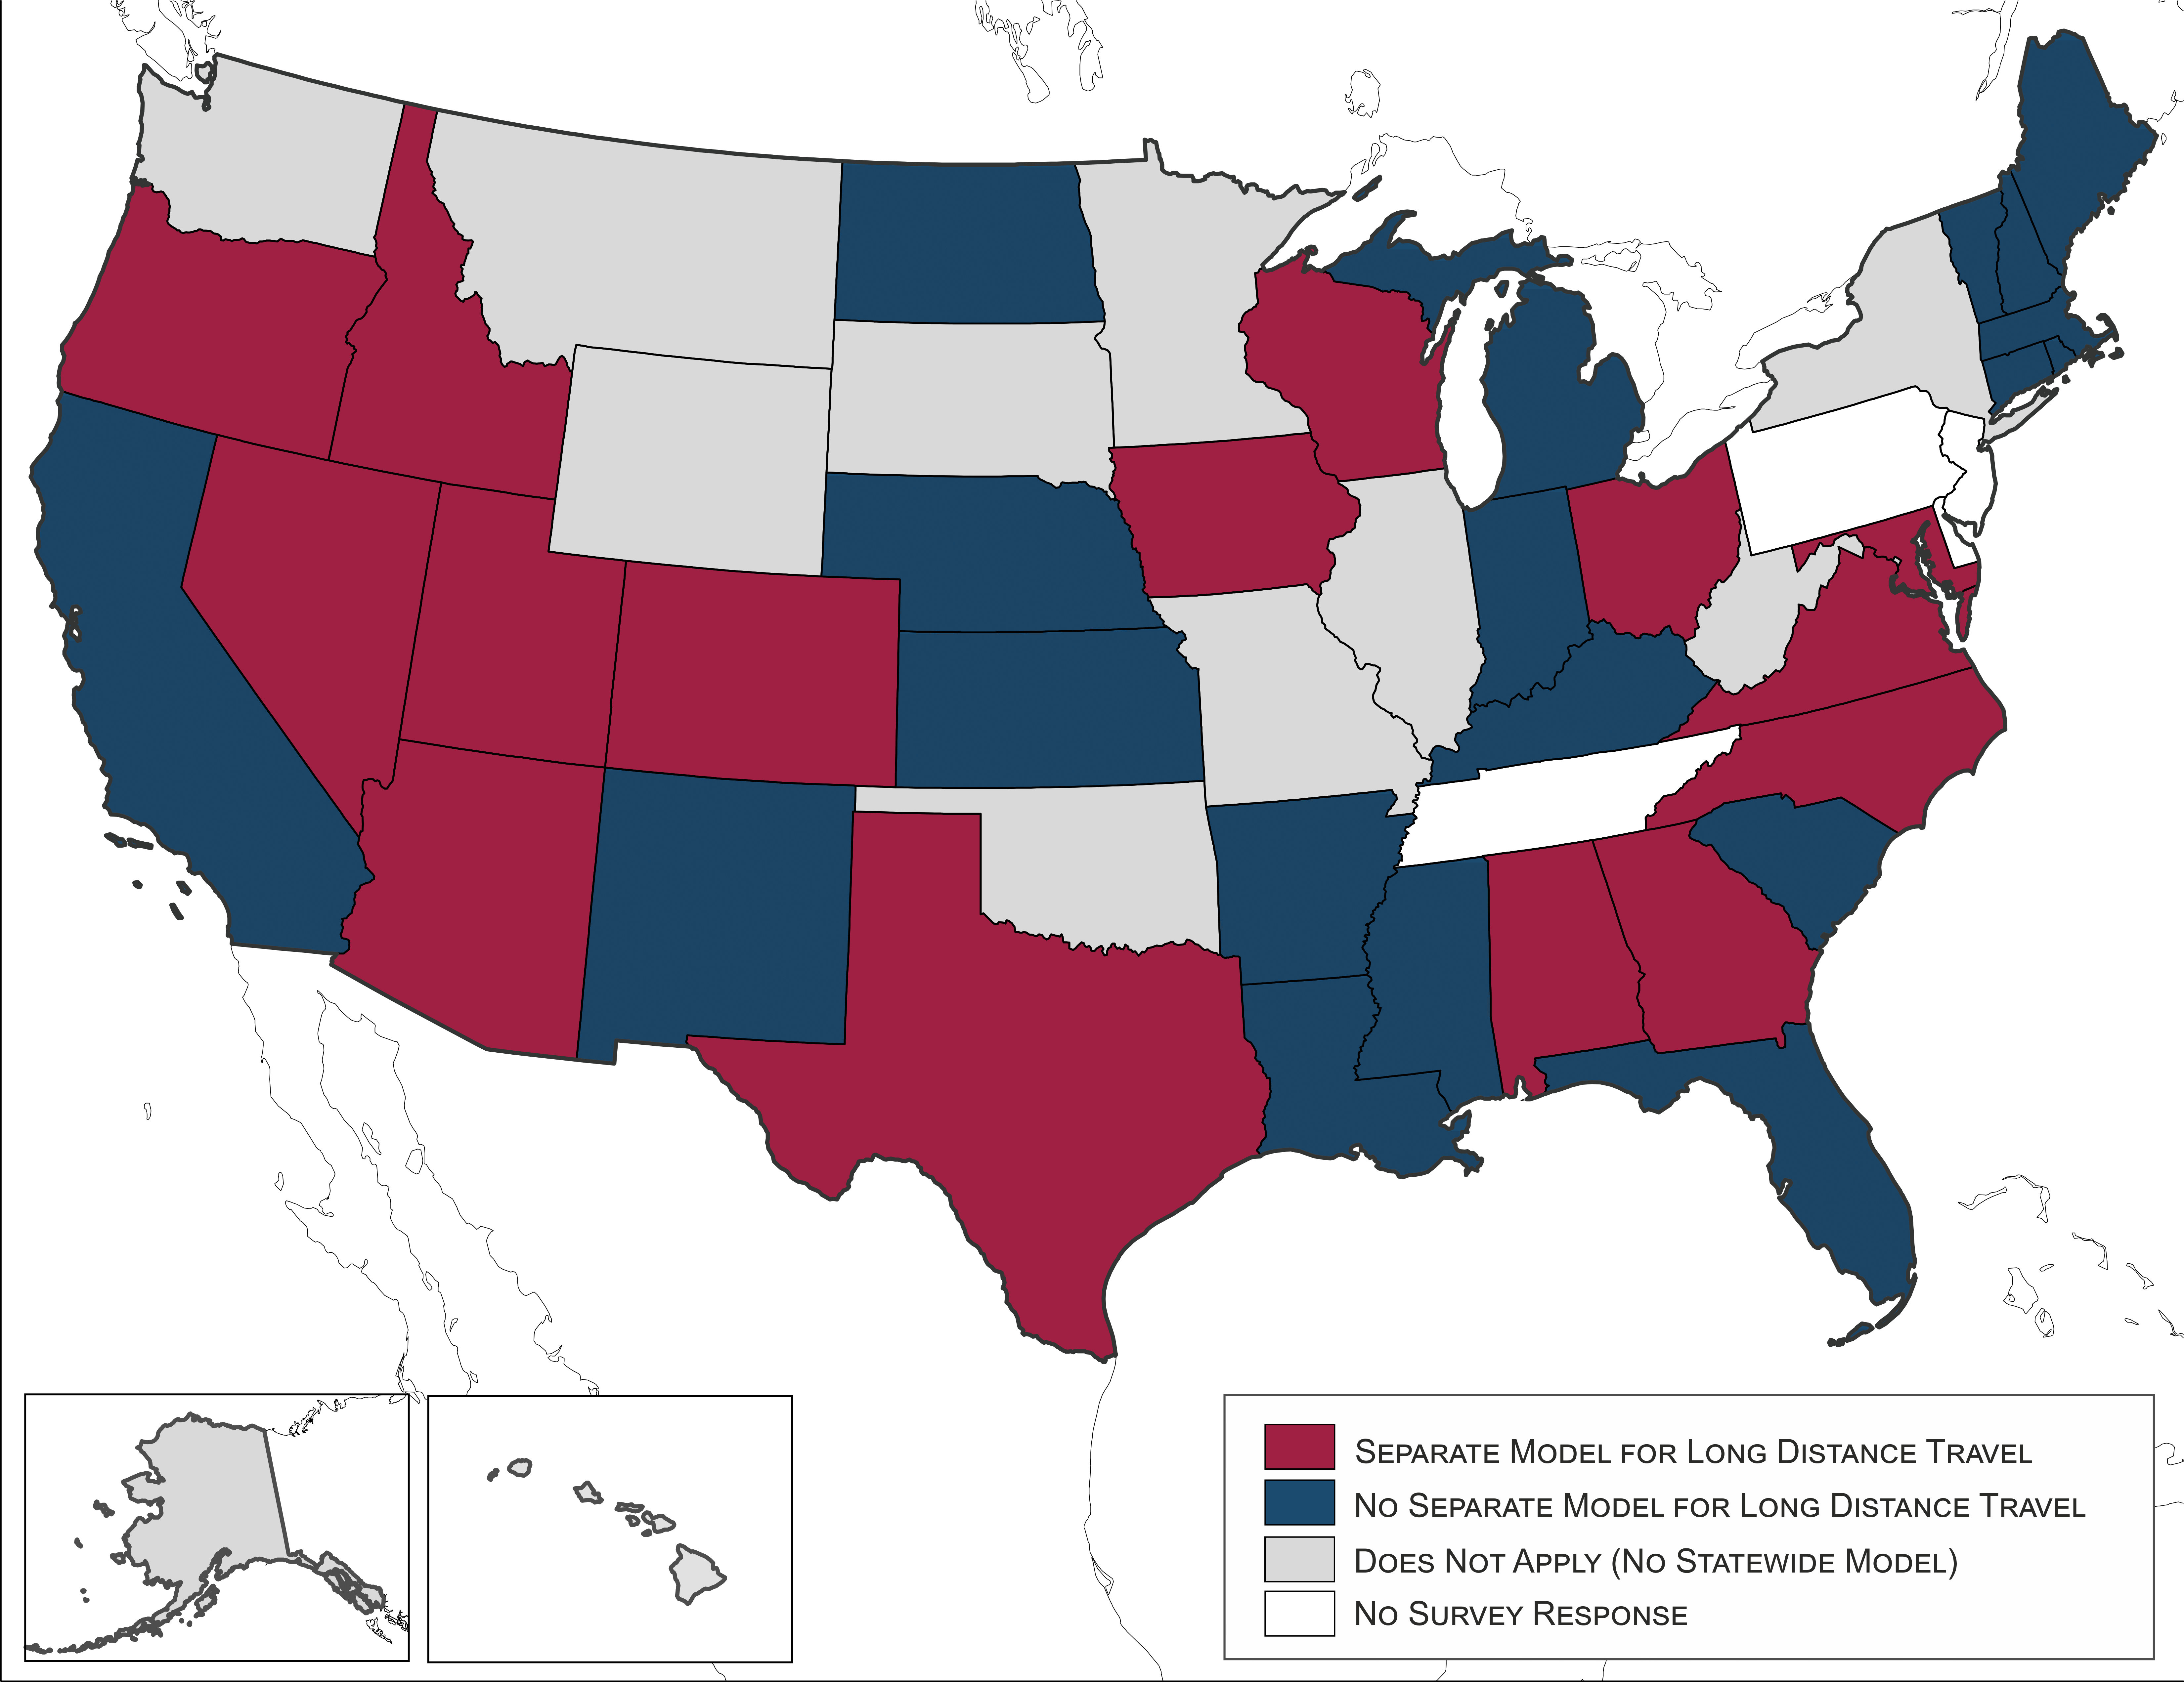
\includegraphics[width=6.4in]{graphics/17-person-long-distance-states}
\caption{States that operate separate long-distance models for person travel}
\label{fig:person-long-distance-states}
\end{figure}

A wide variety of sources are used for trip generation of long-distance trips, as summarized in Figure \ref{fig:person-long-distance-generation}. Iowa is currently the only state that uses FHWA's national long-distance person model \citep{outwater14, outwater15} and trip rates provided in NCHRP Report 735 \citep{schiffer12}. Arizona, Maryland, and North Carolina use the long-distance model NELDT \citep{moeckel11}, which is based on trip frequencies reported in the long-distance element of the 2001 NHTS.

\begin{figure}   % 18
\centering
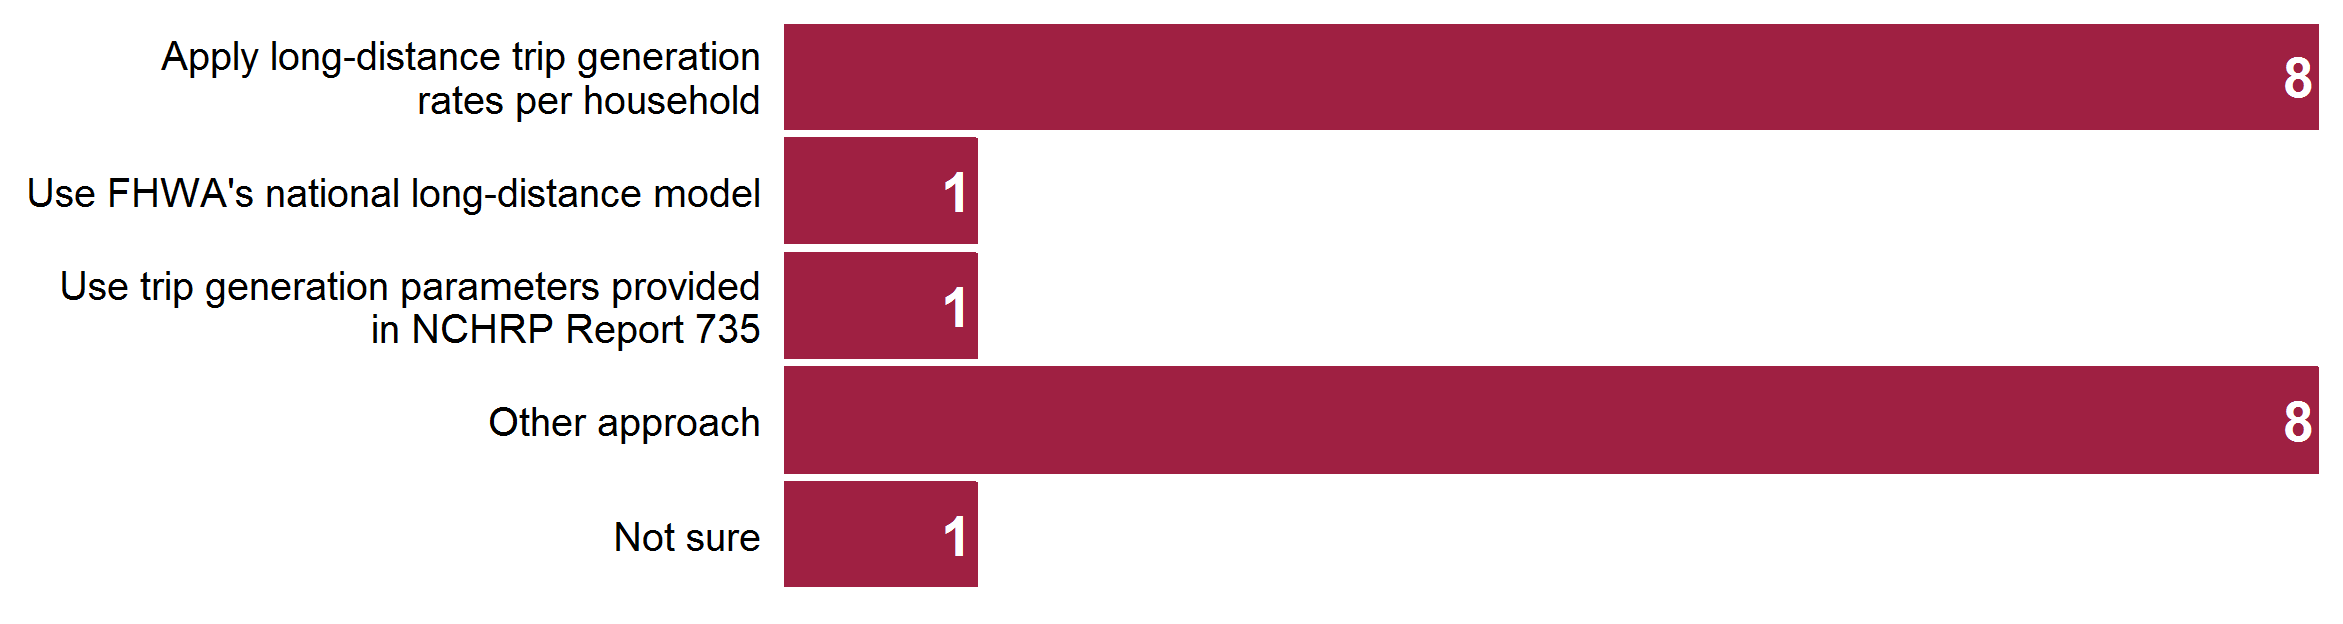
\includegraphics[width=6.4in]{graphics/18-person-long-distance-generation}
\caption[Travel demand generation rates for person long-distance travel]{Travel demand generation rates for person long-distance travel (multiple answers allowed)}
\label{fig:person-long-distance-generation}
\end{figure}

Most long-distance models use traditional gravity models for trip distribution, as shown in Figure \ref{fig:person-long-distance-distribution}. The shortcomings of this approach have already been discussed in \S\ref{sec:person-demand-modeling}, though using separate gravity models for short- and long-distance travel makes that criticism less severe. Five states use advanced logit-based destination choice models, making the one-third share of this approach similar to the pattern found for short-distance travel models.

\begin{figure}   % 19
\centering
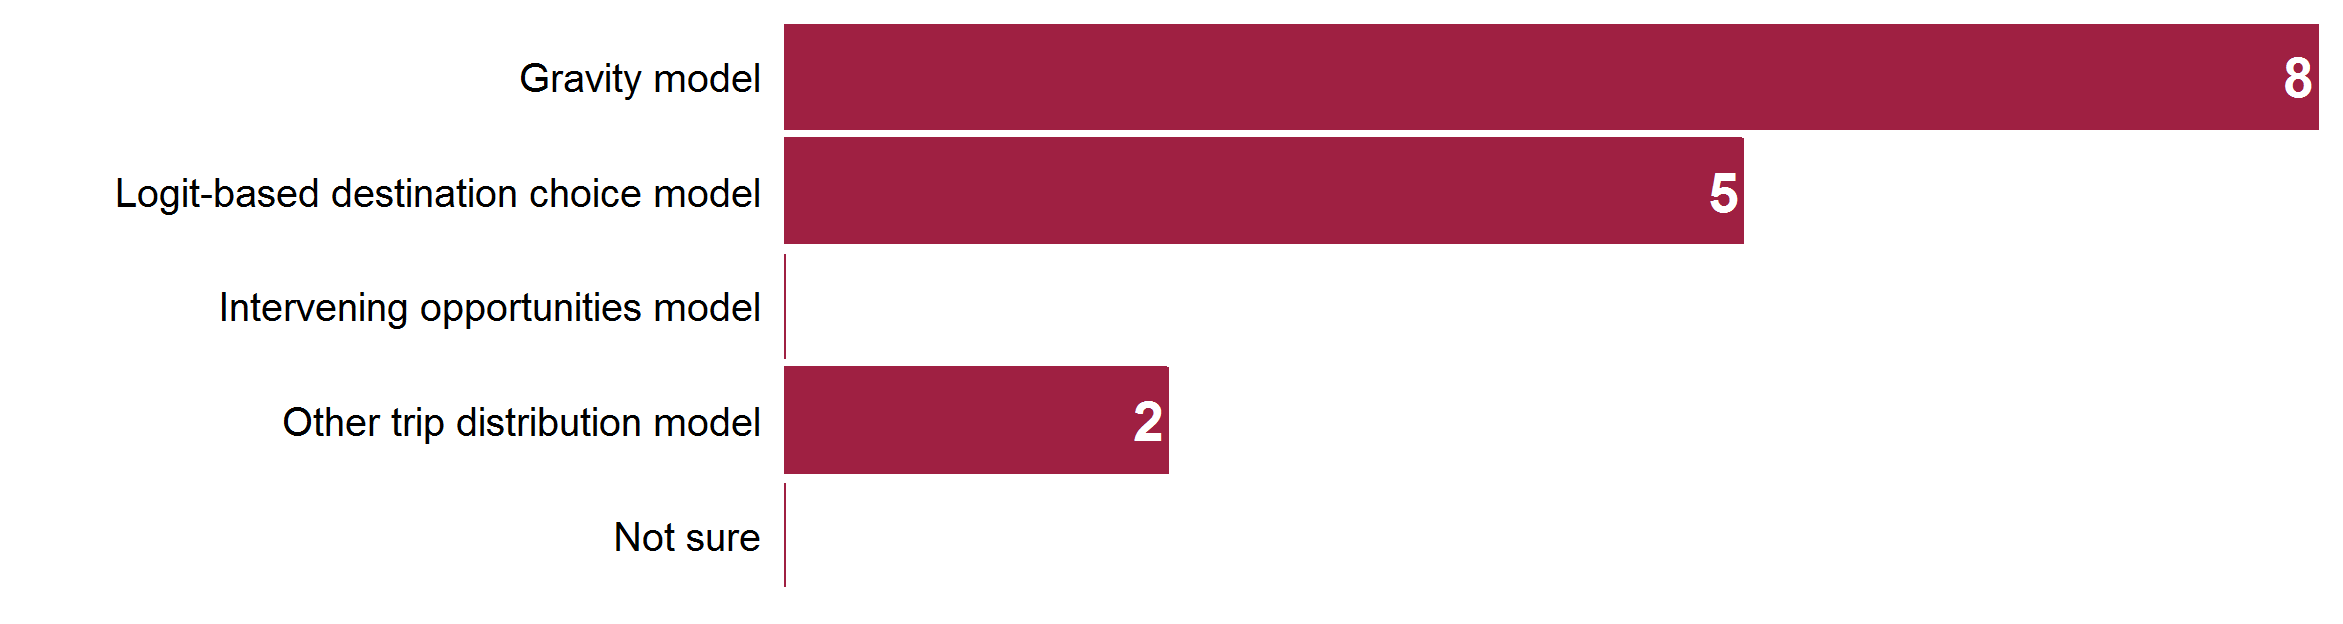
\includegraphics[width=6.4in]{graphics/19-person-long-distance-distribution}
\caption{Frequency of trip distribution models for long-distance person travel}
\label{fig:person-long-distance-distribution}
\end{figure}

About half of all long-distance models apply nested multinomial mode choice models (Figure \ref{fig:person-long-distance-mode-choice}). Wisconsin uses a multinomial model, and Utah applies static mode shares (consistent with their short-distance mode choice model). Colorado selected other mode choice model, as all intra-state trips are handled by the short-distance mode choice model; no mode choice model is planned at this time for interstate trips. Alabama, Arizona, Maryland and Nevada generate long-distance trips for autos only.

\begin{figure}   % 20
\centering
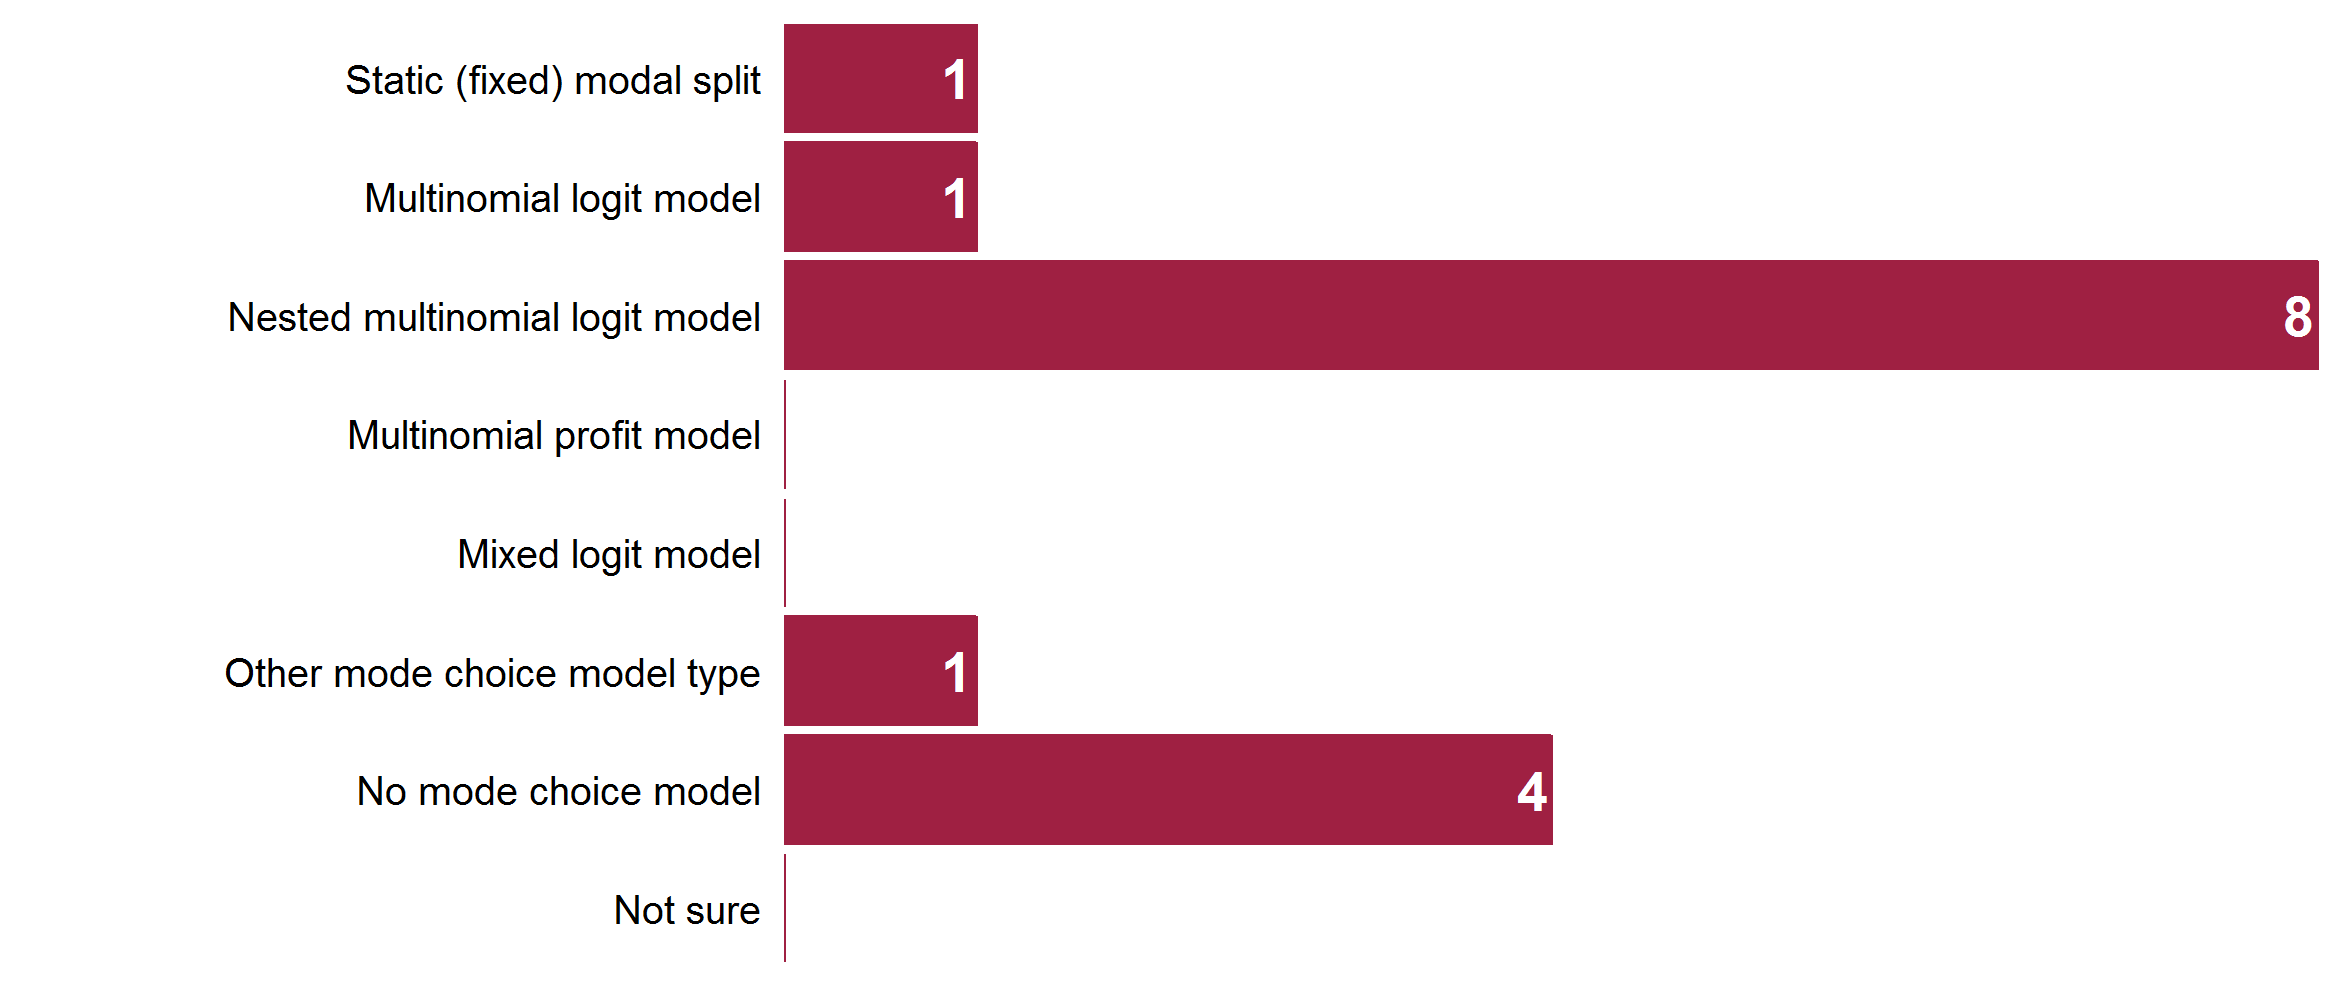
\includegraphics[width=6.4in]{graphics/20-person-long-distance-mode-choice}
\caption{Frequency of mode choice models for long-distance travel}
\label{fig:person-long-distance-mode-choice}
\end{figure}

The modes of transportation represented by long-distance travel models are shown in Figure \ref{fig:person-long-distance-modes}. Obviously, non-motorized travel is not modeled for long-distance travel. All states model the auto mode, and five models distinguish drive-alone from shared-ride. Many include bus, rail, and air, with Georgia, Maryland, Oregon and Texas offering the option to represent high-speed rail explicitly. California has developed a separate high-speed rail model that is not integrated with the statewide model, as described in \S\ref{sec:california-hsr-model} (page \pageref{sec:california-hsr-model}).

\begin{figure}   % 21
\centering
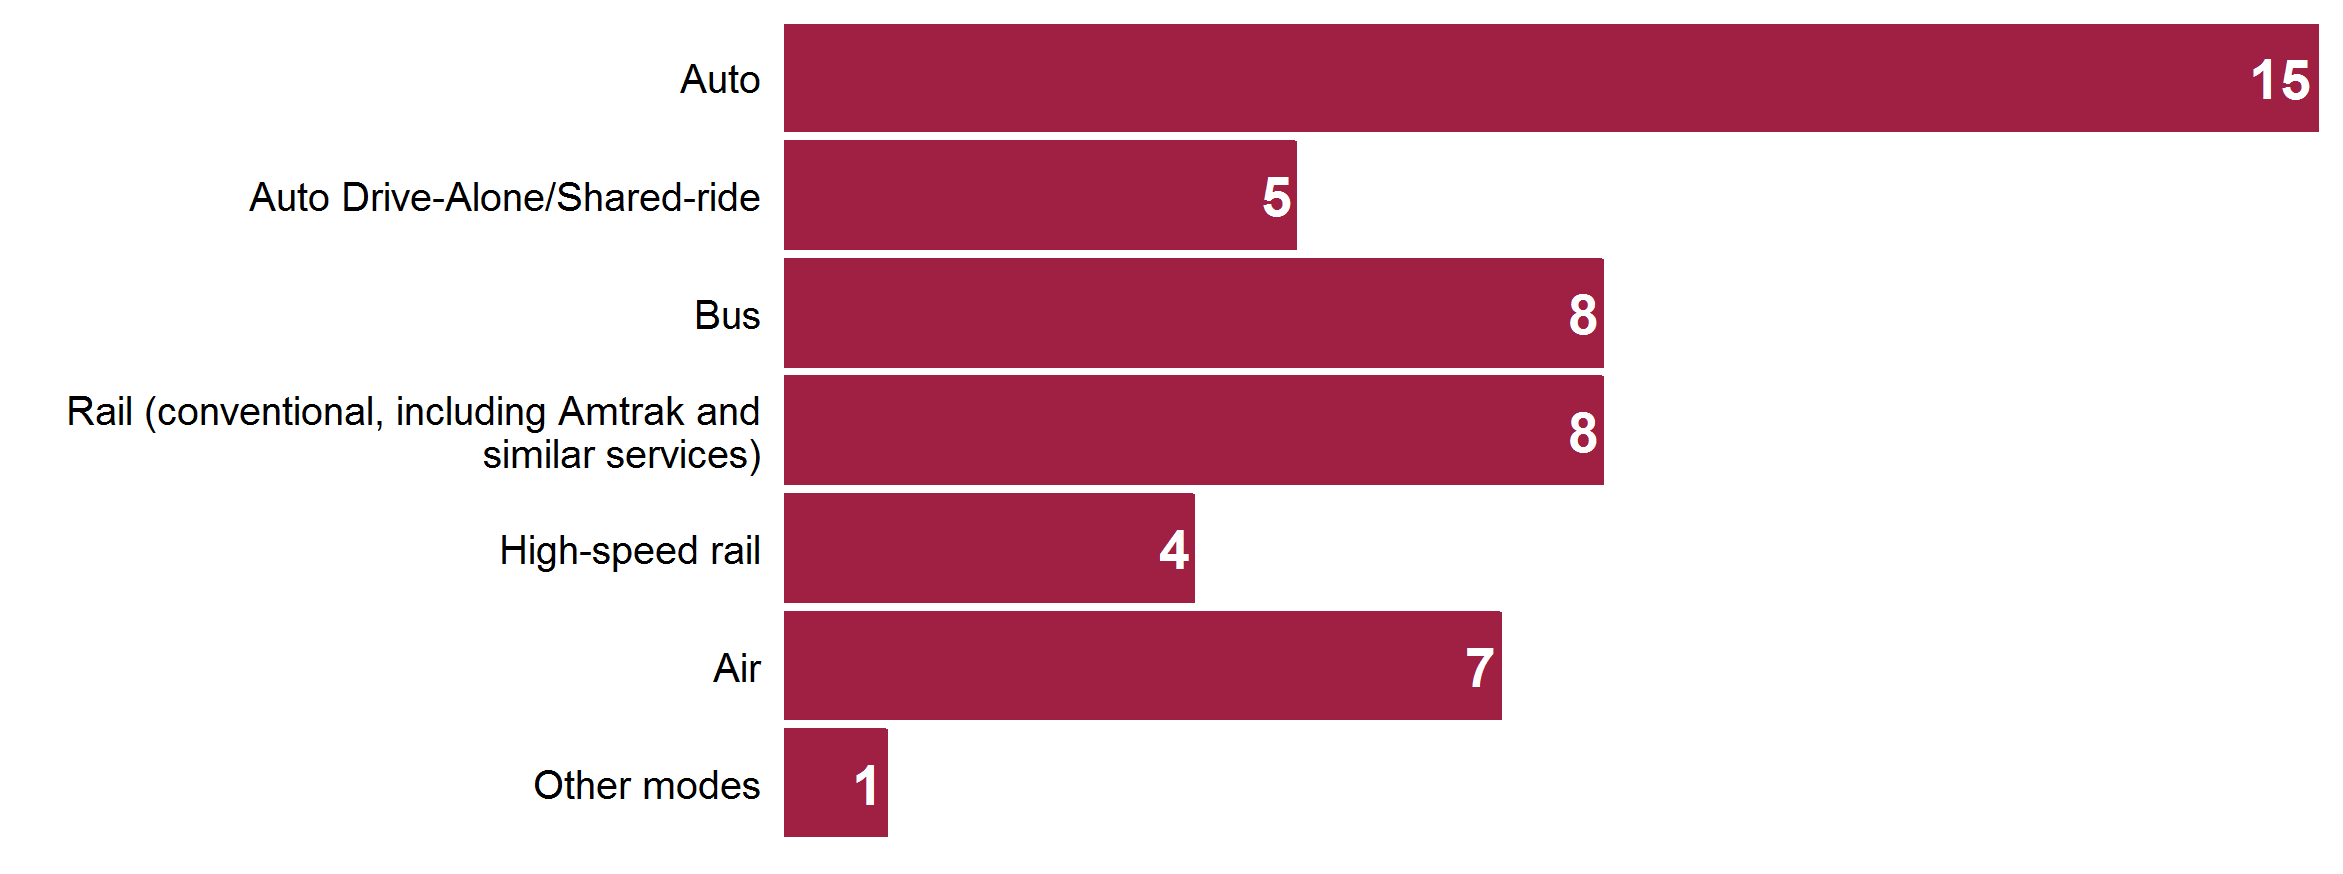
\includegraphics[width=6.4in]{graphics/21-person-long-distance-modes}
\caption[Modes represented in long-distance person mode choice models]{Modes represented in long-distance person mode choice models (multiple answers allowed)}
\label{fig:person-long-distance-modes}
\end{figure}

\section{ Freight models}

Travel demand modeling has traditionally focused on person travel by auto. This is not surprising, as autos generate over 90 percent of all vehicle-miles traveled \citep{fhwa16b}, while trucks make up only 4.1 percent of all registered vehicles and only 2.5 percent of all new vehicle sales in the United States \citep{bea16}. However, trucks generate the core demand for transportation infrastructure maintenance. For example, the rear axles of a typical 13-ton van cause 1,000-times the structural damage of a car (\cite{small89}:11). Ketcham estimated that 95 percent of all highway damage is caused by heavy trucks (\cite{mackenzie92}:9). Trucks also consume 25 percent of all fuel in the United States \citep{bts16}, contributing disproportionately to greenhouse gas emissions. Furthermore, growth in freight transportation is expected to significantly outpace growth in passenger transportation (\cite{chow10}:1012). Moreover, easing freight travel has become a mantra for economic development \citep{mckinnon06}. The ratio between freight-miles traveled and the Gross Domestic Product, also known as the freight-transportation intensity, shows a strong (yet gradually declining) relationship between freight activity and economic growth.

Given their disproportional impact upon the transportation system, it is not surprising that most statewide models account for freight modeling (Figure \ref{fig:freight-models-frequency}), particularly in areas with high levels of congestion. As freight tends to make up a higher share of traffic on rural roads, statewide models tend to have a larger share of freight traffic than urban models. Therefore, statewide models tend to pay more attention to freight flows, often distinguishing short- and long-distance freight flows. While short-distance trucks are covered by 21 states (62 percent of all states with statewide models), long-distance trucks are modeled by 26 states (76 percent). Connecticut uses static truck trips tables, and Nebraska plans to add them within the next year. Doing so enables these states to at least account for truck volumes on the network, even though truck flows would not be scenario sensitive.

\begin{figure}   % 22
\centering
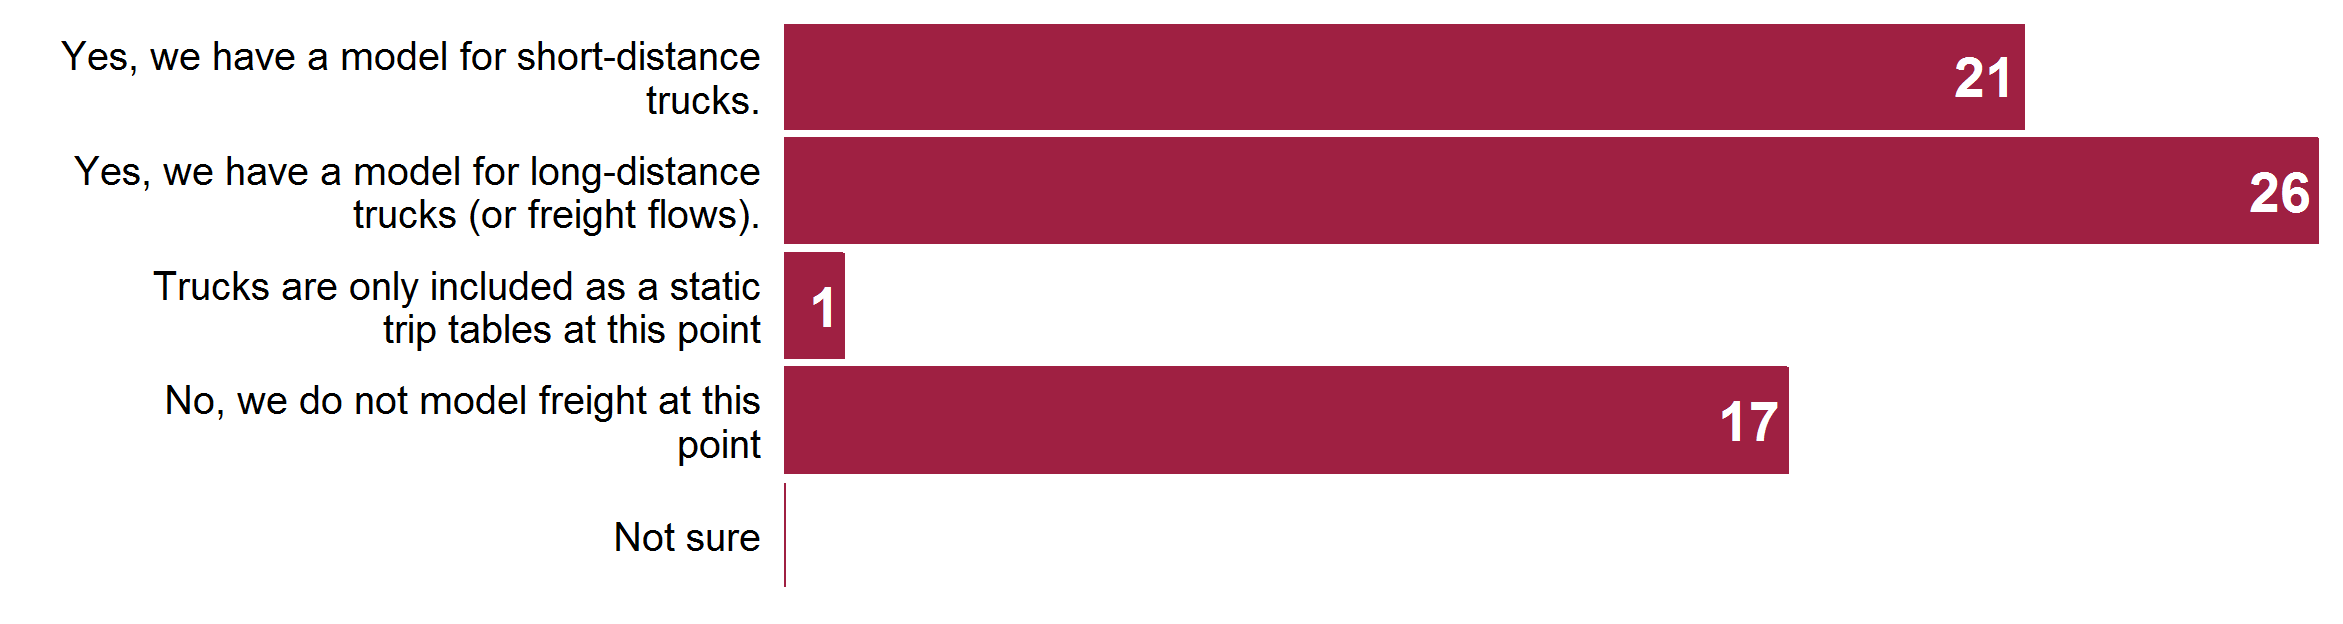
\includegraphics[width=6.4in]{graphics/22-freight-models-frequency}
\caption{Frequency of freight models in statewide models}
\label{fig:freight-models-frequency}
\end{figure}

Of the 21 states that model short-distance trucks, 19 use trip-based models, and only Ohio and Oregon use tour-based truck models. The limitations of trip-based truck models have been discussed extensively in the literature \citep{holguinveras13}, yet it is no surprise that tour-based models are uncommon in statewide models. The heterogeneous travel behavior of trucks (depending, among other factors, on truck type and commodities carried) and the limited freight data availability (much more so than for auto travel) make it inherently challenging to represent tour-based travel behavior for trucks. However, a few operational tour-based models in addition to Ohio and Oregon have been implemented for Alberta \citep{hunt07}, Guatemala City \citep{holguinveras03}, Rome \citep{nuzzolo13} and the San Pedro Bay Ports in Southern California \citep{you12}. Given the increasing interest in freight in many states, it is expected that more will follow the examples of Ohio and Oregon in tour-based truck modeling in the future.

The spatial distribution of long-distance freight models is shown in Figure \ref{fig:freight-long-distance-states}. Clusters of them are apparent in the Southwest, the South, and the Great Lakes area. Freight modeling appears to be less common in states in the northern parts of the U.S. The Interstate 10 corridor and possibly the I-65 corridor (though Tennessee did not participate in this survey) are the only ones that are covered completely by statewide truck models. Several states in the Midwest and New England have not tackled freight flow models yet. Given the especially large volumes of long-distance truck flows on east-west highway corridors, many states might benefit from explicitly modeling them.

\begin{figure}   % 23
\centering
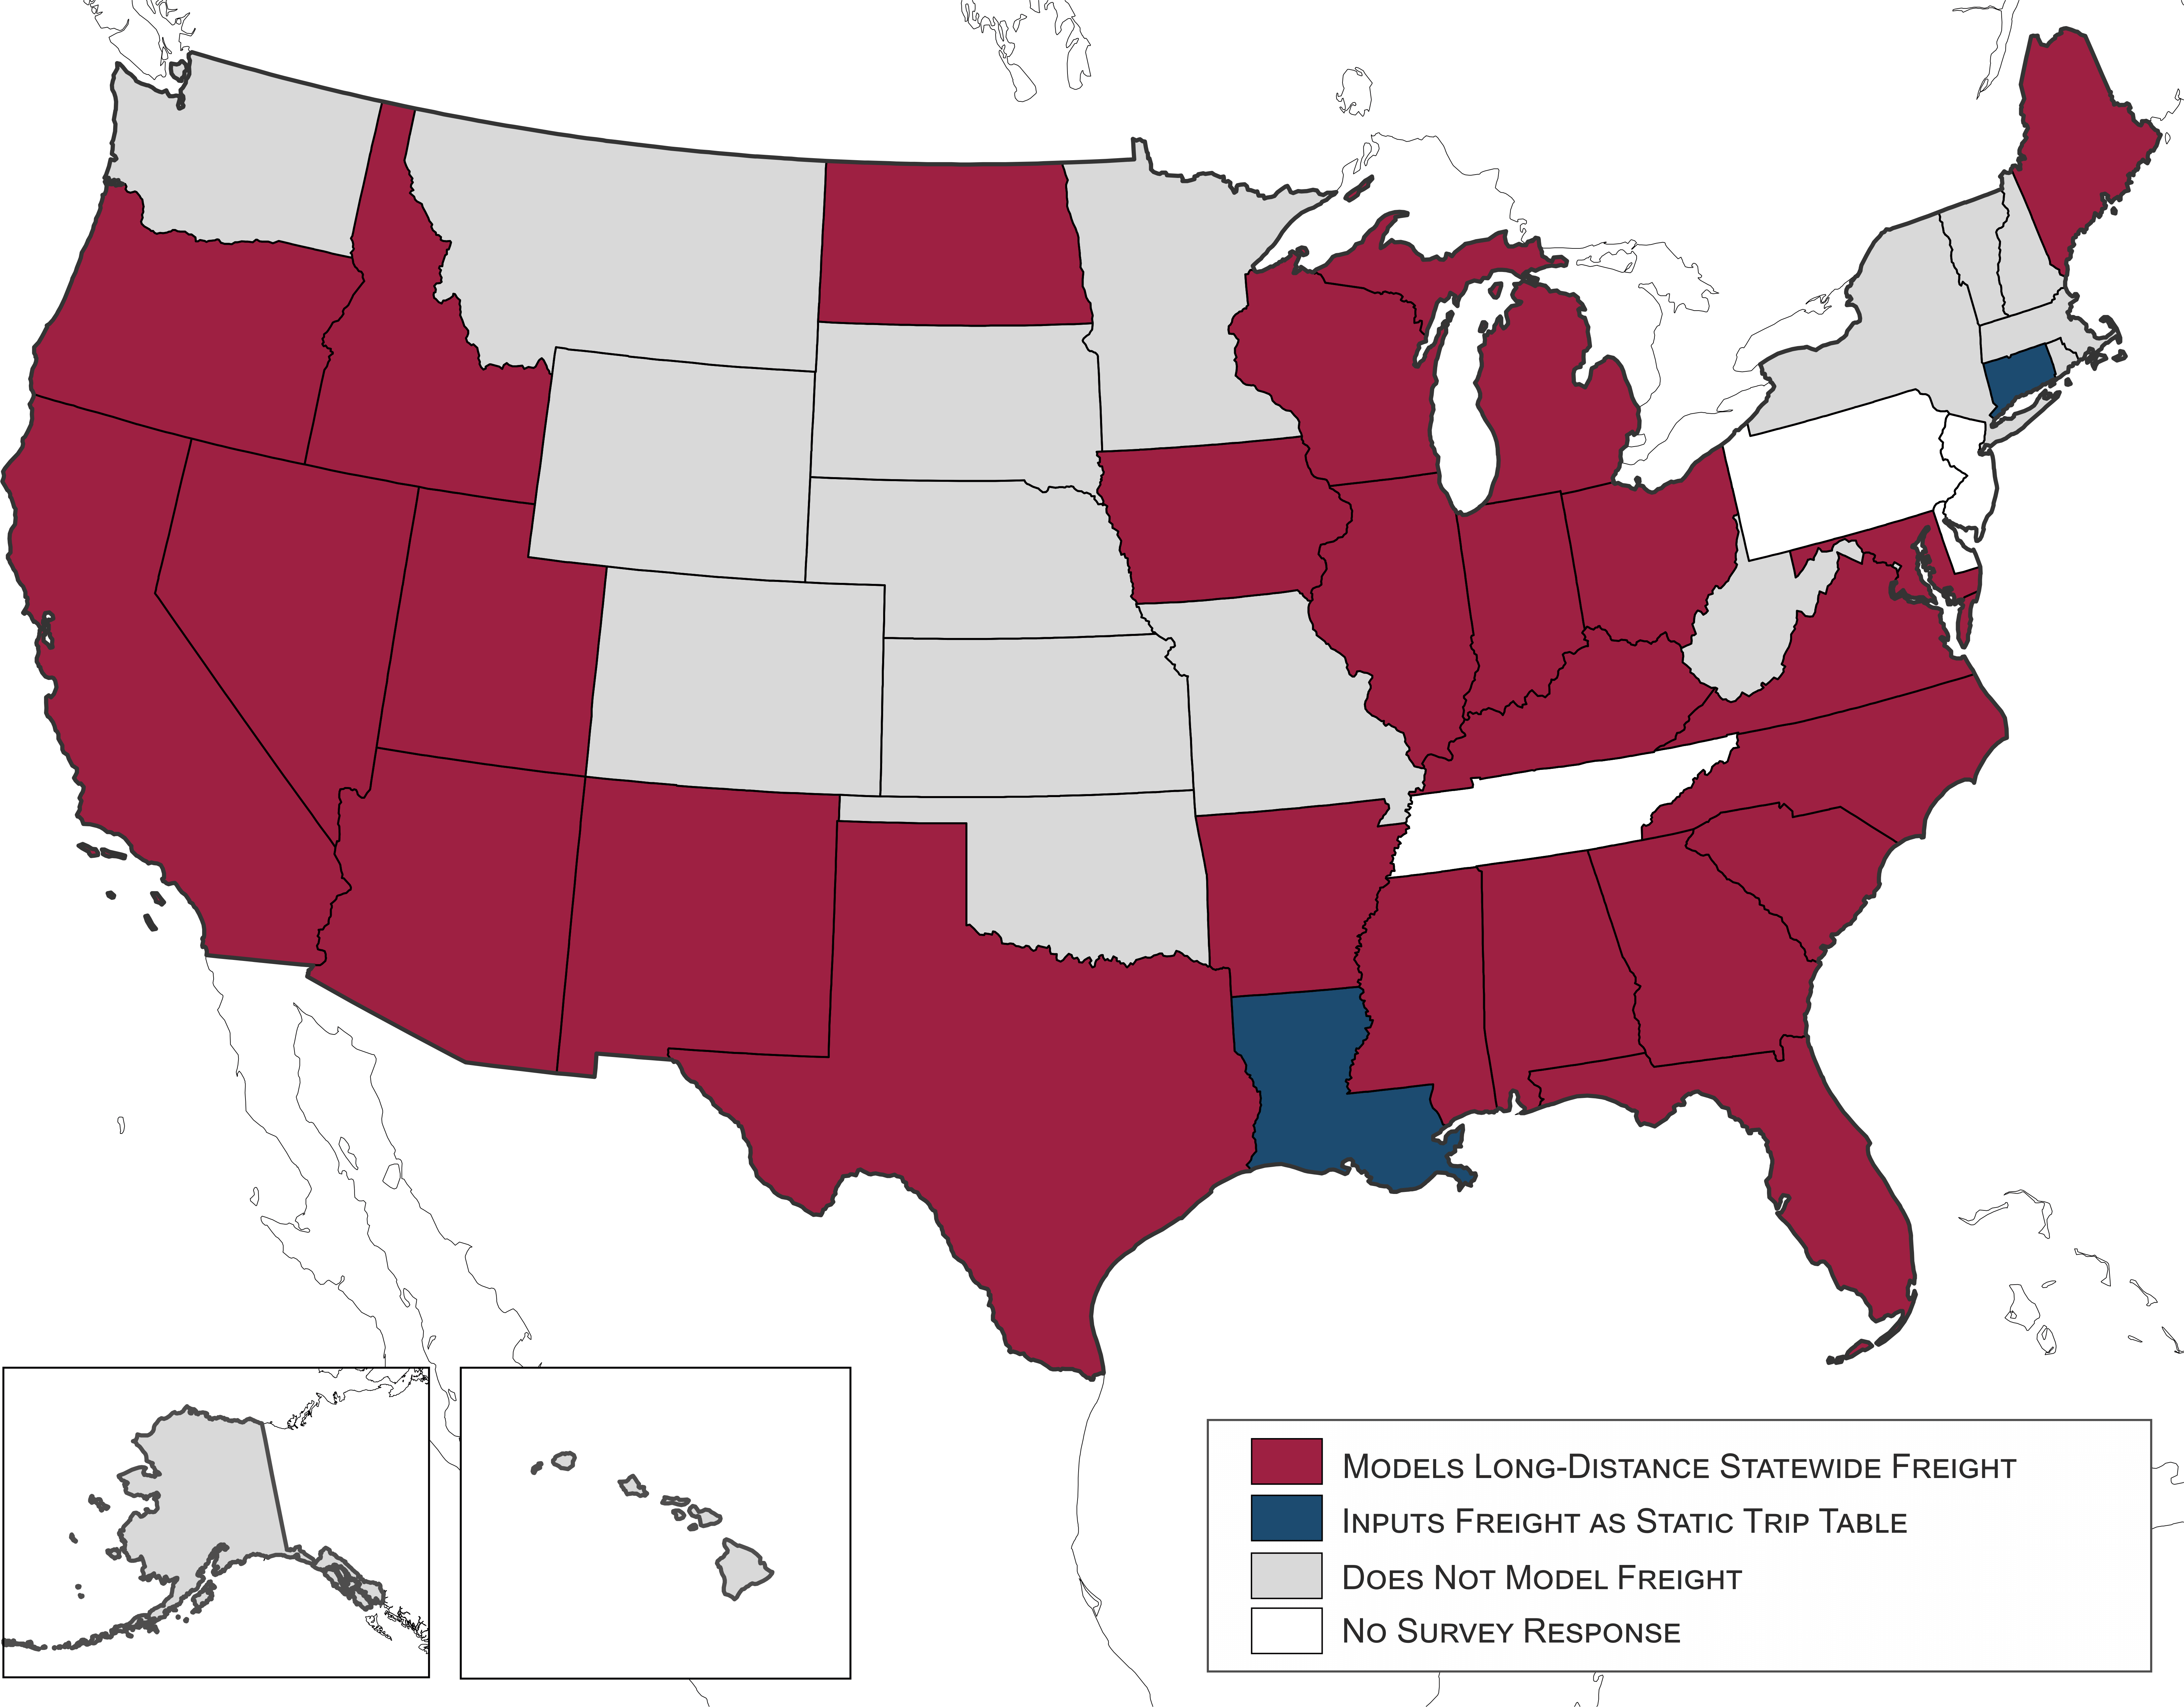
\includegraphics[width=6.5in]{graphics/23-freight-long-distance-states}
\caption{States operating long-distance freight models}
\label{fig:freight-long-distance-states}
\end{figure}

Long-distance truck modeling is dominated by commodity flow models (Figure \ref{fig:freight-long-distance-methods}). Illinois uses a supply chain model, though publicly available data for such modeling approach is very limited. Most of the respondents who reported using commodity flow models in the survey reported that they are based, at least in part, upon origin-destination freight flow data from the Freight Analysis Framework (FAF), as described in \S\ref{sec:traditional-freight-data} (page \pageref{sec:traditional-freight-data}). Presumably, many of these models are not policy-sensitive commodity flow models, but rather static transformations of exogenous FAF commodity flows converted into truck flows. Nine states use FAF payload factors to convert freight flows in tons into truckload equivalents.

\begin{figure}   % 24
\centering
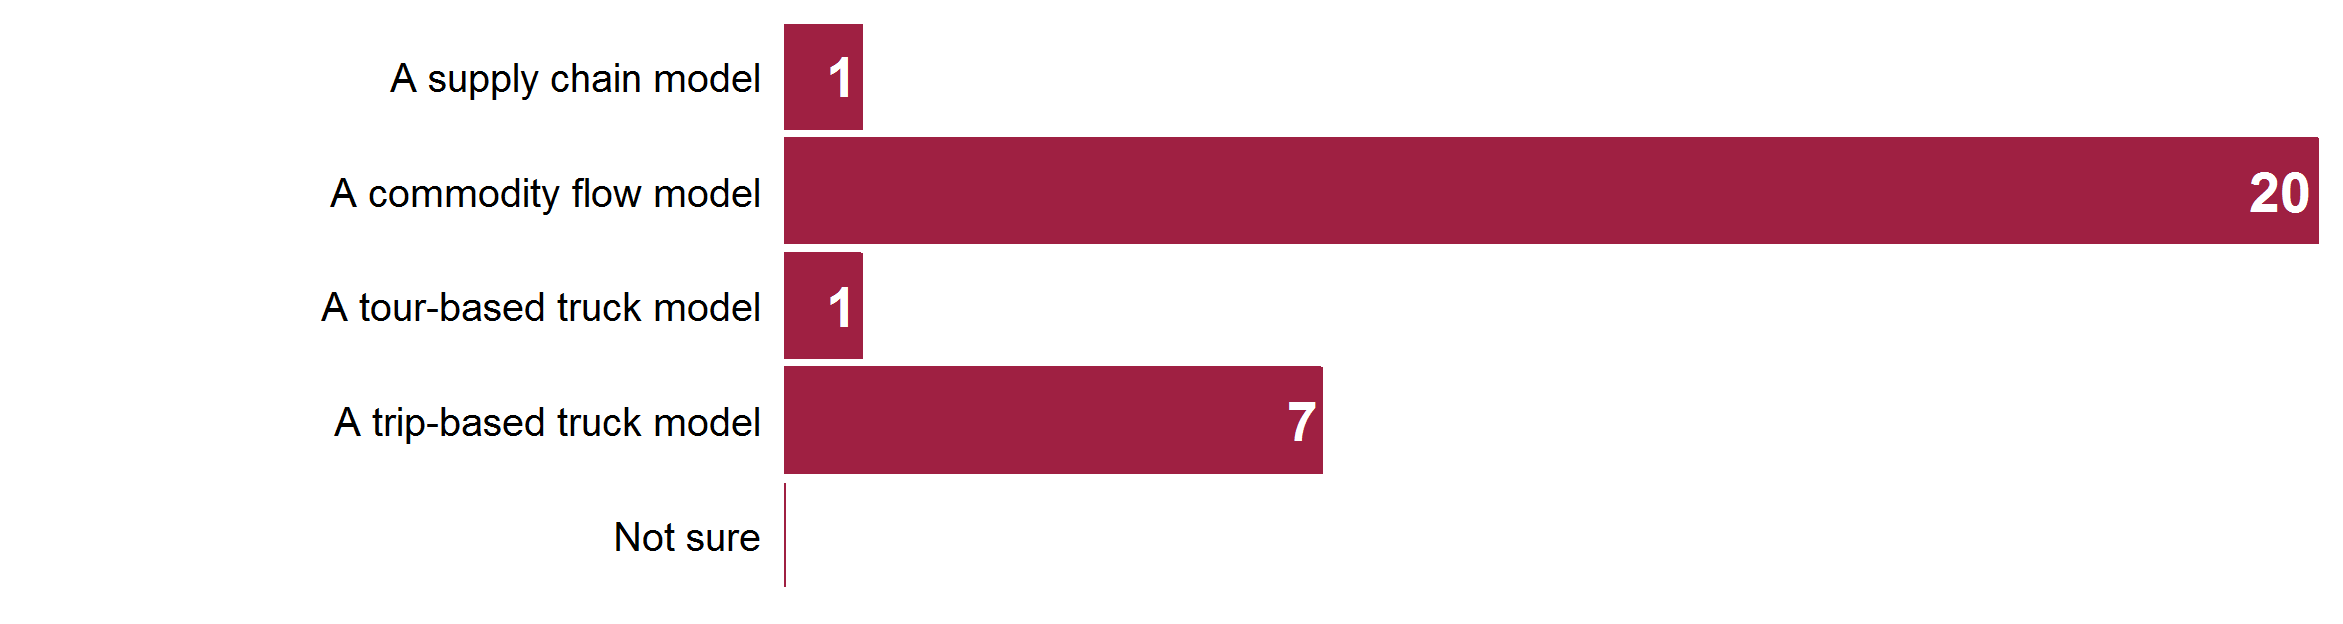
\includegraphics[width=6.4in]{graphics/24-freight-long-distance-methods}
\caption[Frequency of long-distance freight modeling methods]{Frequency of long-distance freight modeling methods (multiple answers allowed)}
\label{fig:freight-long-distance-methods}
\end{figure}

A growing number of states apply mode choice models to freight flows as well (Figure \ref{fig:freight-mode-choice}). Out of 26 states that model long-distance freight flows, six states (23 percent) apply rule-based freight mode choice models. Such models do not attempt to econometrically estimate mode shares, but rather apply simple rules of modal allocation that can be reviewed and changed. For example, rules may include that short-distance flows rarely use rail or water modes, only high-value goods move by air, and vessels can only be used if there is a waterway on at least part of the trip.

\begin{figure}   % 25
\centering
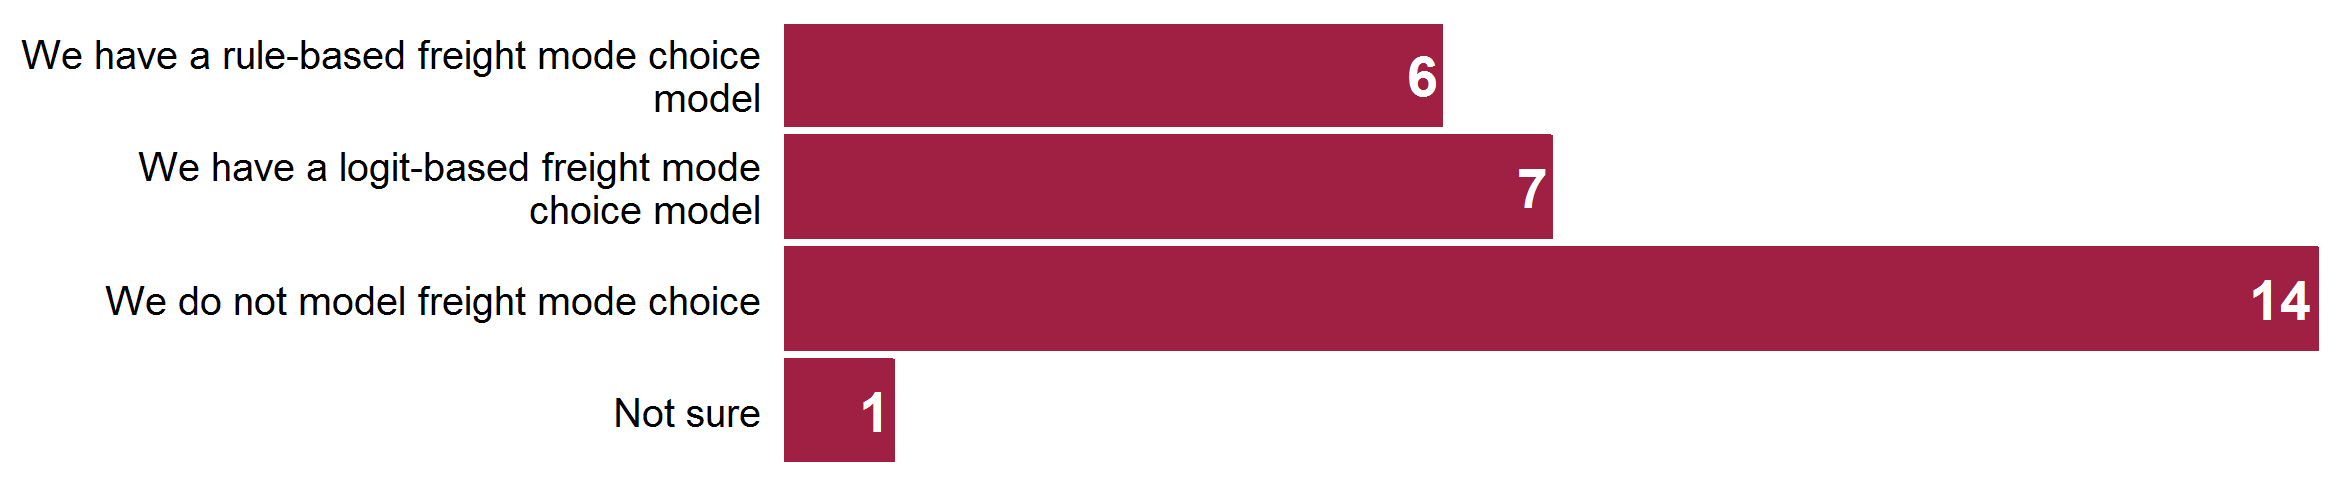
\includegraphics[width=6.4in]{graphics/25-freight-mode-choice}
\caption[Frequency of freight mode choice models]{Frequency of freight mode choice models (multiple answers allowed)}
\label{fig:freight-mode-choice}
\end{figure}

Logit-based freight mode choice models were implemented by Florida, Georgia, Illinois, Ohio, Oregon, Texas, and Virginia. While such models provide rich information on driving factors for mode choice, data limitations often make it challenging to reasonably estimate these models. Many of these logit-based models are designed as so-called freight diversion models (i.e., they model the shift from one mode, such as truck, to another mode, such as rail). Starting with the observed mode share and modeling only the potential shift from one mode to another is a powerful way to deal with data limitations in freight modeling while maintaining some freight mode sensitivities to policy scenarios. Ohio and Oregon use a combination of both rule-based and logit-based mode choice models. About half of the 26 states that model freight long-distance flows do not model freight mode choice at all, but instead generate truck flows only.

Of the 11 statewide models that represent freight mode choice, all include truck and rail as modal options (Figure \ref{fig:freight-long-distance-modes}). Water and Air are modeled in eight and seven states, respectively. California, Ohio, Oregon and Utah even model pipelines, a flow that is inherently difficult to represent because it has the least amount of data available. Accordingly, FAF decided to merge the pipeline and unknown modes. One other mode was mentioned by Utah, where truck-rail intermodal represents a separate mode. It was known that this mode is also used in other states, such as Ohio and Texas, although they did not state so because it was not explicitly requested in the survey.

\begin{figure}   % 26
\centering
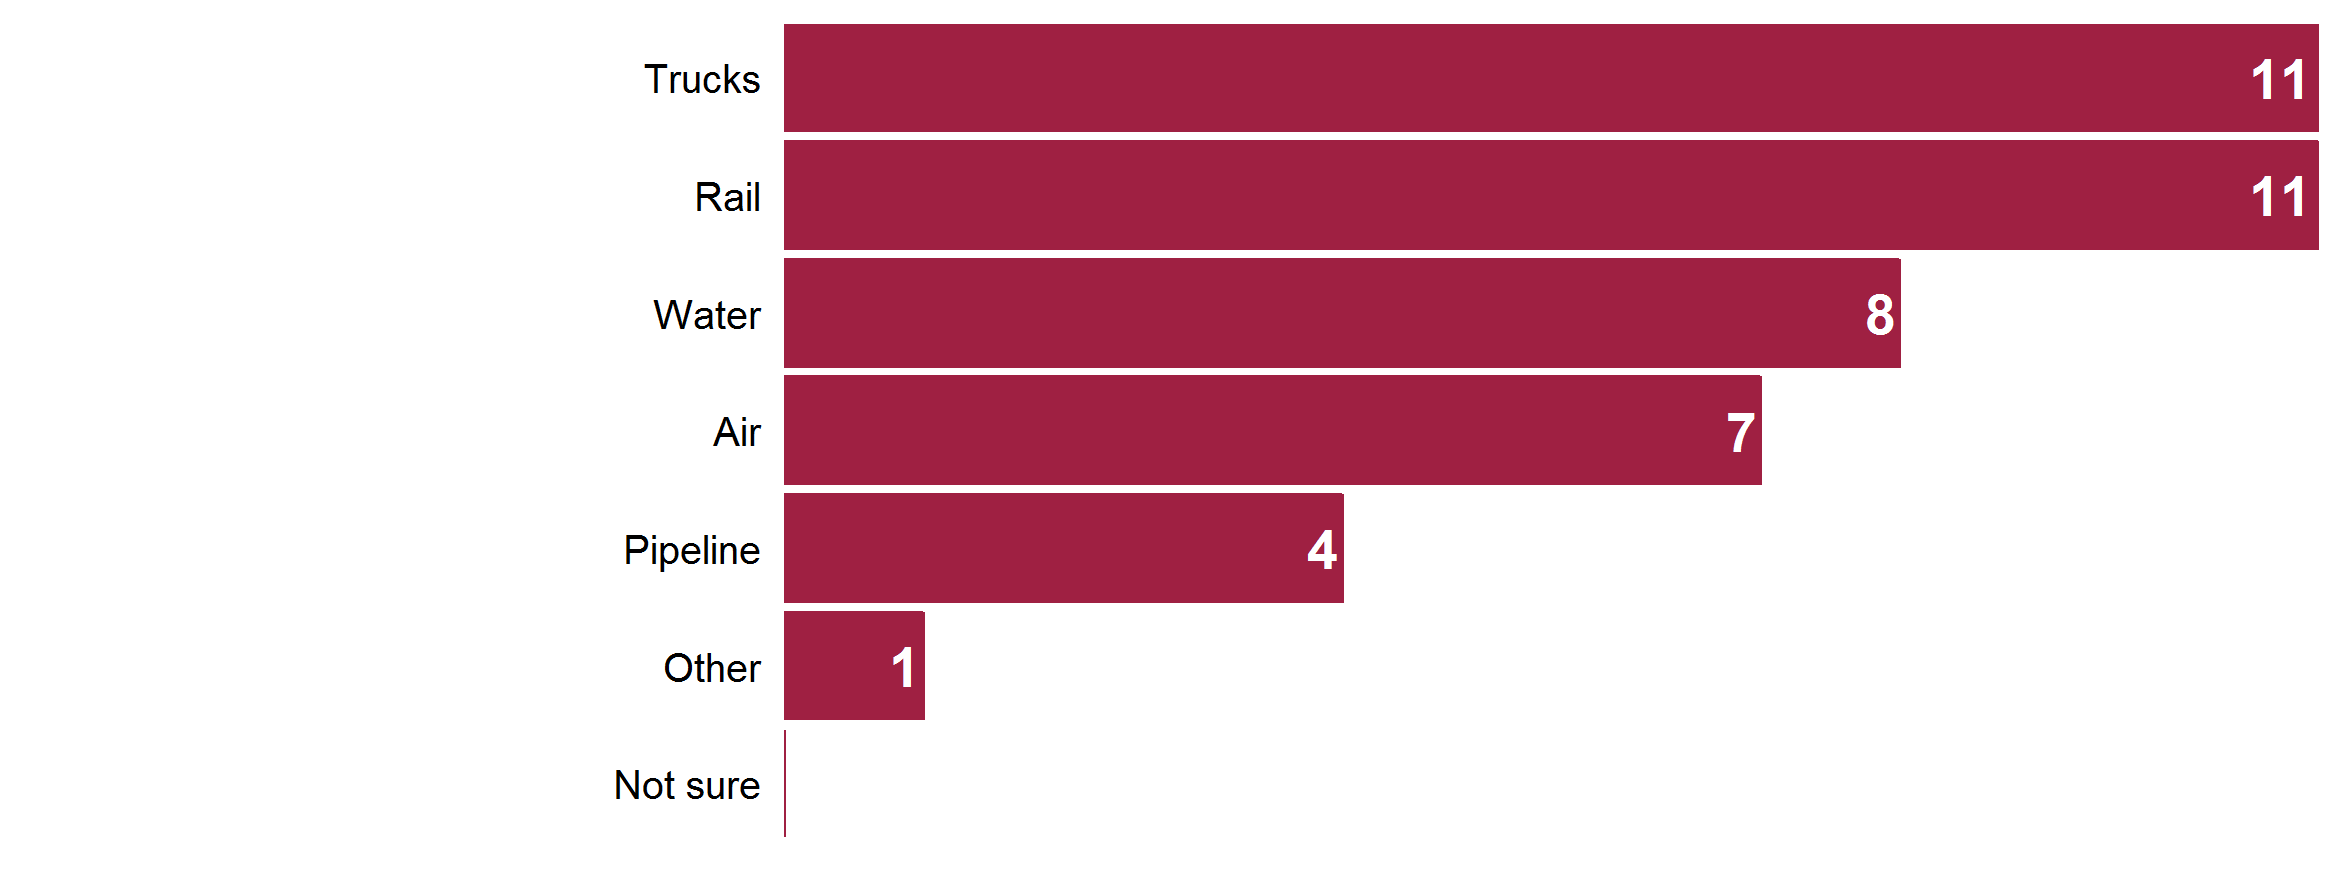
\includegraphics[width=6.4in]{graphics/26-freight-long-distance-modes}
\caption[Modes represented in long-distance freight mode choice models]{Modes represented in long-distance freight mode choice models (multiple answers allowed)}
\label{fig:freight-long-distance-modes}
\end{figure}

\section{Economic models}

Traditionally, statewide transportation models worked with static socio-economic input data. Given the large uncertainty of economic forecasts, many states have moved towards integrating their transportation model with economic forecast models. While such models are not capable of reliably forecasting the future, they add the flexibility of providing socio-economic input data for alternative futures. Many states have a forecast they assume to be the most likely forecast. In addition, each scenario is run with a low-growth forecast and a high-growth forecast, which may be, for example, 5--25 percent above or below the expected growth rate. Having various forecasts allows states to capture some of the uncertainty of future growth, and enables them to test if scenarios are viable under alternative growth scenarios.

In addition to growth rate adjustments, most economic forecast models also represent the interdependencies between various industries and population. If the auto industry enjoys continued growth, firms delivering parts to that industry would grow accordingly. If the unemployment rate in an area is growing the population will likely grow at a slower pace. Accounting for such interdependencies makes stories behind future scenarios richer and increases consistency, and thereby, credibility.

The frequency of economic forecast models is summarized in Figure \ref{fig:economic-model-frequency}. Externally prepared commercial forecasts are the most frequent source of future socio-economic data, closely followed by forecasts developed by other state agencies. Illinois and New Hampshire do not need or use an economic forecast or model, as they only apply the model in the base year.

\begin{figure}   % 27
\centering
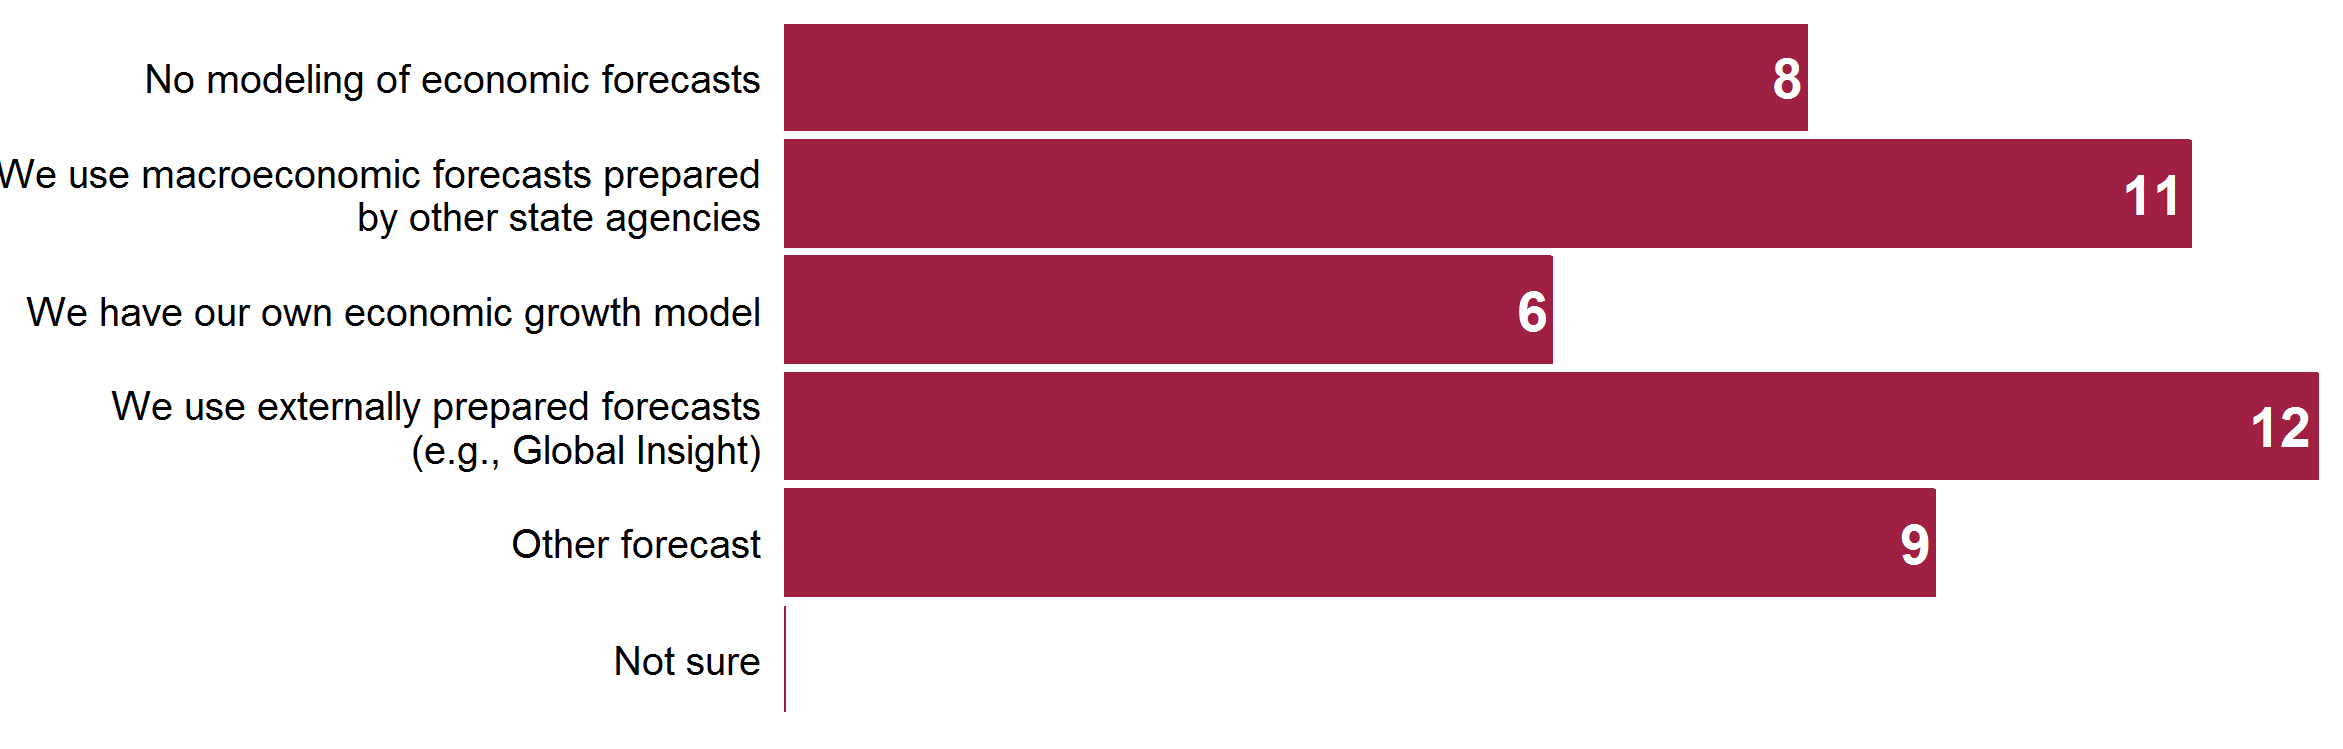
\includegraphics[width=6.4in]{graphics/27-economic-model-frequency}
\caption[Frequency of economic forecast models]{Frequency of economic forecast models (multiple answers allowed)}
\label{fig:economic-model-frequency}
\end{figure}

Respondents in the nine states who selected ``Other forecast'' mentioned that they:
\begin{itemize}
\item Prepare their own forecast,
\item Use the REMI economic forecasting model,
\item Derive population growth forecasts from Longitudinal Employment Household Dynamics (LEHD) and Woods \& Poole population trends, and
\item Work with universities or local consultants to generate forecasts.
\end{itemize}

The agency that operates the transportation model creates their own forecast of socioeconomic data in only six states (or 18 percent of those that have statewide models). This is not to be criticized, as economic forecasts are challenging. However, this likely limits the number of growth rate scenarios that can be run with the transportation model. While a few alternative growth scenarios may be sufficient, agencies that operate their own models may work with a larger number of different growth assumptions.

The distribution of base and future model years are visualized in Figure \ref{fig:base-and-future-years}. Base years cluster around 2010, as expected, while future years dominate in 2015, 2020, 2030, 2035 and particularly in 2040. Beyond that, New York models 2044, California 2050 and Nevada 2060. Several models can provide forecasts for any future year within their model time frame. This is achieved by interpolating between five or 10-year model runs. While this approach assumes a somewhat artificial linear growth between two modeled years, interpolation provides additional data for years the model cannot be run.

\begin{figure}   % 28
\centering
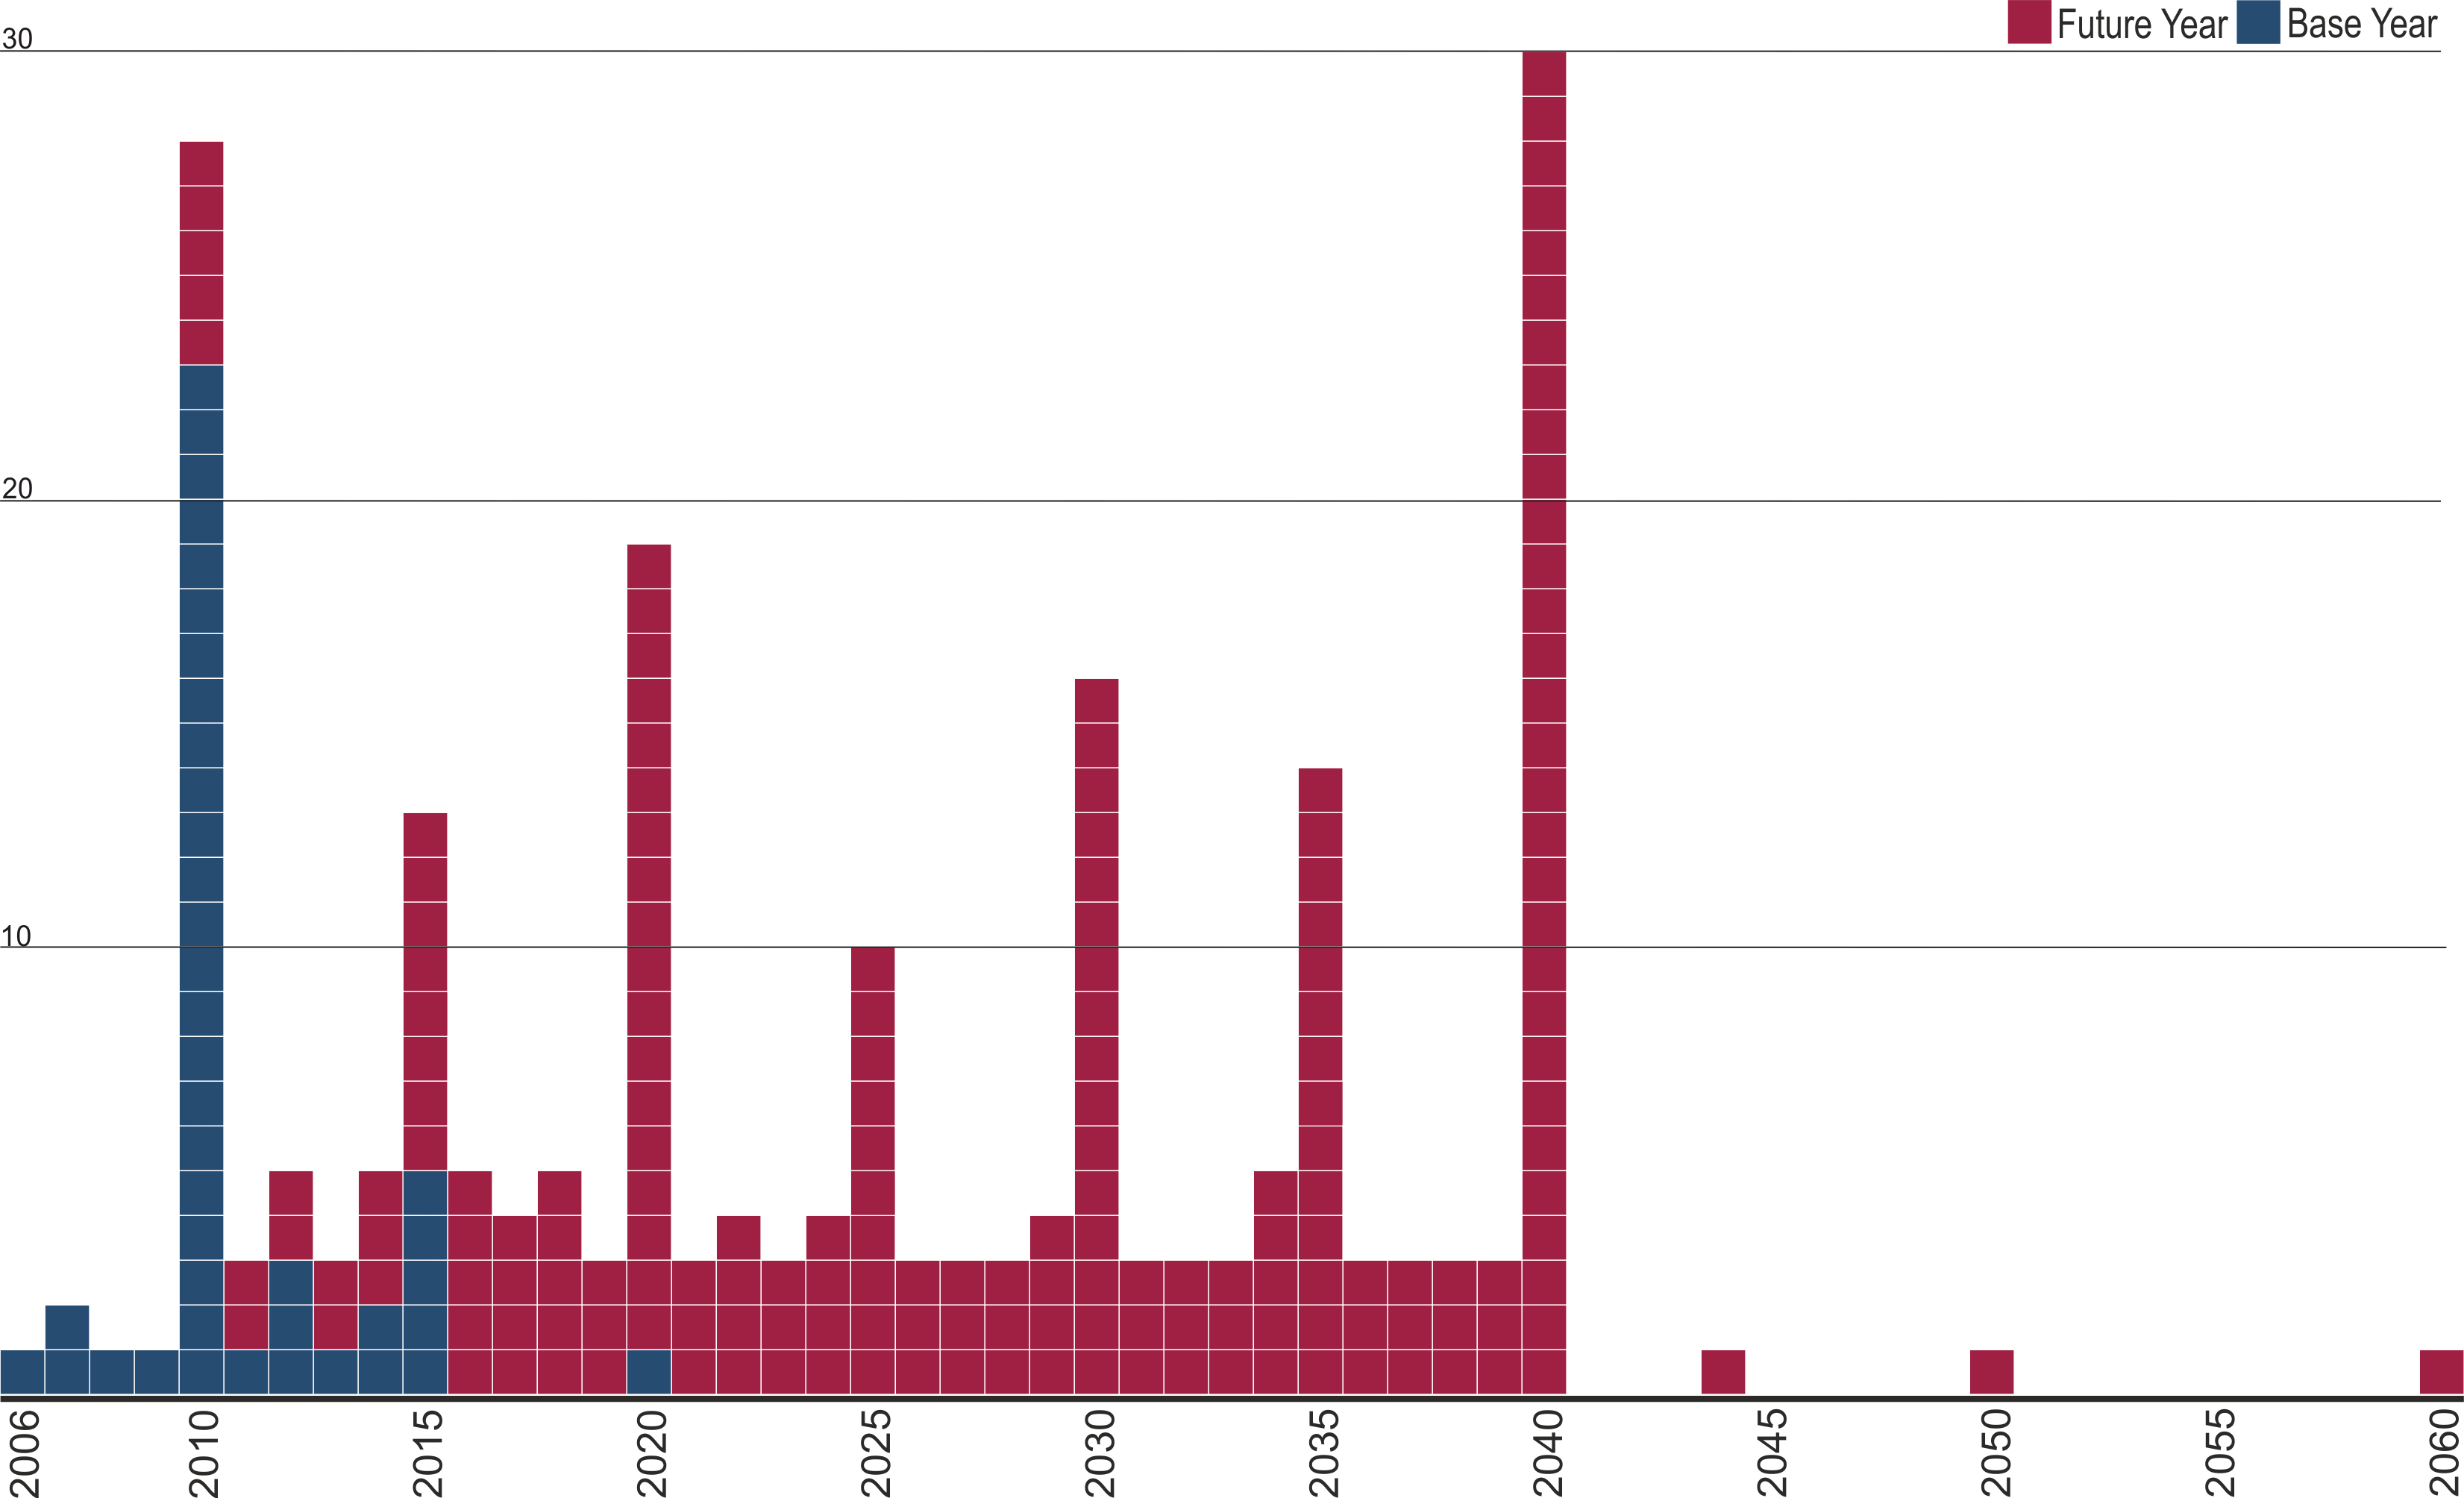
\includegraphics[width=6.4in]{graphics/28-base-and-future-years}
\caption{Distribution of base and future years in statewide models}
\label{fig:base-and-future-years}
\end{figure}

\section{Land use models}

Land use models can be integrated with travel demand models to reflect the interactions between the transportation system and land use development. Both households and businesses prefer locations with higher accessibilities, all else being equal, and are therefore influenced by travel times forecasted using transportation models. The location choices of households, businesses, and developers, in turn, influences the origins and destinations of travel demand calculated in the transportation model. The integration of land use with transportation models has proven to improve model sensitivities in scenario analyses \citep{conder02}. This integration has been visualized schematically in Figure \ref{fig:landuse-transport-feedback}.

\begin{figure}
\centering
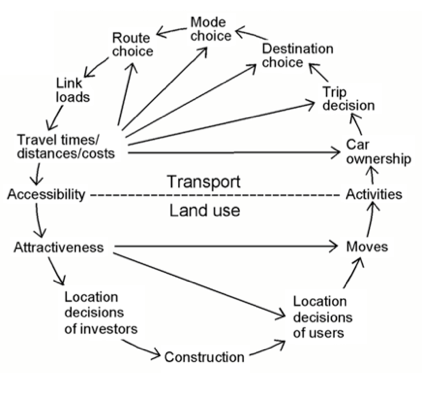
\includegraphics[scale=0.5]{graphics/29-land-use-transport-feedback-cycle}
\caption[Land use-transport feedback cycle]{Land use-transport feedback cycle (Source: \cite{wegener94})}
\label{fig:landuse-transport-feedback}
\end{figure}

Empirical research has shown that transportation systems influences land-use decisions \citep{hansen59}, and, therefore, the allocation of socio-economic data. While the static land-use forecast may be appropriate in the base scenario (often called business-as-usual scenario), the forecast of population and employment may be unrealistic in scenarios in which travel times change significantly. For example, if the model is used to test the expansion of a rail line, households may decide to relocate because the rail line may make certain neighborhoods more attractive. As another example, if congestion increases substantially, urban sprawl might be slowed down.

Land use modeling is more common for urban models, and thus, only two states, Ohio and Oregon, have operational land use models at the statewide level (Figure \ref{fig:integrated-models}). Nevada and Indiana are currently developing land use models.

\begin{figure}   % 30
\centering
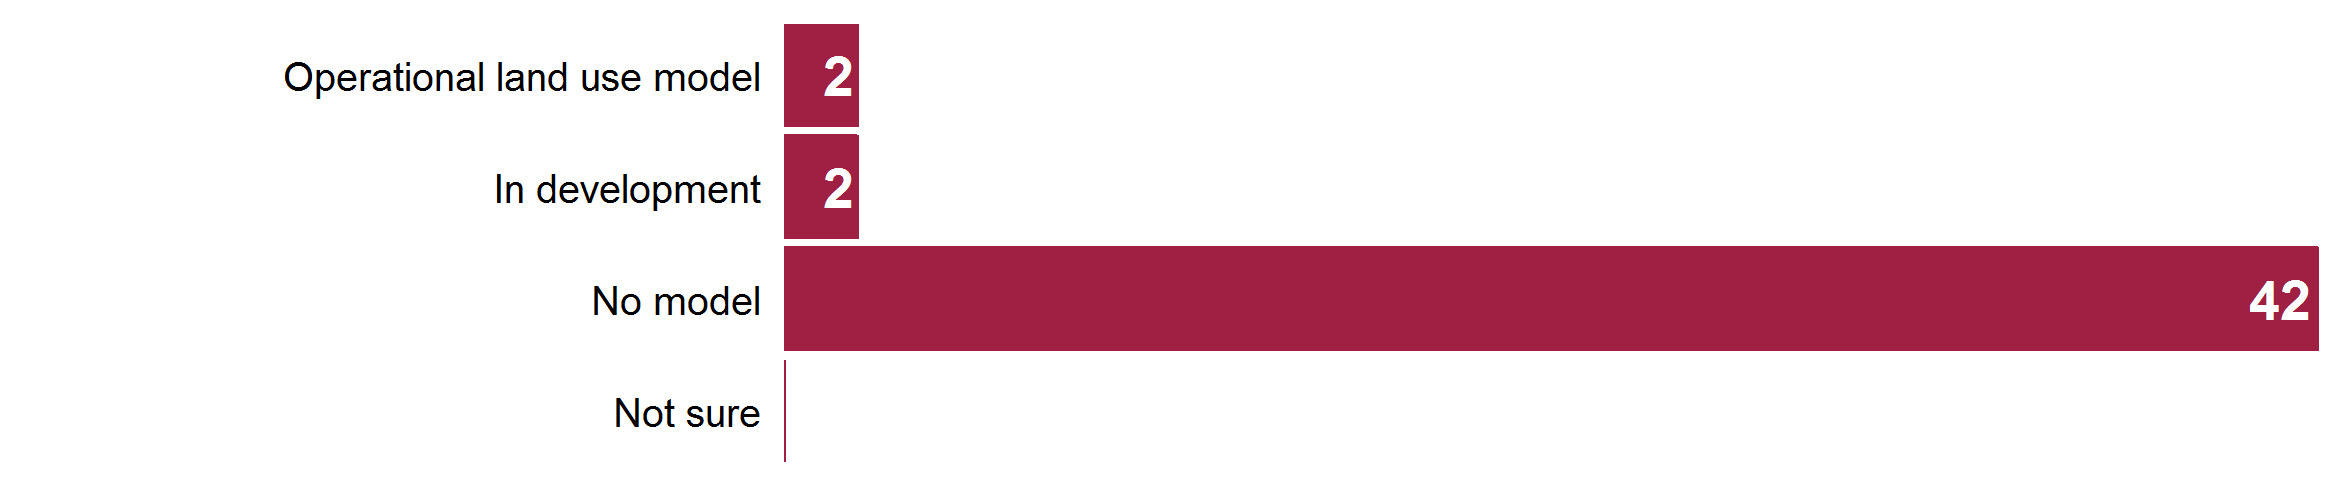
\includegraphics[width=6.4in]{graphics/30-integrated-land-use-transport-models}
\caption{Frequency of integrated land use-transportation models at the statewide level}
\label{fig:integrated-models}
\end{figure}

A clustering of land use models of Oregon/Nevada and Indiana/Ohio can be seen in Figure \ref{fig:land-use-model-states}, which may be entirely coincidental. While at least three more states (California, Florida and Maryland) have operational land use models as well, they have not been integrated with the official version of the statewide transportation model, and therefore do not appear in Figures \ref{fig:integrated-models} and \ref{fig:land-use-model-states}.

\begin{figure}   % 31
\centering
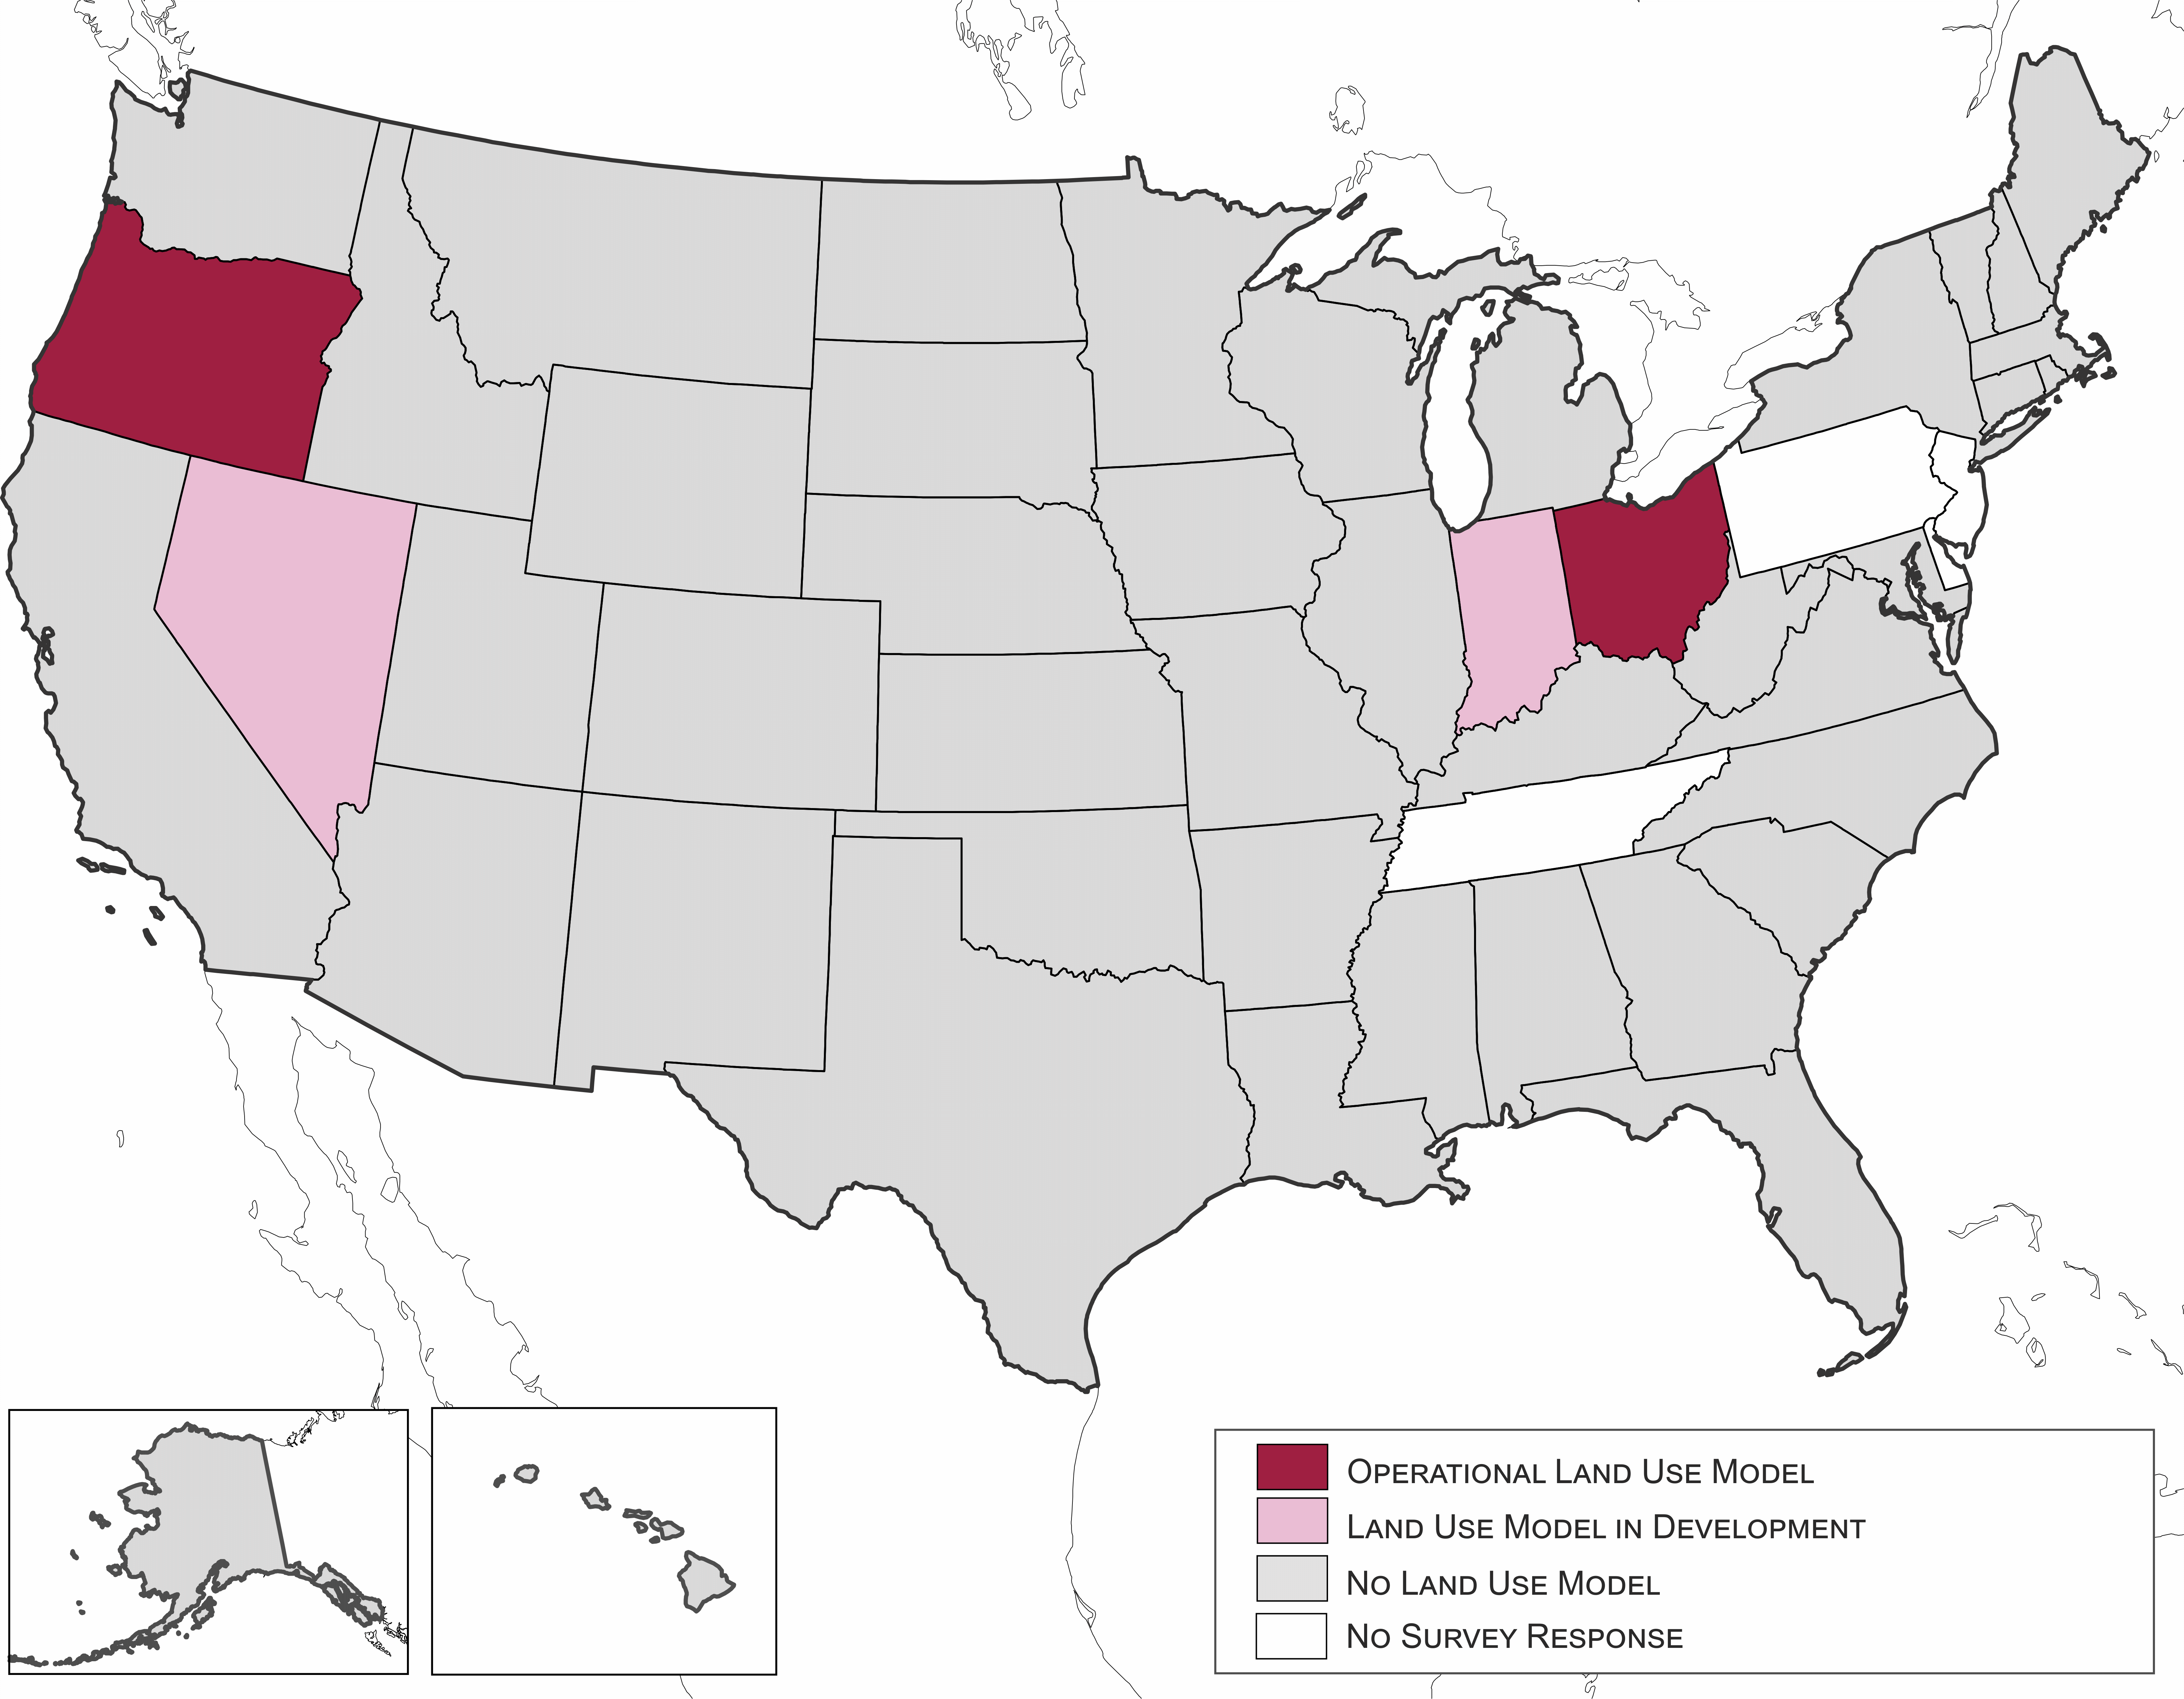
\includegraphics[width=6.5in]{graphics/31-land-use-model-states}
\caption{Distribution of states with land use models}
\label{fig:land-use-model-states}
\end{figure}

\section{Environmental impact models}

Nine states explicitly model the environmental impacts of traffic flows, as shown in Figure \ref{fig:environmental-model-frequency}. This number is relatively small, given that it is common practice to model environmental impacts with urban models. All cases reported referred only to air quality. In research environments, models to analyze the impact on water quality have been developed (see \S\ref{sec:chesapeake-bay-megaregion-model} and \cite{baker07}), though such models have not yet been applied in practice.

\begin{figure}   % 32
\centering

\includegraphics[width=6.4in]{graphics/32-environmental-model-frequency}
\caption{Frequency of environmental impact modeling within statewide models}
\label{fig:environmental-model-frequency}
\end{figure}

The spatial distribution of states with environmental impact models is shown in Figure \ref{fig:environmental-model-states}. It is notable that all West Coast states (of the lower 48 states) model environmental impacts, for environmental issues have traditionally been given more attention than in many other parts of the country. Two Southern states and Michigan also model environmental impacts, and a New England cluster can be seen as well.

\begin{figure}   % 33
\centering
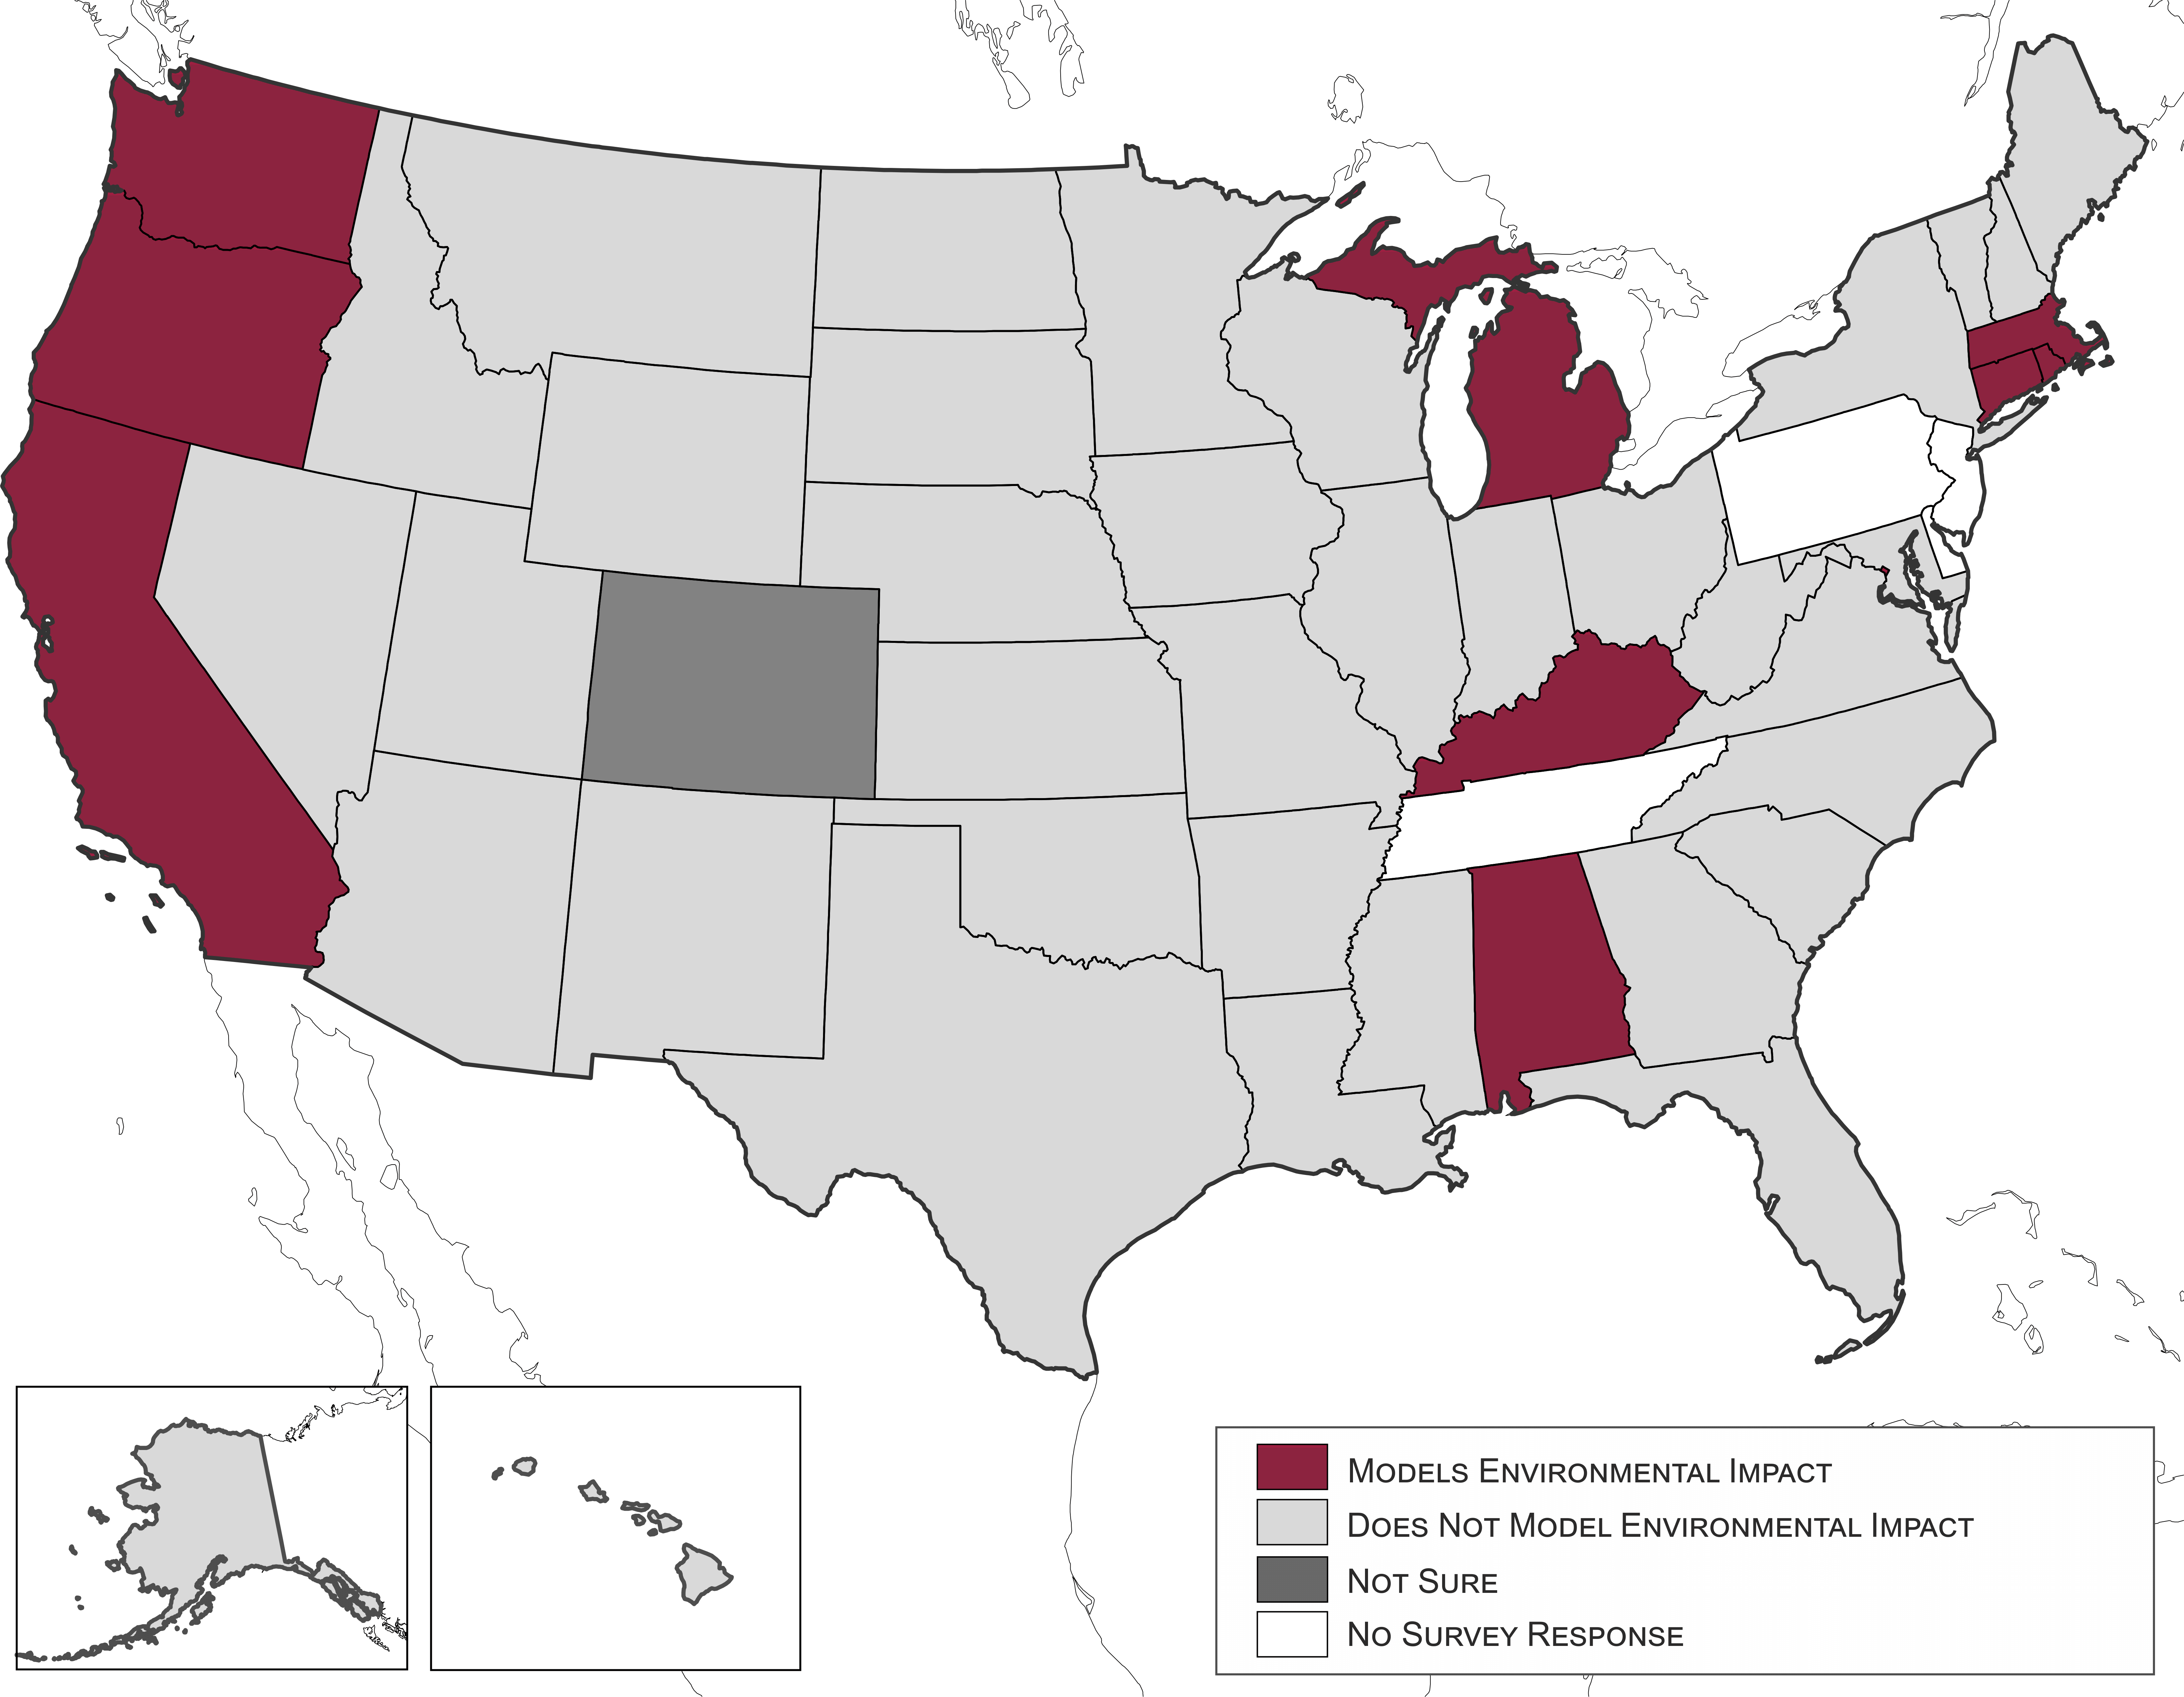
\includegraphics[width=6.5in]{graphics/33-environmental-model-states}
\caption{Distribution of states that model environmental impacts}
\label{fig:environmental-model-states}
\end{figure}

Most states that model environmental impacts use the MOVES model, as shown in Figure \ref{fig:environmental-impact-models}. This model is provided by the Environmental Protection Agency (EPA) at no cost, and is widely accepted as the U.S. standard for modeling air pollutants, greenhouse gases, and air toxics generated by mobile sources. Oregon uses MOVES in combination with their own greenhouse gas model (GreenStep), and Kentucky uses both MOVES and its predecessor, MOBILE. EMFAC is used in California only, based upon emission rates provided by California EPA's Air Resources Board.

\begin{figure}   % 34
\centering

\includegraphics[width=6.4in]{graphics/34-environmental-impact-models}
\caption[Frequency of environmental impacts models]{Frequency of environmental impacts models (multiple answers allowed)}
\label{fig:environmental-impact-models}
\end{figure}

The types of emissions covered are listed in Figure \ref{fig:emissions-modeled}. CO\textsubscript{2}, NO\textsubscript{x} and PM are the most common emissions modeled. Oregon and Washington are the only two states that calculate noise emissions, a significant factor that impacts human health and well-being \citep{decoensel05}. Other analyzed emissions reported included VOC (Connecticut, Kentucky, Massachusetts), CO (Massachusetts) and O\textsubscript{3} (Rhode Island).

\begin{figure}   % 35
\centering
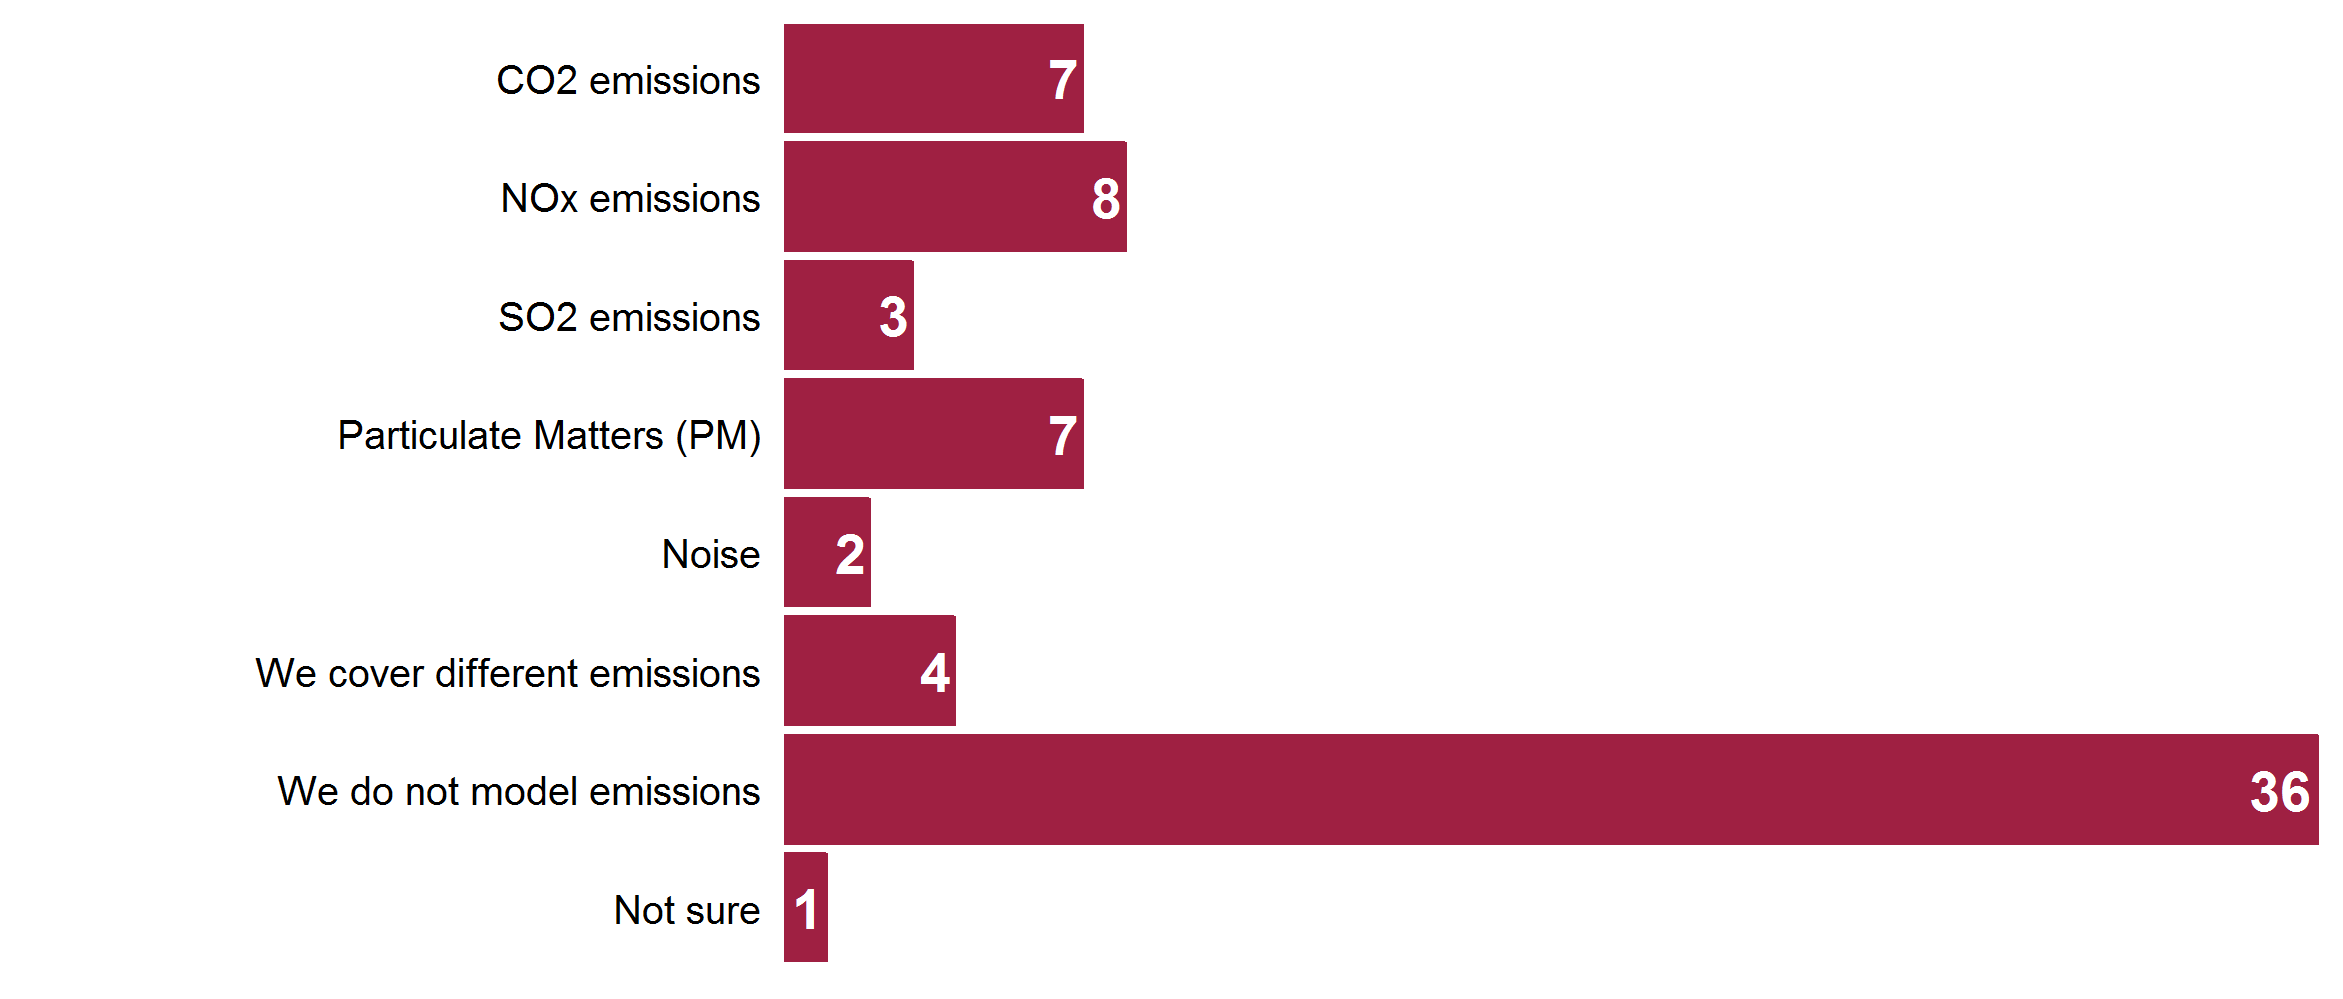
\includegraphics[width=6.4in]{graphics/35-emissions-modeled}
\caption[Emissions modeled with statewide models]{Emissions modeled with statewide models (multiple answers allowed)}
\label{fig:emissions-modeled}
\end{figure}

\section{Resources}

Agencies that operate statewide models were asked about the resources they have invested in model development and application. The first question asked for the number of full-time equivalent employees. Answers ranged from zero to six full-time equivalent employees, with an average of 1.6, as shown in Figure \ref{fig:staffing}. Note that each bar represents a range; for example, the left-most bar stands for five agencies that have between zero and 0.5 full-time equivalent employees.

\begin{figure}   % 36
\centering
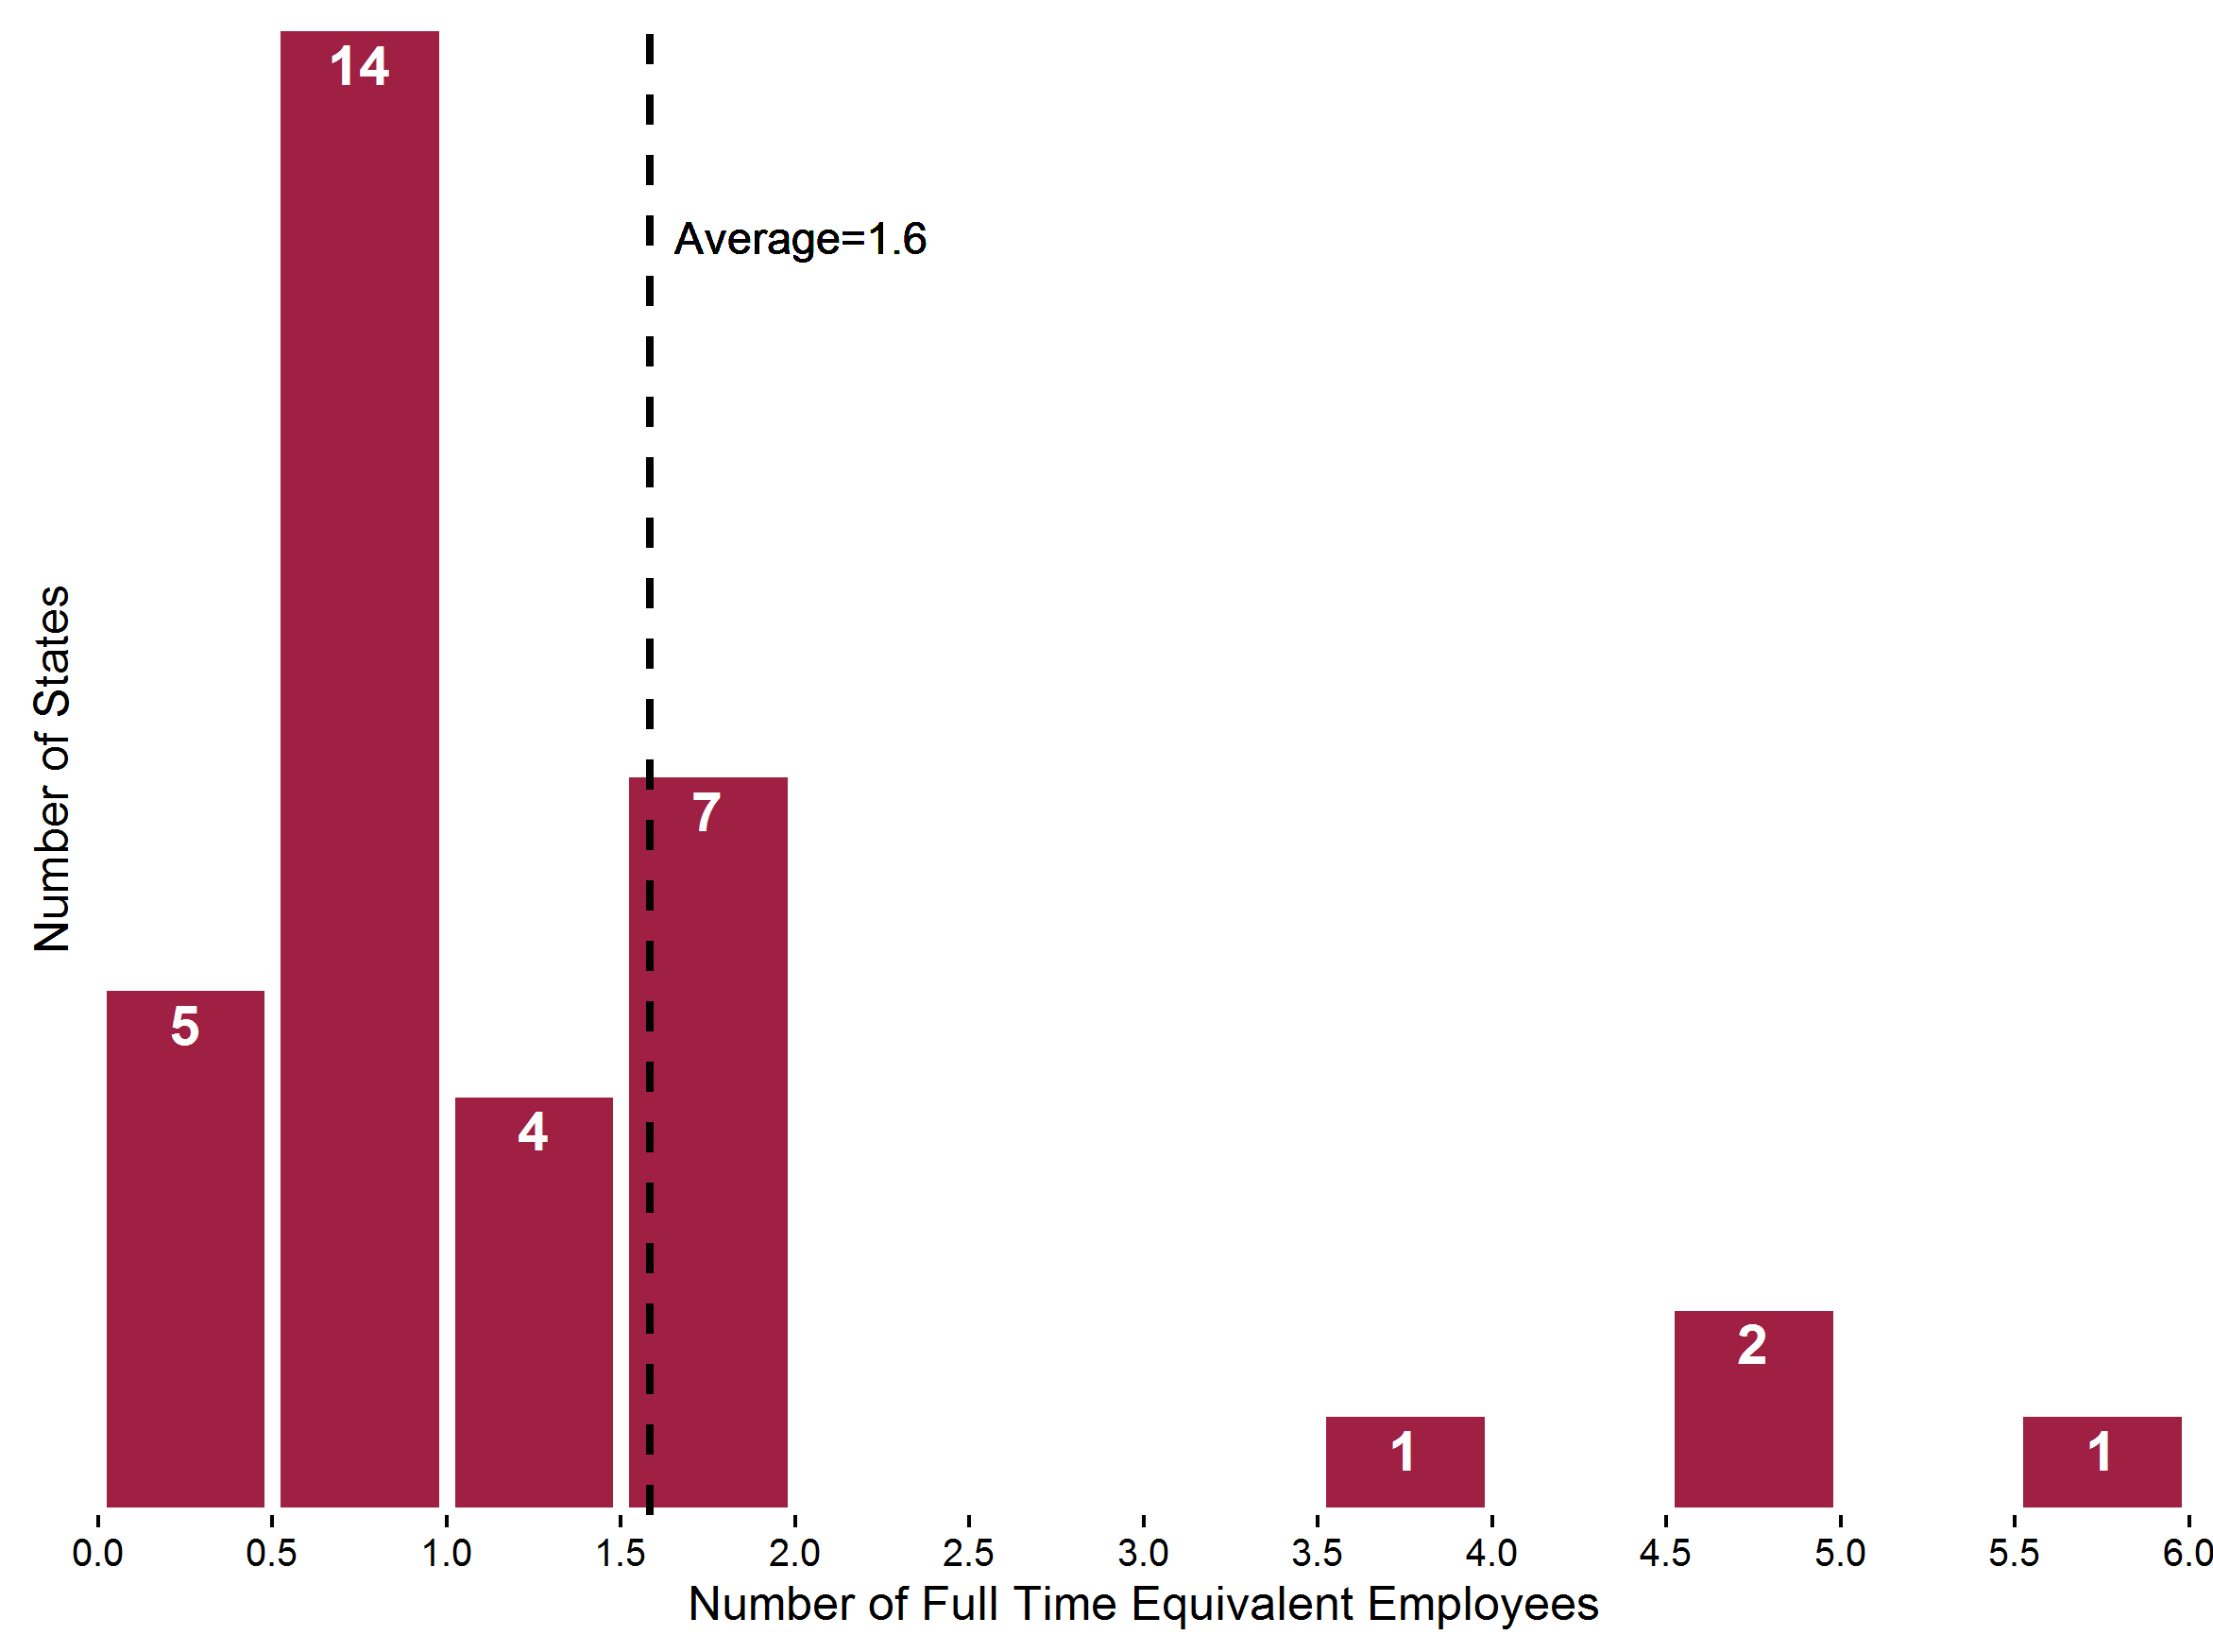
\includegraphics[width=5.8in]{graphics/36-staffing}
\caption{Number of full-time equivalent employees working on statewide modeling}
\label{fig:staffing}
\end{figure}

For model development, a relatively large share of resources (71 percent) were allocated to consultants on average, plus another eight percent being allocated to universities (Figure \ref{fig:resource-allocation}). Only 20 percent of the resources were invested in-house or for partner agencies. On the one hand, this means that a lot of expertise in model development is found outside the state agency. On the other hand, it might be considered neither cost efficient nor practical to train staff to build a model, a task faced by the agency maybe every 10 to 20 years.

\begin{figure}   % 37
\centering
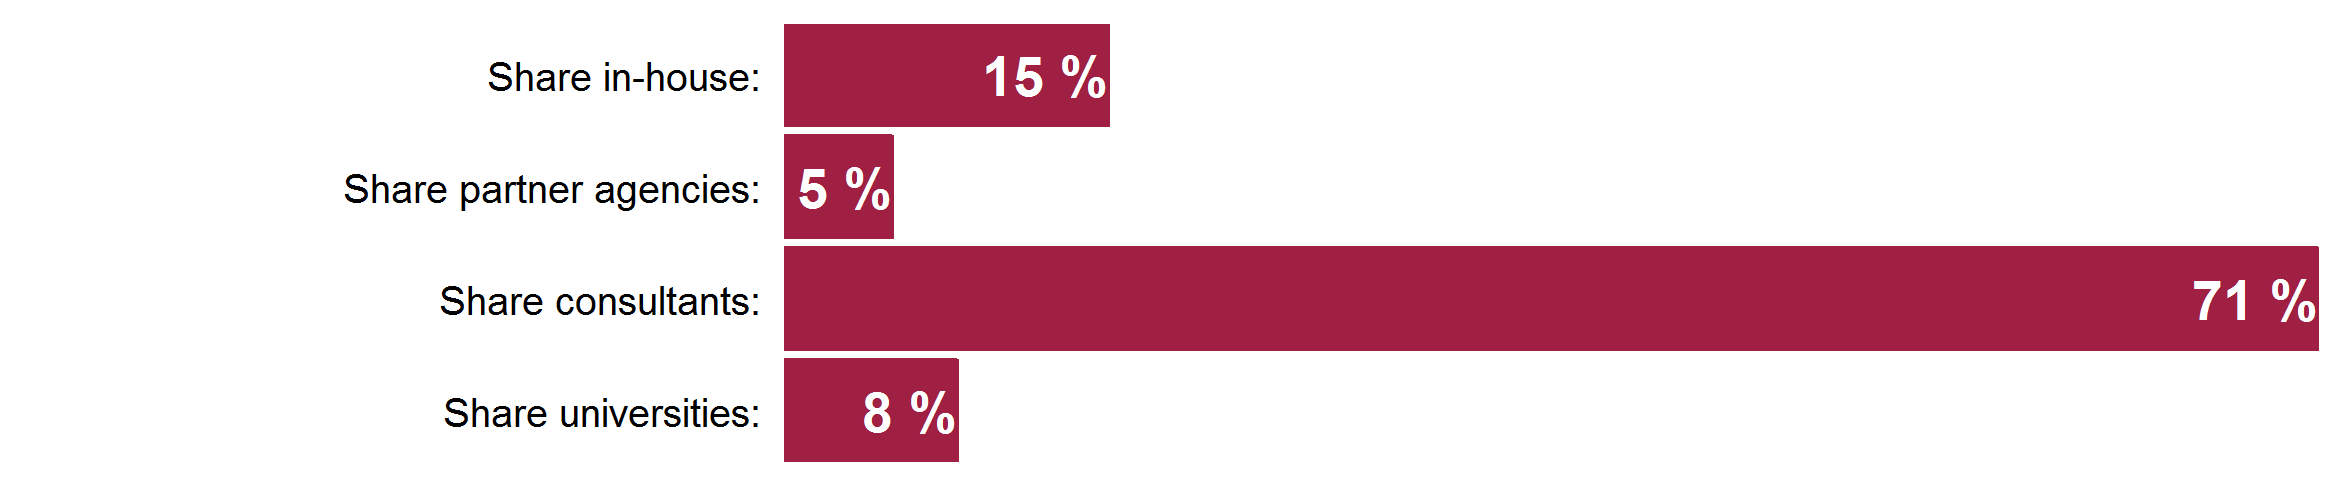
\includegraphics[width=6.4in]{graphics/37-development-resource-allocation}
\caption{Resource allocation for model development}
\label{fig:resource-allocation}
\end{figure}

For model application, the percentages are almost completely reversed, as shown in Figure \ref{fig:application-resource-allocation}. In-house and partner agencies on the average conduct 60 percent of the model application work. Compared to model development, the share for consultants and universities drops in half. While this general trend was expected, the combined 39 percent of outside support for model development is rather large. Except for highly specialized scenarios or short-term staff shortages, state agencies would benefit greatly from avoiding outsourcing of model applications, and instead building this capacity in-house.

\begin{figure}   % 38
\centering
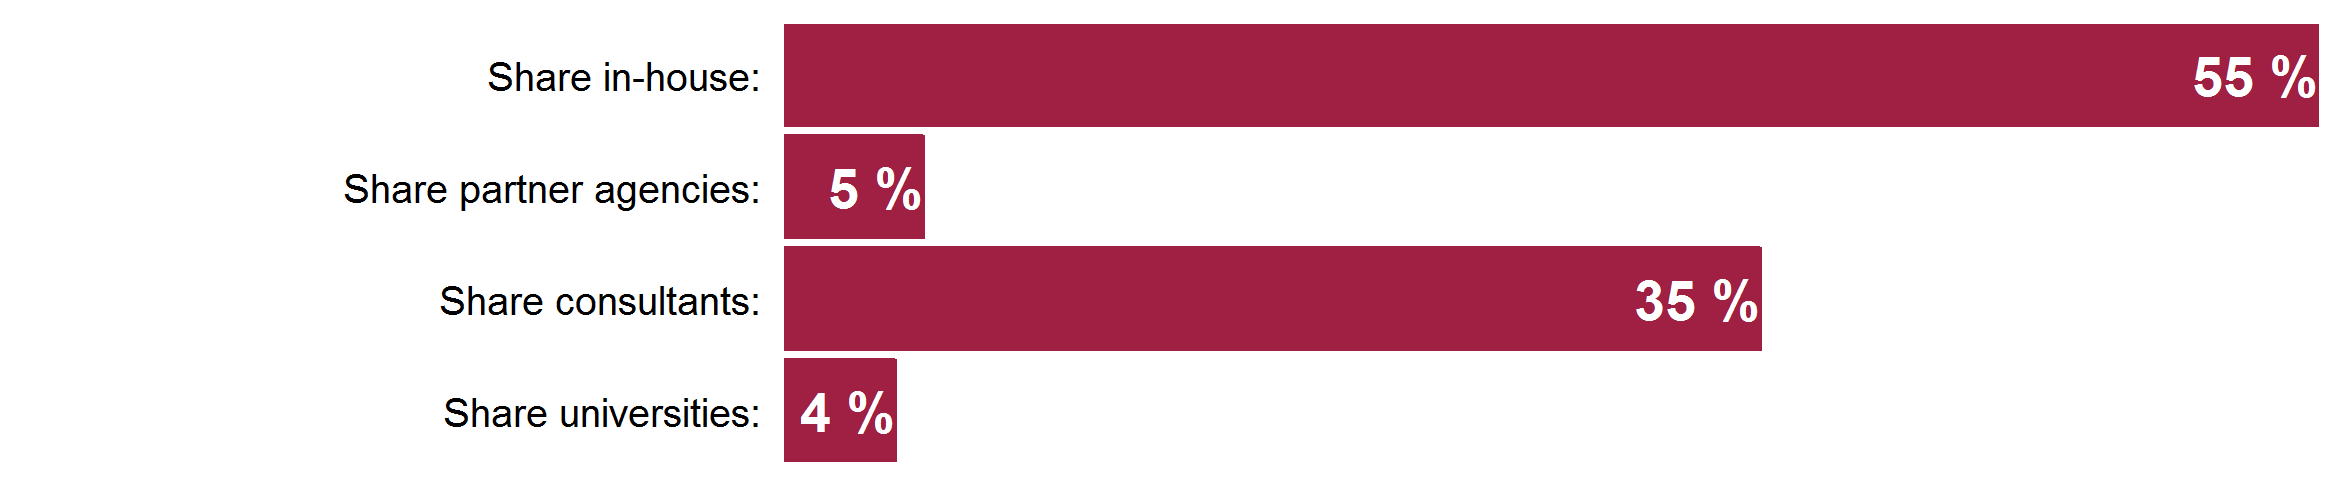
\includegraphics[width=6.4in]{graphics/38-application-resource-allocation}
\caption{Resource allocation for model application}
\label{fig:application-resource-allocation}
\end{figure}

Finally, the questionnaire asked how much money was invested into the model over the past several years. The estimate does not include costs for staff within the agency, but only expenditures for data purposes, software licenses, and outside help. Several states noted that it was difficult to retrieve these numbers, and that they likely had spent more money than reported. In some cases, the most expensive data were collected more than 10 years ago, making numbers for some states seem low.

Given these uncertainties, the expenditures for last year appeared most relevant. On the average, agencies spent \$700,000 on statewide modeling. However, last year's expenditures were highly skewed by one agency that reported spending \$11 million. The standard deviation for this average is \$2 million, almost three times the average. Removing this one outlier reduces last year's average expenditure to \$340,000, which appears to represent the average better. Obviously, agencies developing a model need to invest significantly more for its initial development, while other agencies with mature models will be able to function with substantially less money. Likewise, a new household travel survey would require a substantial expenditure, but such data investments will only be required every couple of years.

The survey replies also indicated that most agencies spend money on their model continuously. Even though agencies with mature models tended to spend less money in recent years, continuous efforts to update input data, revise models to keep up with the state-of-practice and training new staff members required continued investment to sustain an effective statewide model. However, outside of major overhaul efforts, a few hundred thousand dollars seemed to be sufficient for maintaining an operational model, although this might vary depending upon the availability and capabilities of in-house staff.

\section{Critical review of the survey methodology}\label{sec:survey-critical-review}

Best practices of survey research (e.g., \cite{babbie11}) were applied when conducting the survey on statewide modeling among all U.S. states. The questionnaire was developed and revised based on comments from the review panel overseeing this synthesis report. The online survey tool was reviewed and refined by four different scientists. A pretest was conducted that helped fine-tune contents. Sensitive questions (on staffing and budget) were asked towards the end. The survey request was sent out by TRB with an email explaining the relevance of the study. Contact information for questions was provided, and late respondents were reminded several times by email and telephone. Nevertheless, survey results need to be interpreted with some caution.

It turned out that some survey responses were inconsistent. They were reviewed carefully, and corrected if it was obvious what was intended. This happened repeatedly on the budget question, for example. A few states responded that they spent money in the last year, but then left the field for expenditures over the last two years empty. In that case, the amount spent in the last year was assumed to apply to the last two years as well. In other cases, the intended answer was not as obvious. For example, a few states reported that they do not model environmental impacts, yet did report modeled types of environmental emissions. It could not be determined from the responses whether those states conducted environmental modeling or not. 

In at least one case it was found that emission estimates from the traffic assignment model were compiled in a manual post-processor rather than using a separate emissions model. Several phone calls and follow-up emails were necessary to disentangle inconsistencies. In one case, two respondents from the same state filled out a survey but provided different answers to some questions. These inconsistencies were corrected by contacting both respondents to seek clarifications. In a few cases, however, clarification could not be obtained by contacting the respondent, for sometimes they were unsure about model design details.

Future studies should consider setting aside sufficient time and resources to conduct phone interviews instead of online surveys with every state to avoid such inconsistencies. Such interviews would not be trivial to complete, as in several cases respondents would have to research answers before the interview could be completed later. A considerably higher effort of contacting, scheduling, and conducting the interviews would be required. While such an approach would require a substantially higher effort, it appears to be the only viable approach to collect detailed information on complex systems without inconsistencies in the answers.

\section{Summary findings of the survey}

Despite some shortcomings, the survey provided intriguing findings on statewide modeling in the U.S. It is remarkable how statewide modeling has become a standard practice in most states. Given the complexity of the transportation system and the intricacy of policy questions posed by decision makers today, transportation planning agencies cannot continue to rely on intuition and experience alone. Most states make heavy use of statewide models, some of them quite sophisticated, to support decision making in transportation planning.

At the same time, it became obvious that urban models tend to be more advanced than statewide models. When comparing the 34 operational statewide models with the 34 largest urban models, the latter show substantially more complexity and rigor \citep{donnelly10}. For example, only five statewide models reported using a tour-based approach, while more than a dozen urban models do so. There are five statewide models still using multiple regression for trip generation, a concept that has mostly disappeared from urban models. While urban models without mode choice models have become rare, six statewide models use static mode shares, and another 12 ignore different modes of transport entirely. Most remarkable is the fact that 20 out of 34 models do not distinguish time of day, but rather generate daily traffic. Reasonable estimations of congestion are near impossible without distinguishing between peak and off-peak travel conditions.

An attempt to compare the distribution in terms of the level of development found in statewide models with urban models is shown in Figure \ref{fig:model-development-comparison}. While both very simple and highly sophisticated model designs can be found in both statewide and urban models, the average urban models appear to be further developed than the average statewide model.

\begin{figure}   % 39
\centering
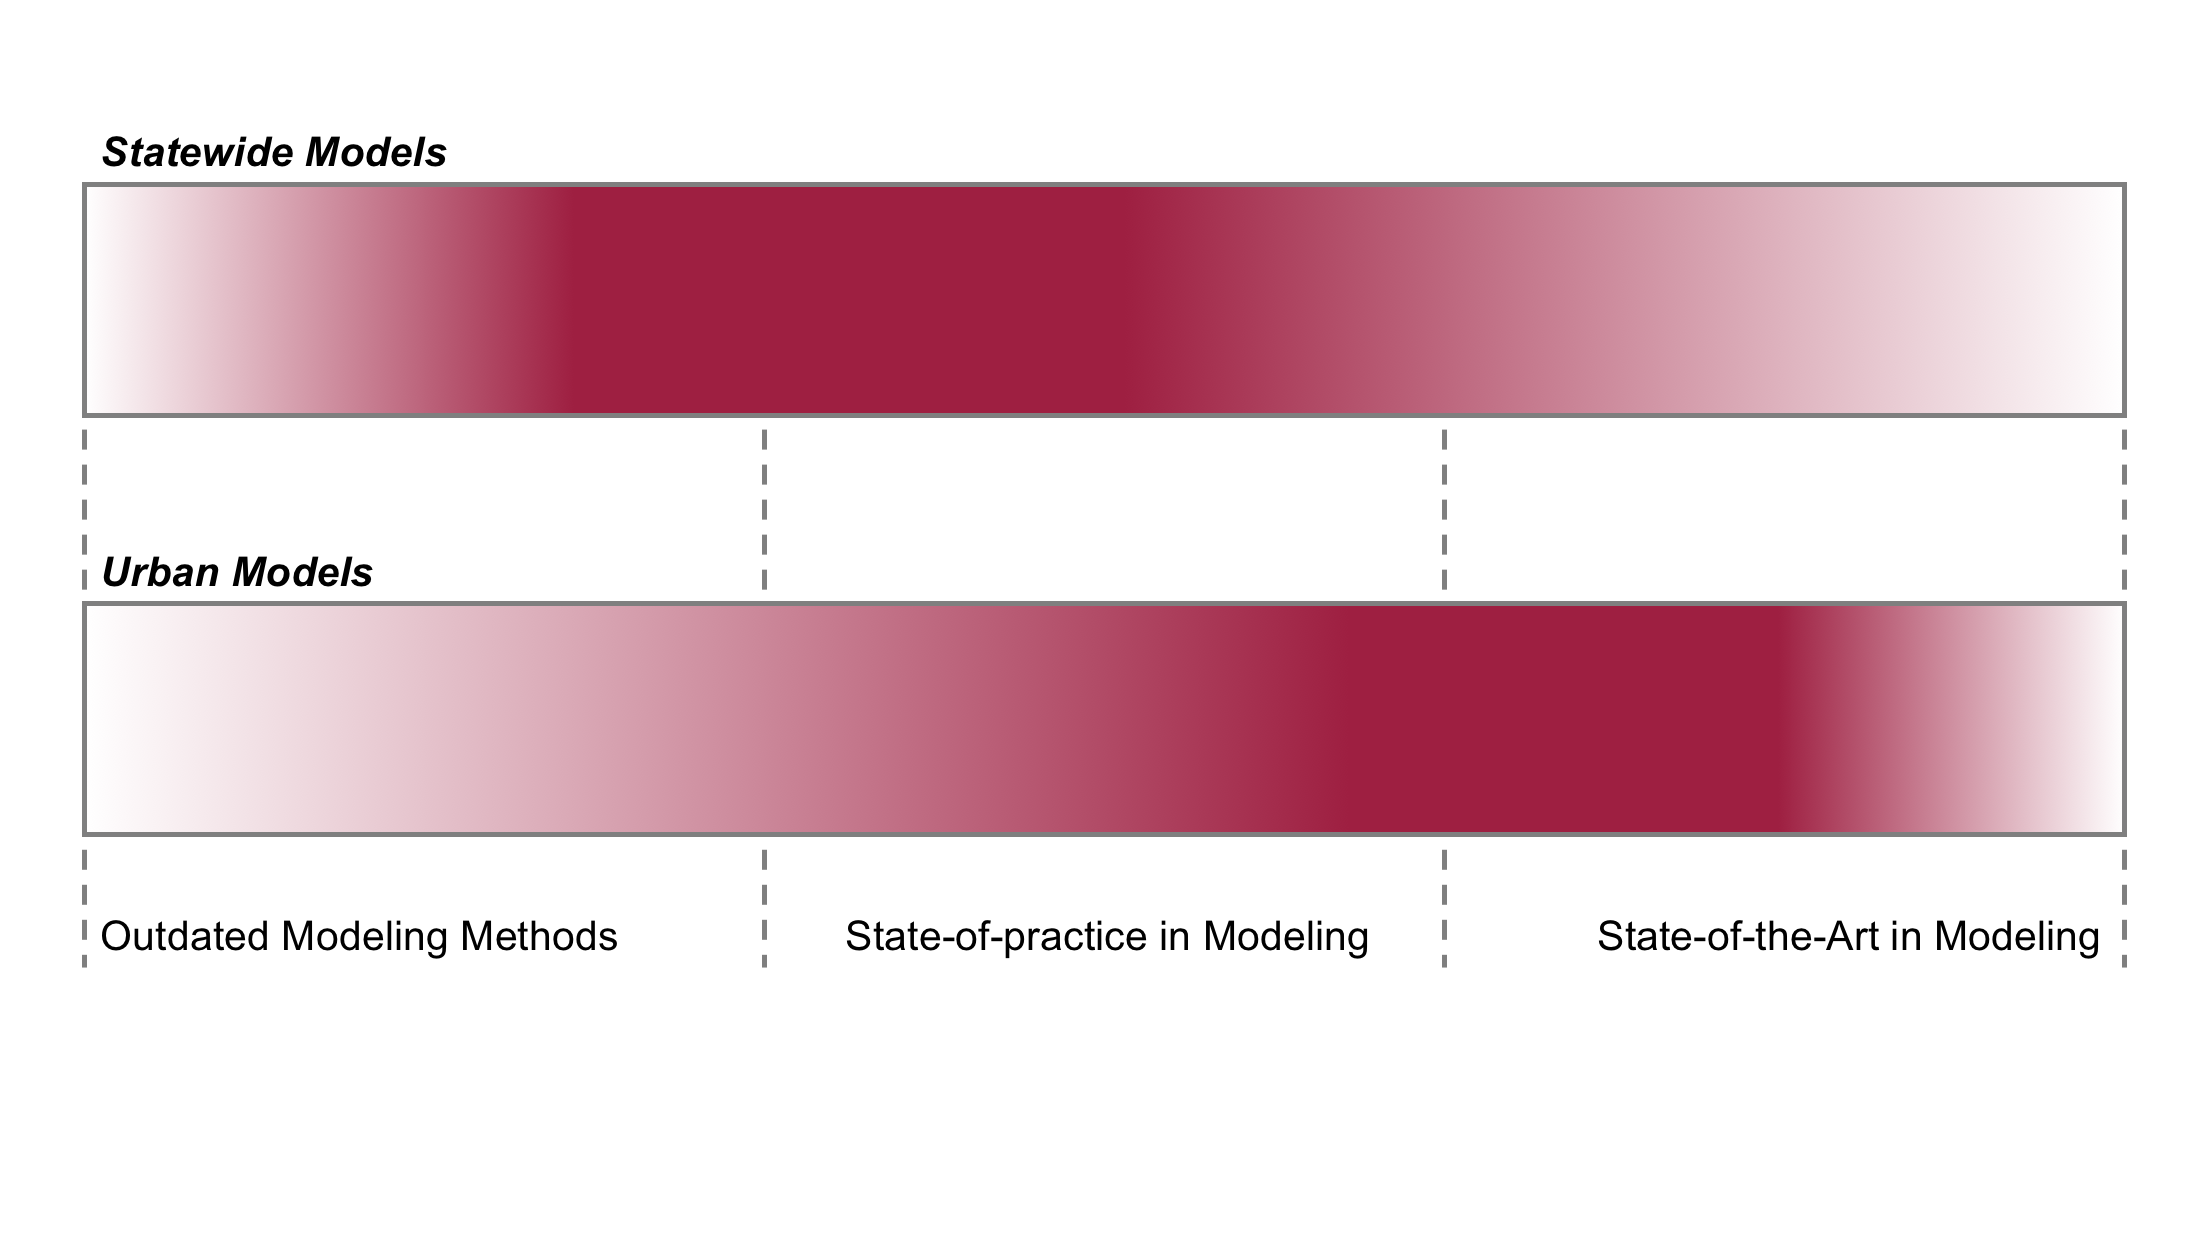
\includegraphics[width=6.4in]{graphics/39-model-development-comparison}
\caption{Attempt to compare level of development of statewide models with urban models}
\label{fig:model-development-comparison}
\end{figure}

However, the fact that statewide models tend to be simpler is not a critique per se. Simpler models may well can answer questions asked in each state. If two models could answer the questions at hand, the simpler model should always be preferred as it limits the risk of model inconsistencies. As Albert Einstein is said to have noted, ``a model should be as simple as possible, yet no simpler.'' Moreover, the temporal, spatial, and behavioral resolutions found in many state-of-the-art urban models would be prohibitively costly if extended to cover an entire state. It appears that most model developers have attempted to balance the desire for greater capabilities with pragmatic concerns about computational and data burdens associated with such models.

Efforts to integrate several statewide models with analytics from other related domains are particularly worthy of praise. Fifteen states operate separate models for person long-distance travel; truck travel is represented explicitly in 21 models for short-distance travel and in 26 models for long-distance freight flows. Another 11 states include some form of a freight mode choice model, an inherently complex undertaking. Finally, six states operate their own economic forecasting model, and two have an operational land use model. Statewide models tend to be more advanced than the average urban model in terms of these interdisciplinary modeling approaches.